\documentclass[11pt]{article}
\ifdefined\pdfinfoomitdate\pdfinfoomitdate=1\fi
\ifdefined\pdftrailerid\pdftrailerid{}\fi
\ifdefined\pdfsuppressptexinfo\pdfsuppressptexinfo=15\fi
\usepackage[T1]{fontenc}
\usepackage[utf8]{inputenc}
\usepackage{lmodern}
\usepackage[margin=1in]{geometry}
\usepackage{amsmath,amssymb,amsthm,mathtools}
\usepackage{microtype}
\usepackage{enumitem,booktabs,array}
\usepackage{tikz}
\usepackage{placeins,flafter}
\usepackage[titles]{tocloft}
\usepackage[hyphens]{url}
\usetikzlibrary{arrows.meta,positioning,calc}
\usepackage{xcolor}
\definecolor{linkblue}{RGB}{25,63,105}
\usepackage[colorlinks=true,allcolors=linkblue,pdfencoding=auto,psdextra]{hyperref}
\usepackage[nameinlink,capitalise,noabbrev]{cleveref}
\hypersetup{
  pdftitle={The Unique Games Theorem},
  pdfsubject={A deterministic reduction from 3SAT to Unique Games},
  pdfauthor={OpenAI},
  pdfkeywords={Unique Games, approximation hardness, shortcode, projection games}
}

\newtheorem{theorem}{Theorem}[section]
\newtheorem{lemma}[theorem]{Lemma}
\newtheorem{proposition}[theorem]{Proposition}
\newtheorem{corollary}[theorem]{Corollary}
\theoremstyle{definition}
\newtheorem{definition}[theorem]{Definition}
\theoremstyle{remark}
\newtheorem{remark}[theorem]{Remark}
\numberwithin{equation}{section}
\newcommand{\F}{\mathbb F}
\newcommand{\E}{\mathbb E}
\newcommand{\eps}{\varepsilon}
\DeclareMathOperator{\OPT}{OPT}
\DeclareMathOperator{\val}{val}
\DeclareMathOperator{\Hom}{Hom}
\DeclareMathOperator{\im}{im}
\DeclareMathOperator{\rank}{rank}
\DeclareMathOperator{\Span}{span}
\DeclareMathOperator{\supp}{supp}
\DeclareMathOperator{\TV}{TV}
\newcommand{\abs}[1]{\lvert #1\rvert}
\newcommand{\norm}[1]{\lVert #1\rVert}
\newcommand{\ip}[2]{\langle #1,#2\rangle}
\setlist[itemize]{topsep=4pt,itemsep=2pt,parsep=0pt}
\setlist[enumerate]{topsep=4pt,itemsep=2pt,parsep=0pt}
\setlength{\emergencystretch}{2em}
\allowdisplaybreaks[1]

\title{The Unique Games Theorem}
\author{OpenAI}
\date{September 23, 2026}

\begin{document}
\maketitle
\begin{abstract}
We prove the Unique Games Conjecture. For every fixed
\(\varepsilon,\delta\in(0,1/2)\), we give a deterministic polynomial-time
reduction from \(\mathrm{3SAT}\) to Unique Games over a fixed finite alphabet,
with completeness at least \(1-\varepsilon\) and soundness at most \(\delta\).
\end{abstract}

\begingroup
\small
\setlength{\baselineskip}{10.5pt}
\setlength{\cftbeforesecskip}{3pt}
\tableofcontents
\endgroup
\clearpage
\section{Introduction}\label{sec:introduction}

A permutation constraint prescribes exactly one label at one endpoint for
each label at the other. The Unique Games Conjecture asserts that systems
of such constraints can be hard to approximate even when almost all
constraints can be satisfied. We resolve this conjecture positively, with an
explicit unweighted reduction from \(\mathrm{3SAT}\).

\subsection{The theorem}

A \emph{Unique Games instance} has a finite vertex set, a finite alphabet
\(K\), and a nonempty list of oriented constraints
\(e=(u_e,v_e,\pi_e)\), where \(\pi_e\) is a permutation of \(K\).
A labeling \(a\) satisfies \(e\) when
\(a(v_e)=\pi_e(a(u_e))\). Its value is the fraction of satisfied
constraints, and \(\val(G)\) is the maximum value of a labeling.
The instance is \emph{explicit and unweighted} when the entire vertex
and constraint lists are written out, including the table of each
permutation. A simple bipartite instance has two disjoint vertex sets
and at most one constraint on each pair of opposite vertices.

\begin{theorem}[Unique Games Theorem]\label{thm:ugc}
For every fixed \(\varepsilon,\delta\in(0,1/2)\), there are an integer
\(s\ge1\) and a deterministic polynomial-time reduction from
\(\mathrm{3SAT}\) to explicit unweighted Unique Games instances
\(G_\varphi\) over \(K=\F_2^s\) such that
\[
\begin{aligned}
 \varphi\text{ satisfiable}
 &\quad\Longrightarrow\quad \val(G_\varphi)\ge1-\varepsilon,\\
 \varphi\text{ unsatisfiable}
 &\quad\Longrightarrow\quad \val(G_\varphi)\le\delta.
\end{aligned}
\]
The graph is simple and bipartite, and every constraint is a translation
\(a(v_e)=a(u_e)+c_e\) of \(K\). The alphabet, the degree of the
running-time polynomial, and its constants depend only on
\(\varepsilon,\delta\).
\end{theorem}

Thus the result resolves the Unique Games Conjecture positively in its
usual edge-value formulation~\cite[Conjecture~2.5]{Khot10}.
The two errors are prescribed independently, before the alphabet is chosen.
Binary translation constraints are a known equivalent formulation of the
conjecture~\cite[Corollary~13 and Section~11.1]{KKMO07}; the reduction
here produces that form directly.

Theorem~\ref{thm:ugc} supplies the Unique Games hypothesis in earlier
hardness reductions for cut, covering, constraint-satisfaction, ordering,
deletion, and clustering problems
\cite{KKMO07,KhotRegev2008,Raghavendra08,GuruswamiEtAl2011OrderingCSP,CKKRS2006,DemaineEtAl2006Clustering}.
The reductions and the resulting approximation thresholds are due to
those authors. Section~\ref{sec:consequences} gives the precise problem
formulations, strict thresholds, and reduction qualifications, together
with proofs of the consequences.

\subsection{Proofs, codes, and the quantifiers}

The central difficulty is to retain completeness near one when every
label permits only one reply. The earlier connection between proof
verification and approximation hardness was developed by Feige,
Goldwasser, Lov\'asz, Safra, and Szegedy~\cite{FGLSS96}, by Arora and
Safra through proof composition~\cite{AroraSafra98}, and by Arora,
Lund, Motwani, Sudan, and Szegedy through the constant-query PCP
theorem~\cite{ALMSS98}. Bellare, Goldreich, and Sudan introduced the
long code and folding for verifier composition~\cite[Section~3.3]{BGS98}.
The long code of an answer \(a\) is the table \(f\mapsto f(a)\),
indexed by Boolean functions on the answer set. In H\aa stad's
parity-hardness proof, Fourier analysis recovers an outer-game strategy
from arbitrary proof tables that make his verifier accept sufficiently
often, without first recovering nearby codewords. His nearly satisfiable
parity gap is our starting hardness input~\cite{Hastad01}.

Khot introduced the Unique Games Conjecture in 2002 and gave an algorithm
based on semidefinite rounding~\cite{Khot02}.
Several algorithmic guarantees explain why its order of quantifiers
matters. For a fixed target error, Trevisan combines semidefinite rounding
with graph decomposition to obtain a polynomial-time
guarantee when the input error shrinks at the reciprocal-logarithmic
rate in the instance size~\cite{Trevisan08}. Charikar, Makarychev, and
Makarychev use randomized semidefinite rounding to obtain expected value
\(1-O(\sqrt{\epsilon\log q})\) from
a \(q\)-label instance of value at least \(1-\epsilon\)~\cite{CMM06};
this guarantee loses accuracy as the alphabet grows, whereas the
conjecture permits a large fixed alphabet after the errors are chosen.
Kolla's spectral enumeration gives a running-time bound in terms of the
dimension of a suitable spectral subspace of the label-extended graph,
whose vertices are variable--label pairs~\cite{Kolla11}. Arora, Barak, and Steurer use
spectral decomposition and enumeration to obtain near-satisfying
solutions for sufficiently small fixed completeness error, with a
guarantee independent of the fixed alphabet size~\cite{ABS10}; their
running-time bound is subexponential, not polynomial, for fixed positive
error. These are distinct limits on the known guarantees.

Integrality gaps concern the strength of a relaxation. Khot and Vishnoi
constructed Unique Games with semidefinite value arbitrarily close to
one and integral value arbitrarily close to zero, even with triangle
inequalities~\cite{KV15}. Barak, Gopalan, H\aa stad, Meka, Raghavendra,
and Steurer introduced the short code, based on Reed--Muller codes, as a
shorter substitute for the long code in applications including alphabet
reduction and quantitative integrality gaps~\cite{BGHMRS15}. These constructions constrain particular
relaxations; a hardness reduction requires a separate argument.
Bafna, Barak, Kothari, Schramm, and Steurer obtain polynomial-time
constant-value guarantees for nearly satisfiable translation games
whose graphs have suitable low-degree sum-of-squares hypercontractivity
certificates, including noisy hypercube and noisy Reed--Muller short-code
graphs~\cite{BBKSS21}. The rank-one matrix shortcode used below is a
different graph, and our argument does not assume these certificates.

\subsection{Grassmann expansion and the completeness obstacle}

The closest preceding hardness breakthrough concerns 2-to-1 and
2-to-2 games with imperfect completeness. A 2-to-1 constraint is a
projection with exactly two preimages per right label. A 2-to-2
constraint partitions the labels on each side into pairs and matches
these pairs bijectively, allowing the four combinations within a
matched pair. Khot, Minzer, and Safra's STOC~2017 work proposed a
Grassmann-graph reduction whose nonstandard soundness guarantee was
conditional on a structural hypothesis~\cite{KMS17}. Dinur, Khot,
Kindler, Minzer, and Safra's STOC~2018 work proposed a reduction with
ordinary edge-satisfaction soundness, conditional on an agreement
hypothesis~\cite{DKKMS25}; their expansion work formulated the relevant
structural problem and established partial cases~\cite{DKKMS21Expansion}.
Barak, Kothari, and Steurer connected expansion to the needed agreement
test through a binary matrix representation~\cite{BKS18}. The expansion
theorem of Khot, Minzer, and Safra completed this line in
2018~\cite{KMS23}.

These results established hardness for almost satisfiable 2-to-1 and
2-to-2 games and, as a consequence, a Unique Games gap with completeness
close to one half and arbitrarily small soundness. Obtaining Unique
Games completeness arbitrarily close to one was a separate problem.\footnote{A
separate companion proves hardness for exact 2-to-1 games with perfect
completeness and arbitrarily small fixed soundness, over fixed
alphabets~\cite[Theorem~1.1]{OpenAIPerfectTwoToOne2026}. It is not an input
to this proof.}

The degree-two matrix shortcode of Barak, Kothari, and
Steurer~\cite{BKS18} is the formulation used here: its vertices are
binary matrices and its steps add rank-one matrices. Their two-reply rule
permits either the old answer or its translate by the update's left factor;
requiring equality alone gives a one-half completeness guarantee. They
discussed higher-degree tests as a possible route to improving this
completeness~\cite[Section~1.6]{BKS18}. The inverse statement we use,
derived from Grassmann expansion, appears in Theorem~\ref{thm:shortcode}.
Ellis, Kindler, and Lifshitz later gave a shorter expansion proof using
hypercontractivity on spaces of linear maps~\cite{EKL26}; our external
input remains the Khot--Minzer--Safra theorem. Our proof keeps the
established degree-two inverse theorem and changes the noise using a
nonlinear map. The following comparison explains that choice.

\subsection{The construction and proof}

The uniform rank-one test illustrates the completeness problem. Let
\(M\) be a binary \(\ell\)-by-\(m\) matrix and fix a nonzero answer
\(z\in\F_2^m\). The evaluation function \(f_z(M)=Mz\) satisfies
\[
 f_z(M+a l^\top)-f_z(M)=a(l^\top z).
\]
For independent uniform \(a\in\F_2^\ell\) and \(l\in\F_2^m\), this
evaluation keeps its value with probability \((1+2^{-\ell})/2\), close
to one half. Our test changes the noise while retaining the ordinary
rank-one test as the structural tool for soundness.

For any prescribed \(p>0\), Lemma~\ref{lem:latent} fixes a rank threshold
and, for every sufficiently large \(\ell\), constructs a binary space
\(\mathcal V\) containing \(K=\F_2^\ell\), a map
\(C:\mathcal V\to K\), and a noise law \(\mu\) on \(\mathcal V\)
such that, for \(a\sim\mu\),
\[
 C(x+h)=C(x)+h\quad(h\in K),\qquad
 \Pr[C(x+a)\ne C(x)]\le p
\]
where \(x\) is uniform and independent of \(a\). At the same time, every
family of linear observations
whose restrictions to \(K\) have sufficiently large rank detects
\(a\) with probability at least \(1/8\). The rank threshold depends
only on \(p\) and is chosen before \(\ell\). The construction uses
quadratic blocks over a finite field: their nonlinear outputs become
increasingly stable under recursion, while a rank potential controls the
loss of linear observations. Section~\ref{sec:latent} proves this
separation and realizes the output translations as the subspace \(K\).

For the same nonzero \(z\), let \(P\in\Hom(\F_2^m,\mathcal V)\) be
uniform. The nonlinear evaluation \(P\mapsto C(Pz)\) compares the values
\[
 C(Pz)\quad\text{and}\quad C\bigl(Pz+a(l^\top z)\bigr)
\]
under the update \(P\mapsto P+a l^\top\). Here \(Pz\) is uniform in
\(\mathcal V\), independently of the latent noise \(a\), and
\(l^\top z\) is an independent fair bit. Its equality test therefore
fails with probability at most \(p/2\).

We start the reduction from binary parity equations on three distinct
variables. Each equation has four satisfying triples. A table on an equation
tuple \(U=(e_1,\ldots,e_k)\) is an affine map from the product of their
solution planes to \(\mathcal V\), represented by a matrix with
\(m=1+2k\) columns: one intercept column and two slope columns per
equation. Whenever one equation block affects a table only through one
actual bit, its reduced key records that variable and the entire induced
affine map. A projected table and its pullback receive the same key.
Grouping constant \(K\)-translates of keys into a vertex then folds the
answers: a label at the representative determines every translated
answer, and a shared key gives the same restored answer on both domains.
The resulting Unique Games test checks equality of the restored answers
on a table and its rank-one perturbation using the latent noise. A
near-satisfying global parity assignment gives the ideal evaluation above
on every tuple it satisfies, supplying near completeness. The key sharing
adapts Khot and Safra's virtual tables~\cite[Section~1.1]{KS13}, while the
translation orbits adapt the folding principle of Bellare, Goldreich,
and Sudan~\cite[Section~3.3]{BGS98}.

For soundness, suppose a labeling passes this test with probability at
least \(0.99\). A matrix frequency is a tuple
\(g=(g_i)_{i=0}^{m-1}\in(\mathcal V^*)^m\), one functional per column,
with character \((-1)^{\sum_i g_i(P\mathbf e_i)}\), where the
\(\mathbf e_i\) are the standard basis vectors of \(\F_2^m\). Averaging the phase increment of a
rank-one update over the uniform selector \(l\) gives
\[
\begin{aligned}
 \E_{a\sim\mu,l}(-1)^{\sum_i l_i g_i(a)}
   &=\Pr_{a\sim\mu}[g_i(a)=0\text{ for every }i],\\
 \E_{a\text{ uniform in }K,l}(-1)^{\sum_i l_i g_i(a)}
   &=2^{-\dim\Span\{g_i|_K\}}.
\end{aligned}
\]
The first multiplier is nonnegative and, by latent detection, is at most
\(7/8\) when the restriction rank is large. High acceptance therefore
forces a fixed amount of low-rank Fourier mass; the second multiplier
turns this into positive acceptance under the ordinary uniform rank-one
perturbation in \(K\). Using a linear complement
\(\mathcal V=K\oplus W\) fixed with the latent data, write the table as
\(P=(M,T)\), where \(M\) and \(T\) are its \(K\)- and \(W\)-valued
affine components, represented by matrices that include their constant
columns. The ordinary perturbation changes \(M\) and
fixes \(T\). Thus, for a positive fraction of pairs \((U,T)\), the
restored answer as a function of \(M\) often keeps its value under the
ordinary test. For the remaining soundness argument, take \(k\) to be a
sufficiently large integer cube, with the latent and shortcode parameters
fixed. On each such pair, the inverse shortcode theorem supplies
agreement with a target \(Mz+u\), for some \(z\in\F_2^m\) and \(u\in K\),
on a slice defined by at most a fixed number \(r_{\rm s}\) of row equations
and at most \(r_{\rm s}\) column equations.

For an independent uniform linear map \(A:K\to\F_2^{r_{\rm s}}\), the
visible advice about \((M,T)\) is \((A,T,AM)\). Together with \(U\), it
specifies \(T\) and the row fiber \(\{M':AM'=AM\}\) of \(K\)-valued affine
maps on the answer space of \(U\), including their constant terms. An erasure argument
proves that a fixed positive fraction of such data under unrestricted
table sampling on \(U\) admit additional column equations and a target
\(Mz+u\) certifying agreement on a nonempty slice. For each such datum
\((U,A,T,AM)\),
choose one certificate by a fixed rule depending only on that visible datum
and the fixed labeling. Folding then makes the certificate determine a short
nonempty set of valid answers on \(U\).

The advice experiment compares the equation tuple \(U\) with a question
\(O\) that independently replaces each equation by one uniformly chosen
variable with probability \(\beta\). Let \(\pi\) be the resulting
projection of actual answers. The referee samples a uniform table
\((M_O,T_O)\) on \(O\) and an independent map \(A\) with the law above.
On actual answer spaces,
it sends the visible data \((A,T_O\circ\pi,AM_O\circ\pi)\) with \(U\),
and \((A,T_O,AM_O)\) with \(O\). With the sparse choice of \(\beta\)
below, the full pulled-back table law, after averaging over projection
choices, is close to the unrestricted table law used for extraction.
On a positive fraction of joint samples the chosen \(U\)-certificate
transfers to a nonempty slice on \(O\) and retains agreement.

The two strategies are defined from their respective visible data. When its
advice admits a certificate, the \(U\)-strategy samples uniformly from its
short answer set; on other inputs it returns any valid answer. The \(O\)-strategy uses
a Fourier decoder on its own row fiber \(\{M':AM'=AM_O\}\). In the analysis,
the transferred certificate supplies
Fourier mass proving that this decoder reaches the projected \(U\)-answer
set with positive probability; the decoder itself does not receive that
certificate. The independent \(U\)-sample then gives full answer agreement
with probability at least a fixed \(\gamma>0\), independently of \(k\).
The sparse question comparison and Fourier decoding adapt the method of
Khot and Safra~\cite{KS13}; the correlated advice and use of vanishing
coordinates follow Khot, Minzer, and Safra~\cite[Sections~3.3--3.4]{KMS17},
with later use of that framework by Minzer and Zheng~\cite[Section~3]{MZ26}.

On a NO parity instance, every pair of advice strategies has agreement
tending to zero. The choice \(\beta=k^{-2/3}\) makes \(k\beta^2\to0\),
as needed for the table-law comparison, while \(k\beta\to\infty\) leaves
many singleton coordinates. A singleton is clean when every observed
row has zero coefficient on its retained bit. In the analysis, condition
on \(A\), the clean positions, the original advice intercept on \(O\),
and the sampled questions and advice slopes at the other positions. The
clean question pairs then retain the independent equation--variable law.
For each value of these fixed data, reconstructing each original local input
from its own clean questions defines strategies for the repeated outer game.
Parallel repetition bounds their success on the clean coordinates;
averaging over the number of those coordinates bounds the original advice
agreement by \(\exp(-c k^{1/3})\). This contradicts the decoded lower bound
for large \(k\).

For repetition we use the explicit projection-game bound of Dinur and
Steurer~\cite[Corollary~1.2]{DS14}. Raz established exponential decay
for general two-prover games~\cite{Raz98}, and Holenstein simplified the
proof~\cite{Holenstein2009}; those bounds depend on the answer alphabet.
Rao removed that dependence for projection games~\cite[Theorem~4]{Rao11}.
The Dinur--Steurer bound is applied first on the clean coordinates above
and finally after rounding the matrix-game weights and subdividing every
edge into four edges. Its alphabet independence permits the final
repetition exponent to be fixed before the latent alphabet, completing
the explicit unweighted reduction.

Figure~\ref{fig:overview} displays the reduction and the two incompatible
bounds that establish soundness.
\begin{figure}[htbp]
\centering
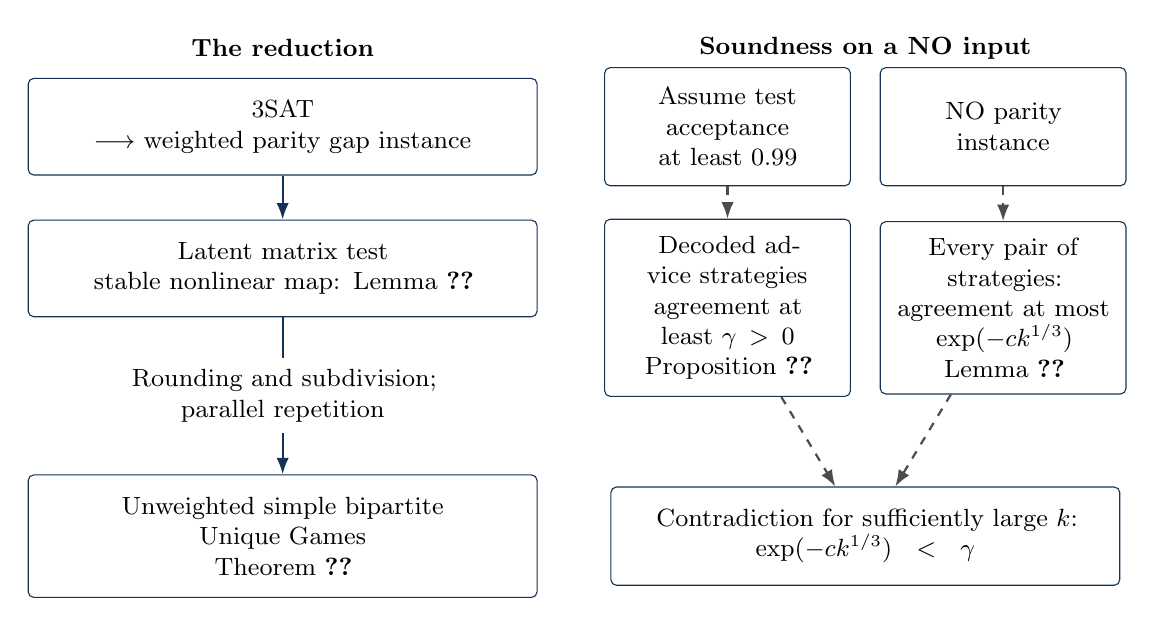
\begin{tikzpicture}[
  x=1cm,y=1cm,
  every node/.style={font=\small},
  box/.style={draw=linkblue!80!black,rounded corners=2pt,
    text width=5.9cm,align=center,inner sep=8pt,minimum height=11mm},
  branch/.style={box,text width=2.70cm,inner sep=6pt,minimum height=15mm},
  heading/.style={font=\small\bfseries,align=center},
  reduction/.style={-{Latex[length=2.1mm]},thick,draw=linkblue!80!black},
  implication/.style={-{Latex[length=2.1mm]},thick,dashed,draw=black!70}
]
\node[heading] at (0,0) {The reduction};
\node[heading] at (7.4,0) {Soundness on a NO input};

\node[box] (parity) at (0,-1.0)
  {$\mathrm{3SAT}$\\$\longrightarrow$ weighted parity gap instance};
\node[box] (matrix) at (0,-2.8)
  {Latent matrix test\\
   stable nonlinear map: Lemma~\ref{lem:latent}};
\node[box] (ugc) at (0,-6.2)
  {Unweighted simple bipartite\\Unique Games\\
   Theorem~\ref{thm:ugc}};
\draw[reduction] (parity) -- (matrix);
\draw[reduction] (matrix) -- node[midway,fill=white,inner sep=4pt,
    text width=5.0cm,align=center]
  {Rounding and subdivision;\\parallel repetition} (ugc);

\node[branch] (assumption) at (5.65,-1.0)
  {Assume test acceptance\\at least $0.99$};
\node[branch] (no) at (9.15,-1.0)
  {NO parity\\instance};
\node[branch] (decoding) at (5.65,-3.3)
  {Decoded advice strategies\\agreement at least $\gamma>0$\\
   Proposition~\ref{prop:matrix-decoding}};
\node[branch] (clean) at (9.15,-3.3)
  {Every pair of\\strategies:\\agreement at most\\$\exp(-c k^{1/3})$\\
   Lemma~\ref{lem:clean}};
\node[box] (contradiction) at (7.4,-6.2)
  {Contradiction for sufficiently large $k$:\\
   $\exp(-c k^{1/3})<\gamma$};
\draw[implication] (assumption) -- (decoding);
\draw[implication] (no) -- (clean);
\draw[implication] (decoding) -- (contradiction);
\draw[implication] (clean) -- (contradiction);
\end{tikzpicture}
\caption{The solid arrows describe the reduction; the dashed arrows describe
its soundness argument. The decoding lower bound follows from high test
acceptance, while the clean-coordinate upper bound follows from the NO
parity gap and applies to every advice strategy. The constants
$c,\gamma>0$ are fixed before the tuple length $k$ grows.}
\label{fig:overview}
\end{figure}


Section~\ref{sec:preliminaries} fixes the game and probability conventions.
Section~\ref{sec:latent} constructs the gadget, and
Section~\ref{sec:game} defines the permutation test.
Sections~\ref{sec:matrix} and~\ref{sec:clean} give the two incompatible
bounds on the advice experiment. Section~\ref{sec:finish} completes
the parameter choices and the explicit Unique Games reduction.
Section~\ref{sec:consequences} then derives the approximation consequences
from the completed theorem and the cited reductions.
Appendix~\ref{app:finite-consequences} gives the simple strong-left
formulation and the finite ordering reduction used there.

\FloatBarrier
\section{Conventions}\label{sec:preliminaries}

\paragraph{Weighted games.}
Intermediate instances may have loops, repeated constraint occurrences,
and positive rational weights summing to one. Their value is the maximum
total weight satisfied by a labeling. Occurrences retain separate IDs
even if their constraints coincide. All rational numbers are encoded by
binary numerators and denominators.

A bipartite \emph{projection game} has a question for each vertex on
either side, finite answer sets, and a map from left answers to right
answers on each constraint. A strategy chooses one answer to each
question. Answer sets that depend on the question can be identified
with fixed alphabets of the same size; we use this for the four
satisfying triples of a parity equation. Each prover uses only its own
question. Private or shared randomness independent of the questions
gives a mixture of deterministic strategies and cannot increase value.

The parallel power \(G^{\otimes t}\) samples \(t\) independent
constraint occurrences, sends the ordered question tuples, and accepts
if every coordinate accepts. Answers may depend on the prover's entire
tuple. Repeated question IDs retain separate coordinate positions and
separate local answer copies. This is the ordinary classical product
game used by the repetition theorem.

\paragraph{Binary linear algebra and Fourier analysis.}
Except where a larger field is specified, all vector spaces and maps
are finite-dimensional over \(\F_2\). Write \(\Hom(E,F)\) for the
space of linear maps and \(E^*=\Hom(E,\F_2)\) for the dual. A subspace
\(S\le E^*\) restricts to its image \(S|_K\le K^*\) on a subspace
\(K\le E\); its restriction rank is \(\dim(S|_K)\).

For a real function \(f\) on a binary space \(E\), use normalized
Fourier coefficients
\[
 \widehat f(g)=\E_{x\in E}f(x)(-1)^{g(x)},\qquad
 f(x)=\sum_{g\in E^*}\widehat f(g)(-1)^{g(x)},\qquad
 \sum_g|\widehat f(g)|^2=\E_x|f(x)|^2.
\]
These identities follow because a nonzero linear functional has equally
many zero and one values, so its character has mean zero. The characters
are therefore an orthonormal basis. On a space of matrices, this is
the entrywise pairing with its dual matrix space; we specify tensor
notation when defining the Fourier decoder.

\paragraph{Probability and finite constructions.}
Uniform sampling from a vector space includes zero. Samples are
independent unless a dependence is stated. For finite probability laws,
\[
 \TV(P,Q)=\frac12\sum_x|P(x)-Q(x)|.
\]
It bounds the difference of expectations of any \([0,1]\)-valued
function. We condition only on events of positive probability.

Random experiments describe finite weighted constraint lists.
The reduction enumerates those lists deterministically. Every auxiliary
dimension and tuple length is fixed before the input formula varies;
the final proof checks both this parameter order and the binary
encoding cost. Fourier witnesses and decoders are used only to bound
game value and need not be efficient.

\section{A latent alphabet gadget}\label{sec:latent}

The construction in this section separates a nonlinear observable from families
of linear observables under the same additive noise.  All vector spaces and
duals in this section are over $\F_2$, unless a different field is indicated.
Restriction of a subspace of a dual means its image under the restriction map.

\begin{lemma}[Latent alphabet gadget]\label{lem:latent}
For every $p_*>0$ there is an integer $r_*$ such that, for every sufficiently
large integer $\ell$, the following objects exist: a finite-dimensional binary
space $\mathcal V$ containing an identified subspace $K=\F_2^\ell$, a map
$C:\mathcal V\to K$, and a rational probability distribution $\mu$ on
$\mathcal V$.  They satisfy
\begin{equation}\label{eq:latent-equivariance}
 C(x+k)=C(x)+k
 \qquad(x\in\mathcal V,\ k\in K),
\end{equation}
and, for independent uniform $x\in\mathcal V$ and $a\sim\mu$,
\begin{equation}\label{eq:latent-small-change}
 \Pr[C(x+a)\ne C(x)]\le p_*.
\end{equation}
Moreover, every linear subspace $G\le\mathcal V^*$ with
$\dim(G|_K)\ge r_*$ satisfies
\begin{equation}\label{eq:latent-detection}
 \Pr_{a\sim\mu}[\text{there exists }g\in G\text{ with }g(a)\ne0]
 \ge\frac18.
\end{equation}
In particular, $r_*$ is fixed before $\ell$ is chosen.
For rational $p_*$, the threshold and all the finite data can be found by a
terminating deterministic algorithm.
\end{lemma}

We first construct a gadget with a fixed smaller output space $B$, in which
shifts induce translations of $B$.  After identifying shifts that induce
the same translation, this gadget will detect every linear family whose
restrictions fill $B^*$.  We then combine copies indexed by injections
$B\to K$: a sufficiently high-rank family on $K$ restricts onto all of
$B^*$ on most copies.  This second step allows every sufficiently large
dimension of $K$ while keeping the rank threshold fixed.

The fixed-$B$ construction begins with a quadratic block.  On an independent
uniform input, a uniform nonzero perturbation in one of its update spaces
leaves the nonlinear output unchanged with probability $\theta$.  A
suitably generic rank-$r$ family of linear observations loses at most one
dimension on the same update space, and a uniform choice of that space
causes a loss with
probability at most $3r\theta$.  A harmonic potential converts this into an
expected loss of at most $3\theta$ per level.  Random changes of coordinates
make nongeneric families rare as they descend, even when later linear maps
depend on earlier choices.
Concatenation therefore makes the nonlinear change probability small while
leaving a constant probability of positive rank.  At the final leaf, a
surviving family detects an independent uniform symbol with constant
probability.

\subsection{The quadratic block}

Fix an integer $r_0\ge1$, whose size will eventually depend only on $p_*$.
Write $H_0=0$ and $H_r=\sum_{j=1}^r 1/j$.  Let
$F=\F_{2^d}$, $q=2^d$, and regard $X=B=F^3$ as binary spaces, each of
dimension $b=3d$.  The integer $d$ will be chosen sufficiently large in terms
of $r_0$.

Use the trace pairing to identify both $X^*$ and $B^*$ with $F^3$:
the vector $z\in F^3$ represents the character
$y\mapsto\operatorname{Tr}_{F/\F_2}(z\cdot y)$, where the dot denotes the
field dot product.  We abbreviate the trace by $\operatorname{Tr}$.
The trace pairing is nondegenerate, and
$\operatorname{Tr}(t^2)=\operatorname{Tr}(t)$.  Every element of $F$ has a
unique square root.

Define
\begin{equation}\label{eq:latent-quadratic}
 Q(x_1,x_2,x_3)=(x_2x_3,x_1x_3,x_1x_2),
 \qquad
 D(x,a)=Q(x+a)+Q(x)+Q(a).
\end{equation}
The block observable is
\[
 C_{\mathrm{blk}}:X\oplus B\longrightarrow B,
 \qquad C_{\mathrm{blk}}(x,y)=y+Q(x).
\]
It is equivariant under the vertical copy of $B$:
$C_{\mathrm{blk}}(x,y+k)=C_{\mathrm{blk}}(x,y)+k$.
For $z\in B^*$, the scalar observation $z\circ C_{\mathrm{blk}}$ changes
by $z(k)$ under this shift.  We shall compare it with linear functionals
whose restriction to the vertical $B$ is also $z$.

For a one-dimensional $F$-subspace $A=Fv$ of $F^3$, put
\begin{equation}\label{eq:latent-block-subspaces}
 D_A=\{y\in B:v\cdot y=0\},
 \qquad
 U_A=\{(a,Q(a)+w):a\in A,\ w\in D_A\}\subseteq X\oplus B.
\end{equation}
These definitions are independent of the chosen nonzero generator $v$.
There are $q^2+q+1$ such lines; set
\begin{equation}\label{eq:latent-theta}
 \theta=\frac{1}{q^2+q+1}.
\end{equation}

\begin{lemma}\label{lem:latent-block}
For every line $A$, the space $U_A$ is binary linear of dimension $b$.
For $a\in A$ and $x\in X$, one has $D(x,a)\in D_A$; for $a,a'\in A$,
one has $D(a,a')=0$.  The trace annihilator of $D_A$ in $B^*=F^3$ is $A$,
and the spaces $U_A$ together span $X\oplus B$.
\end{lemma}

\begin{proof}
The three coordinates of $D(x,a)$ are
\[
 x_2a_3+a_2x_3,\qquad
 x_1a_3+a_1x_3,\qquad
 x_1a_2+a_1x_2.
\]
When $a=tv$, every term in $v\cdot D(x,a)$ occurs twice, so their sum is
zero.  When both arguments are multiples of $v$, each coordinate of the
polar expression is zero.  Thus $Q|_A$ is binary additive, and the
parametrization of $U_A$ by $A\oplus D_A$ is a binary linear bijection.
Its dimension is $d+2d=b$.

Every $z\in A$ annihilates $D_A$ under the trace pairing.  The annihilator
has binary dimension $3d-2d=d$, so it is exactly $A$.
Finally, for each coordinate line $A=Fe_i$, the space $U_A$ contains
$(Fe_i,0)$, because $Q(te_i)=0$, as well as $\{0\}\oplus D_A$.
These three coordinate lines and their vertical hyperplanes span
$X\oplus B$.
\end{proof}

\paragraph{The nonlinear response.}
The form of $U_A$ makes the quadratic term of an update cancel.  For
$(a,Q(a)+w)\in U_A$,
\[
 C_{\mathrm{blk}}\bigl((x,y)+(a,Q(a)+w)\bigr)
       +C_{\mathrm{blk}}(x,y)
 =w+D(x,a).
\]
The right-hand side lies in $D_A$ by Lemma~\ref{lem:latent-block}.
The following calculation gives the exact law that the recursion will use.

\begin{lemma}[Response to one block update]\label{lem:latent-block-noise}
Fix a line $A$.  For independent uniform $(x,y)\in X\oplus B$ and
$\zeta\in U_A\setminus\{0\}$,
\[
 \Pr\bigl[C_{\mathrm{blk}}((x,y)+\zeta)
             \ne C_{\mathrm{blk}}(x,y)\bigr]=1-\theta.
\]
\end{lemma}

\begin{proof}
First take $\zeta$ uniform in all of $U_A$, still independently of the
uniform aggregate.  Its parametrization
$(a,Q(a)+w)$ has independent uniform $a\in A$ and $w\in D_A$.
For every fixed $x,a$, the output difference $w+D(x,a)$ is uniform in
$D_A$, so it is nonzero with probability $1-q^{-2}$.  The zero
perturbation has mass $q^{-3}$ and never changes the output.  Conditioning
on a nonzero perturbation therefore gives
\[
 \frac{1-q^{-2}}{1-q^{-3}}
 =\frac{q(q+1)}{q^2+q+1}=1-\theta.
\]
\end{proof}

The lemma concerns an independent uniform aggregate and uniform nonzero
update.  When the update comes from a lower level of the recursion, we will
verify this conditional law before applying the lemma.

\paragraph{Linear restrictions.}
Fix a binary subspace $S\le B^*$.  A linear functional on $X\oplus B$
whose restriction to the vertical $B$ is $z\in S$ has a unique form
$(\gamma_z,z)\in X^*\oplus B^*$.  Thus a binary-linear choice of one such
extension for each $z\in S$ is specified by a binary linear map
$\gamma:S\to X^*$.  We ask which of these chosen extensions vanish when
restricted to $U_A$.  The restriction loses rank exactly when its kernel
contains a nonzero element.

\begin{lemma}[Kernel of a block restriction]\label{lem:latent-block-kernel}
Let $S\le B^*$ and let $\gamma:S\to X^*$ be binary linear.  For each line
$A$, define
\[
 \kappa_{A,\gamma}:S\longrightarrow U_A^*,
 \qquad \kappa_{A,\gamma}(z)=(\gamma_z,z)|_{U_A}.
\]
Under the trace identification, write
$\gamma_z(x)=\operatorname{Tr}(g(z)\cdot x)$ for the associated binary
linear map $g:S\to F^3$.  For every nonzero $z\in S$,
\[
 \kappa_{A,\gamma}(z)=0
 \quad\Longleftrightarrow\quad
 A=Fz
 \quad\text{and}\quad
 z\cdot g(z)=\sqrt{z_1z_2z_3}.
\]
\end{lemma}

\begin{proof}
If $z$ lies in the kernel, it annihilates every vertical vector
$(0,w)$ with $w\in D_A$.  Lemma~\ref{lem:latent-block} therefore gives
$z\in A$, and for $z\ne0$ this means $A=Fz$.  On the remaining vectors
$(tz,Q(tz))$, $t\in F$, the functional has value
\begin{equation}\label{eq:latent-kernel-trace}
 \operatorname{Tr}\bigl(t\,g(z)\cdot z+t^2z_1z_2z_3\bigr).
\end{equation}
The three summands of $z\cdot Q(tz)$ are equal, and three equals one in
characteristic two.  Also
\[
 \operatorname{Tr}(t^2c)=\operatorname{Tr}(t\sqrt c).
\]
Nondegeneracy of the trace pairing shows that
Equation~\eqref{eq:latent-kernel-trace} vanishes for every $t$ exactly when
$z\cdot g(z)=\sqrt{z_1z_2z_3}$.  Together with $z\in A$, this condition
is sufficient as well: the vertical part is already annihilated.
\end{proof}

\subsection{Generic spaces of characters}

The kernel criterion suggests two sufficient controls.  We shall use a
family in which no field line contains two nonzero characters and only a few
characters satisfy the alignment equation for any one choice of extensions.
The uniformity over that choice will later allow a lift to depend on earlier
random changes of coordinates.

\begin{definition}
A binary subspace $S\le F^3$ of dimension $r\ge1$ is \emph{generic} if
no two distinct nonzero elements of $S$ are proportional over $F$, and if,
for every binary linear map $g:S\to F^3$, at most $3r$ nonzero $z\in S$
satisfy
\begin{equation}\label{eq:latent-alignment}
 z\cdot g(z)=\sqrt{z_1z_2z_3}.
\end{equation}
\end{definition}

Fix one map $\gamma:S\to X^*$ before choosing a uniform line $A$, and let
$r_A=\dim\im\kappa_{A,\gamma}$, where $r=\dim S>0$.
Lemma~\ref{lem:latent-block-kernel} now bounds the loss.  If $S$ is generic,
each field line contains at most one nonzero element of $S$, so the kernel
has dimension at most one.  For the fixed map $g$ associated with
$\gamma$, at most $3r$ characters satisfy Equation~\eqref{eq:latent-alignment};
hence at most $3r$ lines can cause any rank loss.  Consequently
\begin{equation}\label{eq:latent-generic-rank-loss}
 r-r_A\le1,\qquad
 \Pr_A[r_A<r]\le3r\theta,\qquad
 \E_A[H_r-H_{r_A}]\le3\theta.
\end{equation}
The last bound uses $H_r-H_{r-1}=1/r$.
For an arbitrary rank-$r$ space, a loss still requires $A=Fz$ for some
nonzero $z\in S$.  Therefore
\begin{equation}\label{eq:latent-arbitrary-rank-loss}
 \Pr_A[r_A<r]\le(2^r-1)\theta\le2^r\theta,
 \qquad H_r-H_{r_A}\le H_r.
\end{equation}
These estimates concern rank under restriction.  Detection of the eventual
noise will follow only after a positive-rank family reaches a leaf.

It remains to show that spaces with the stated genericity are abundant.

\begin{lemma}\label{lem:latent-generic}
For each fixed $r\ge1$, a uniformly random binary $r$-dimensional subspace
of $F^3$ is generic with probability tending to one as $d\to\infty$.
\end{lemma}

\begin{proof}
Choose independent uniform $x_{ij}\in F$, for $1\le i\le3$ and
$1\le j\le r$, and parametrize a binary linear map by
\[
 z_i(t)=\sum_{j=1}^r x_{ij}t_j,
 \qquad t\in\F_2^r.
\]
Each nonzero input has uniform image in $F^3$, so the probability that this
map is not injective is at most $(2^r-1)q^{-3}$.  Conditioned on
injectivity, its image is a uniform binary $r$-subspace: every such
subspace has the same number of ordered binary bases.  Distinct nonzero
binary inputs are linearly independent also over $F$, so their images are
independent uniform elements of $F^3$.  A union bound therefore shows that
the nonproportionality condition fails with probability $O_r(q^{-2})$,
apart from the event of noninjectivity.

It remains to prove the alignment condition simultaneously for all $g$.
Fix a set $E$ of more than $3r$ distinct nonzero inputs in $\F_2^r$.
On an injective parametrization, the values of a binary linear $g$ on a
basis can be arbitrary vectors in $F^3$.  Thus alignment on all of $E$
implies that the vector
\[
 c=\bigl(\sqrt{z_1(t)z_2(t)z_3(t)}\bigr)_{t\in E}
\]
lies in the $F$-column span of the matrix with $3r$ columns
\[
 M_{t,(i,j)}=t_jz_i(t),
 \qquad t\in E,\quad 1\le i\le3,\quad 1\le j\le r.
\]
Conversely, membership supplies the basis values of such a $g$.
In particular, this column-membership condition already accounts for all
possible maps $g$.

First regard the $x_{ij}$ as independent indeterminates and set
$L=\F_2(x_{ij})$.  We claim that $c$ is not in the column span of $M$ even
after extending scalars to an algebraic closure $\overline L$.
The following $r^3$ elements are linearly independent over $L$:
\[
 \sqrt{x_{1j}x_{2k}x_{3l}},
 \qquad 1\le j,k,l\le r.
\]
Indeed, after clearing denominators, a dependence would be a polynomial
identity in the square roots of the
indeterminates.  The displayed monomials have distinct parity vectors,
whereas coefficients polynomial in the $x_{ij}$ have even exponents in
those square roots.  Terms from different parity vectors cannot cancel.

The expansion of $c$ in these independent elements has coefficient vectors
\[
 v_{jkl}=(t_jt_kt_l)_{t\in E}.
\]
Suppose that $c$ belonged to the column span over $\overline L$.
Every row vector over $L$ annihilating $M$ would then annihilate $c$.
The independence just proved implies that it would annihilate every
$v_{jkl}$.  By double annihilation in the finite-dimensional space
$L^E$, every $v_{jkl}$ would belong to the column span over $L$ itself.

For $h\ge1$, let $V_h\le L^E$ be the evaluation span of all
positive-degree monomials in the binary coordinates $t_1,\ldots,t_r$
of degree at most $h$.  Repeated indices in $v_{jkl}$ give all monomials
of degrees one and two as well as three, because $t_i^2=t_i$ on the
evaluation set.  The preceding conclusion and the form of the columns
therefore imply
\[
 V_3\subseteq\operatorname{col}_L(M)\subseteq V_2\subseteq V_3.
\]
These three spaces are equal.  Multiplication by any $t_i$ sends $V_2$
into $V_3$, so preserves their common value.  Since this space contains
the degree-one monomials, it contains evaluations of every positive-degree
monomial.  These evaluations span all of $L^E$: for any nonzero binary
point, its usual indicator polynomial is a product of factors $t_i$ and
$1+t_i$ with at least one factor $t_i$, and thus has no constant monomial.
Its restriction to $E$ gives the corresponding point indicator.
Consequently the column span would have dimension $|E|>3r$, a
contradiction.

To pass from this algebraic statement to finite fields, square the entries
of both $M$ and $c$.  The resulting matrices have polynomial entries,
and the appended column has entries $z_1(t)z_2(t)z_3(t)$.
Let $h=\rank_L M\le3r$.  Squaring preserves rank over $\overline L$,
so the augmented squared matrix has a nonzero minor of size $h+1$.
This minor is a nonzero polynomial of degree at most $2h+3\le6r+3$.
All unaugmented minors of size $h+1$ vanish identically, so the
unaugmented rank cannot increase on specialization.  It follows that
specialized column membership forces this particular nonzero polynomial
to vanish.  For uniform independent $x_{ij}\in F$, this event has
probability at most $(6r+3)/q$ by the polynomial zero bound~\cite[Corollary~1]{Schwartz80};
see also the earlier sparse-polynomial formulation in~\cite[Section~3.1]{Zippel79}.

If the alignment condition fails, it fails on some set $E$ of size
$3r+1$.  There are finitely many such sets depending only on $r$; if
$2^r-1\le3r$ there are none and the condition is automatic.  A union
bound, followed by conditioning on injectivity, proves the lemma.
\end{proof}

Genericity therefore controls every possible map $g$.  We now fix a
field where nongeneric spaces are rare at every rank up to $r_0$; no linear
maps need to be chosen at this stage.  Choose a positive $\eps_0$ with
\begin{equation}\label{eq:latent-generic-error}
 H_{r_0}2^{r_0}\eps_0\le1,
 \qquad \eps_0<1.
\end{equation}
By Lemma~\ref{lem:latent-generic}, we may fix $d$ sufficiently large that
$b=3d\ge r_0$ and, for every $1\le r\le r_0$, a uniform rank-$r$
subspace of $B^*$ is nongeneric with probability at most $\eps_0$.
In particular, there exists a generic rank-$r_0$ subspace, which we fix
once and for all.

\subsection{Concatenation and its noise}

We keep the output space $B$ fixed while concatenating the quadratic blocks.
One noisy branch will be chosen at each level.  The next lemma computes how
fast the nonlinear change probability decays; we will then track the rank
of linear restrictions along the same branch.

We construct binary input spaces $P_t$, shift subspaces $R_t\le P_t$,
linear surjections $\lambda_t:R_t\to B$, and maps $C_t:P_t\to B$ such that
\begin{equation}\label{eq:latent-recursive-equivariance}
 C_t(u+h)=C_t(u)+\lambda_t(h)
 \qquad(h\in R_t).
\end{equation}
A shift $h\in R_t$ thus represents the output translation $\lambda_t(h)$;
different shifts may represent the same translation.  This form of the
shift action is preserved by aggregation.  At the end, quotienting by the
shifts of value zero will turn the output translations into an actual
subspace of the input.

At height zero take $P_0=R_0=B$ and $C_0=\lambda_0=\operatorname{id}_B$.
Let $\mathcal I$ consist of all pairs $(A,J)$, where $A$ is a line in
$F^3$ and $J:B\to U_A$ is a binary linear isomorphism.  Each line has
the same number of such isomorphisms.

We include one child for every $(A,J)$ in a single fixed parent map.
Choosing a uniform noisy child will then sample a uniform line and a fresh
uniform isomorphism.
For $t\ge1$, take $P_t=\prod_{(A,J)\in\mathcal I}P_{t-1}$ and set
\begin{equation}\label{eq:latent-recursive-output}
 (x,y)=\sum_{A,J}J C_{t-1}(u_{AJ}),
 \qquad C_t(u)=C_{\mathrm{blk}}(x,y)=y+Q(x).
\end{equation}
A tuple of child shifts changes this aggregate by the sum of their embedded
output translations.  To make the parent change a pure output translation,
we require the $X$-component of this sum to vanish.  Accordingly, define
\begin{equation}\label{eq:latent-recursive-shifts}
 R_t=\left\{(h_{AJ})\in\prod_{A,J}R_{t-1}:
       \sum_{A,J}J\lambda_{t-1}(h_{AJ})\in\{0\}\oplus B\right\},
\end{equation}
and let $\lambda_t(h)=k$ when this aggregate is $(0,k)$.
These are linear definitions, and Equation~\eqref{eq:latent-recursive-equivariance}
follows immediately from Equation~\eqref{eq:latent-recursive-output}.
Surjectivity follows inductively from Lemma~\ref{lem:latent-block}: the
child output translations can be chosen arbitrarily, and their aggregate map
is onto $X\oplus B$.
Equation~\eqref{eq:latent-recursive-equivariance} and surjectivity also show
that $C_t$ sends a uniform input to a uniform element of $B$.

Let $\xi_t$ be the following additive noise in $P_t$.
At height zero it is uniform in $B$.  At a positive height, choose a
uniform child $(A,J)$ and embed an independent copy of $\xi_{t-1}$ in
that child, with zero in all other children.  Equivalently, choose a
uniform leaf in the product tree and add a uniform symbol of $B$ at that
leaf.  Each path choice can be sampled as a uniform $A$ followed by a
uniform $J$, independently at successive levels.  All these distributions
are rational. Figure~\ref{fig:latent-recursion} illustrates one level
of the recursion and the selected noisy branch.
\begin{figure}[!htbp]
\centering
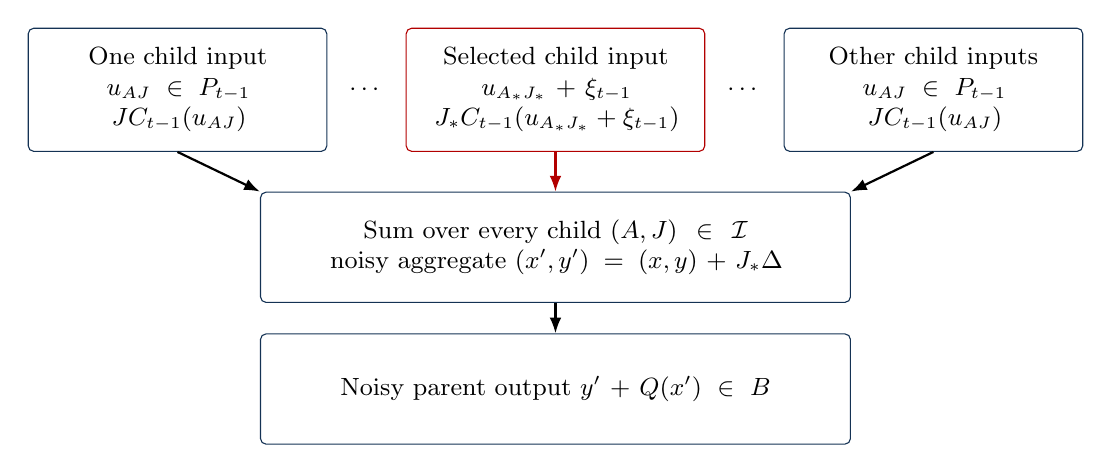
\begin{tikzpicture}[
 every node/.style={font=\small,align=center},
 block/.style={draw=linkblue!80!black,rounded corners=2pt,
 text width=3.3cm,inner sep=7pt,minimum height=14mm},
 flow/.style={-{Latex[length=2mm]},thick}]
\node[block] (left) at (0,0)
 {One child input\\$u_{AJ}\in P_{t-1}$\\$J C_{t-1}(u_{AJ})$};
\node[block,draw=red!70!black] (selected) at (4.8,0)
 {Selected child input\\$u_{A_*J_*}+\xi_{t-1}$\\$J_*C_{t-1}(u_{A_*J_*}+\xi_{t-1})$};
\node[block] (right) at (9.6,0)
 {Other child inputs\\$u_{AJ}\in P_{t-1}$\\$J C_{t-1}(u_{AJ})$};
\node at (2.4,0) {$\cdots$};
\node at (7.2,0) {$\cdots$};
\node[block,text width=7cm] (sum) at (4.8,-2)
 {Sum over every child $(A,J)\in\mathcal I$\\
 noisy aggregate $(x',y')=(x,y)+J_*\Delta$};
\draw[flow] (left.south) -- (sum.north west);
\draw[flow,draw=red!70!black] (selected) -- (sum);
\draw[flow] (right.south) -- (sum.north east);
\node[block,text width=7cm] (out) at (4.8,-3.8)
 {Noisy parent output $y'+Q(x')\in B$};
\draw[flow] (sum) -- (out);
\end{tikzpicture}
\caption{One level of the latent recursion, shown under its additive noise.
The input space is a product over all child indices $(A,J)$; only one
uniformly chosen child is perturbed. Each child output is embedded in
$U_A\le X\oplus B$, all embedded outputs are added, and the quadratic
map is applied once at the parent. Here $(x,y)$ is the initial aggregate,
and $\Delta$ is the selected child's output difference, so the noisy
aggregate is $(x',y')=(x,y)+J_*\Delta$. The omitted children obey the
same rule. The highlighted perturbation may disappear at the parent.}
\label{fig:latent-recursion}
\end{figure}

\FloatBarrier

\begin{lemma}\label{lem:latent-noise}
For independent uniform $u\in P_t$ and noise $\xi_t$,
\begin{equation}\label{eq:latent-change-probability}
 p_t:=\Pr[C_t(u+\xi_t)\ne C_t(u)]
     =(1-q^{-3})(1-\theta)^t.
\end{equation}
\end{lemma}

\begin{proof}
The identity at height zero is immediate.  Consider one higher level and
condition on the selected child $(A,J)$.  Write $\Delta$ for its output
difference.  All child copies have the same function and the same inner
noise law, so the law of $\Delta$ is independent of the selected index.

We need also the conditional law of the child's initial output.
For any fixed child perturbation $a$, Equation~\eqref{eq:latent-recursive-equivariance}
gives
\[
 C_{t-1}(u+a+h)+C_{t-1}(u+h)
 =C_{t-1}(u+a)+C_{t-1}(u)
 \qquad(h\in R_{t-1}).
\]
Thus the difference is invariant under these shifts, while the initial
output is translated by every element of $B$.  On uniform input its
initial output remains uniform conditional on the difference, even if the
inner perturbation is also specified.  All other initial child outputs
remain independently uniform.  Because the aggregate map is onto
$X\oplus B$, the initial aggregate $(x,y)$ is therefore uniform
conditional on $(A,J,\Delta)$.  In particular it is independent of the
aggregate perturbation $J\Delta$.

Conditional on $\Delta\ne0$ and $A$, the isomorphism $J$ remains uniform,
because the law of $\Delta$ is independent of the selected child index.
Thus $J\Delta$ is uniform in $U_A\setminus\{0\}$.  The conditional
uniformity just proved makes the initial aggregate independent of this
update.  Lemma~\ref{lem:latent-block-noise} therefore gives parent change
probability $1-\theta$ conditional on a nonzero child difference.  When
$\Delta=0$, the aggregate does not change.  Consequently
$p_t=p_{t-1}(1-\theta)$, proving the identity.
\end{proof}

\subsection{Linear lifts and loss of rank}

The nonlinear change probability now decays with the height.  For the
fixed-$B$ gadget, our remaining target is detection whenever a family's
restrictions fill $B^*$.  We will prove this by tracking every binary-linear
choice of extensions of these output characters through the shift action.

For $S\le B^*$, a \emph{lift} on $P_t$ means a binary linear map
$z\mapsto\psi_z$ from $S$ to $P_t^*$ satisfying
\begin{equation}\label{eq:latent-lift-definition}
 \psi_z|_{R_t}=z\circ\lambda_t.
\end{equation}
A lift is \emph{full} when its domain is $B^*$.  We next describe every
possible lift at a parent, without making any assumption about how it was
chosen.

\begin{lemma}\label{lem:latent-lift-factorization}
Let a lift with domain $S$ be given on $P_t$, where $t\ge1$.
For each child $(A,J)$, restriction to that child's shift space factors
through $\lambda_{t-1}$.  The resulting characters on the child output
space $B$ have the form
\begin{equation}\label{eq:latent-child-characters}
 \phi_{AJ}(z)=J^*\bigl((\gamma_z,z)|_{U_A}\bigr)\in B^*,
\end{equation}
where $\gamma:S\to X^*$ is a single binary linear map common to all the
children.
\end{lemma}

\begin{proof}
A shift supported on one child and lying in $\ker\lambda_{t-1}$ is a
parent shift with output translation zero.  Each $\psi_z$ vanishes on it,
proving the first assertion.

Let $T=\prod_{A,J}B$ be the space of child output translations, with aggregate
map $\mathcal A:T\to X\oplus B$.  This map is onto.  The sum of the
child characters, minus $z$ applied to the second component of
$\mathcal A$, vanishes whenever the first component of $\mathcal A$ is
zero: every such tuple of translations can be supplied by child shifts,
giving a parent shift.  The difference therefore factors uniquely through the
first component of $\mathcal A$, which is onto $X$.  Call this character
$\gamma_z$.  Uniqueness shows that $\gamma_z$ depends linearly on $z$.
Evaluating on a tuple supported at one child gives
Equation~\eqref{eq:latent-child-characters}.
\end{proof}

After choosing a child, let $S'=\im\phi_{AJ}$ and choose a linear section
$\iota:S'\to S$ of $\phi_{AJ}$.  Restricting $\psi_{\iota(z')}$ to that
child input gives a lift with domain $S'$ on $P_{t-1}$.
We may fix deterministic rules for all such sections.  In particular they
depend only on the already chosen path, and never on a future path index
or on the final noise symbol.  On descending the tree, every surviving
functional is a restriction of a member of the original linear family.

The factorization now connects the recursion to the local restriction
problem.  For a fixed parent lift, its single map $\gamma$ is common to
every outgoing line $A$, and
$\phi_{AJ}=J^*\kappa_{A,\gamma}$.  Since $J^*$ is an isomorphism, it does
not change the kernel or rank.  We may therefore apply
Equations~\eqref{eq:latent-generic-rank-loss}
and~\eqref{eq:latent-arbitrary-rank-loss} when the outgoing line is chosen
uniformly.  The next proof shows that the incoming isomorphisms make
genericity typical at each positive subsequent rank, even though the lift
itself depends on the earlier path.

\begin{proposition}\label{prop:latent-full-lift-detection}
Set
\begin{equation}\label{eq:latent-depth}
 s=\left\lfloor\frac{H_{r_0}}{8\theta}\right\rfloor.
\end{equation}
Every full lift on $P_s$ detects $\xi_s$ with probability at least $1/4$:
\begin{equation}\label{eq:latent-full-lift-detection}
 \Pr[\text{there exists }z\in B^*\text{ with }\psi_z(\xi_s)\ne0]
 \ge\frac14.
\end{equation}
\end{proposition}

\begin{proof}
Restrict the full lift at the top to the fixed generic subspace of
dimension $r_0$.  Follow the random leaf path, replacing the lift at each
chosen child by the image lift just described.  Let $S_j$ be its domain
after $j$ steps, and let $r_j=\dim S_j$, so initially $r_j=r_0$ at $j=0$.
Continue with the zero space after extinction.

We spell out the conditioning that permits genericity to be used at every
level.  Let $\mathcal F_j$ be the information in all path choices before
the outgoing choice $(A_j,J_j)$ at step $j$.  The current space, lift,
and map $\gamma_j$ are $\mathcal F_j$-measurable.
Conditional on $\mathcal F_j$ and $A_j$, the subspace
\[
 E_{j,A_j}
 =\im\bigl[z\mapsto(\gamma_{j,z},z)|_{U_{A_j}}\bigr]
 \le U_{A_j}^*
\]
is fixed.  The next domain and its rank are
\[
 S_{j+1}=J_j^*E_{j,A_j},
 \qquad r_{j+1}=\dim E_{j,A_j}.
\]
The rank is fixed before $J_j$ is revealed.  A uniform binary
isomorphism $J_j:B\to U_{A_j}$ makes $S_{j+1}$ a uniformly random
subspace of $B^*$ of that rank.  Therefore, if $B_j$ is the indicator
that $r_j>0$ and $S_j$ is nongeneric, then
\begin{equation}\label{eq:latent-fresh-orientation}
 \E[B_{j+1}\mid\mathcal F_j,A_j]\le\eps_0.
\end{equation}
The next lift may depend on $J_j$.  This causes no restriction on the
argument: genericity bounds every binary linear map $g$ on the selected
subspace, including the map supplied by that lift.

Let $\Delta_j=H_{r_j}-H_{r_{j+1}}\ge0$.
Conditional on $\mathcal F_j$, the outgoing $A_j$ is independent and
uniform, and the rank-loss estimates above apply to the fixed current
lift.  Consequently
\begin{equation}\label{eq:latent-conditional-harmonic}
 \E[\Delta_j\mid\mathcal F_j]
 \le3\theta+H_{r_0}2^{r_0}\theta B_j.
\end{equation}
For $j=0$ the space is generic, so its expected drop is at most
$3\theta$.  For $j\ge1$, average Equation~\eqref{eq:latent-conditional-harmonic}
over the preceding isomorphism using
Equation~\eqref{eq:latent-fresh-orientation}.  This gives the unconditional
bound
\[
 \E\Delta_j
 \le\bigl(3+H_{r_0}2^{r_0}\eps_0\bigr)\theta
 \le4\theta.
\]
No independence between an incoming orientation and its subsequent lift
has been assumed.

Summing the expected drops and using Equation~\eqref{eq:latent-depth},
\[
 \E[H_{r_0}-H_{r_s}]\le4s\theta\le\frac{H_{r_0}}2.
\]
Extinction requires a total drop of $H_{r_0}$, so
$\Pr[r_s=0]\le1/2$.  At a leaf, $P_0=R_0=B$ and its lift consists of
the characters themselves.  Conditional on any surviving rank $r_s>0$,
an independent uniform symbol in $B$ is detected with probability
$1-2^{-r_s}\ge1/2$.  Every surviving functional is a restriction of the
original family along the selected leaf, so such a detection implies a
detection by that family of the embedded noise $\xi_s$.  Multiplying the
two bounds proves Equation~\eqref{eq:latent-full-lift-detection}.
\end{proof}

\subsection{Quotients and enlargement}

The fixed-$B$ construction is complete once its shift action is realized
by an actual subspace.  Put
\[
 V_0=P_s/\ker\lambda_s,
\]
where the kernel is taken inside $R_s\le P_s$, and let
$q_0:P_s\to V_0$ be the quotient map.
Equation~\eqref{eq:latent-recursive-equivariance} makes $C_s$ invariant under
this kernel, so it descends to a map $\overline C:V_0\to B$.
The quotient $R_s/\ker\lambda_s$ is identified with $B$ by $\lambda_s$,
giving an inclusion $i_B:B\to V_0$ such that
\[
 q_0(h)=i_B(\lambda_s h)\qquad(h\in R_s).
\]
We henceforth identify this subspace with $B$.  Its shift action satisfies
\[
 \overline C(x+b')=\overline C(x)+b'
 \qquad(b'\in B).
\]
Let $\nu$ be the pushforward of the noise law of $\xi_s$.
Uniform input on $P_s$ pushes to uniform input on $V_0$, so the output
change probability remains $p_s$.

Every linear subspace $G_0\le V_0^*$ whose restriction is all of $B^*$
satisfies
\begin{equation}\label{eq:latent-base-detection}
 \Pr_{a\sim\nu}[\text{there exists }g\in G_0\text{ with }g(a)\ne0]
 \ge\frac14.
\end{equation}
Indeed, choose a linear section $\sigma:B^*\to G_0$ of restriction and
define $\psi_z=q_0^*\sigma(z)=\sigma(z)\circ q_0$.  For $h\in R_s$,
\[
 \psi_z(h)=\sigma(z)(q_0h)=z(\lambda_s h).
\]
Thus this pullback is a full lift.  Moreover,
$\psi_z(\xi_s)=\sigma(z)(q_0\xi_s)$, so detection by the lift is detection
by the chosen section on the pushed-forward noise.
Proposition~\ref{prop:latent-full-lift-detection} gives the bound, and
detection by the section implies detection by $G_0$.

\begin{proof}[Proof of Lemma~\ref{lem:latent}]
Choose $r_0$ sufficiently large that
\[
 \exp(1-H_{r_0}/8)\le p_*.
\]
Then choose $\eps_0$ as in Equation~\eqref{eq:latent-generic-error} and
fix $d$, and hence $b=3d$ and $\theta$, using
Lemma~\ref{lem:latent-generic}.  Construct the height $s$ in
Equation~\eqref{eq:latent-depth} and the quotient $(V_0,B,\overline C,\nu)$
above.  Lemma~\ref{lem:latent-noise} gives
\begin{equation}\label{eq:latent-small-base-change}
 p_s\le(1-\theta)^s
 \le\exp(-\theta s)
 \le\exp(\theta-H_{r_0}/8)
 \le p_*.
\end{equation}
Set $r_*=b+2$.  All choices so far depend only on $p_*$.

We now enlarge the output space.  The point of using random injections
$B\to K$ is that a family of restriction rank at least $b+2$ on $K$
restricts onto all of $B^*$ along most injections.  A copy of the base
gadget for each injection will therefore turn its full-restriction
detection bound into the required high-rank bound.

Fix $\ell\ge b+2$ and write $K=\F_2^\ell$.
Let $\mathcal L$ be the finite set of all binary linear injections
$L:B\to K$.  Take a product $P=\prod_{L\in\mathcal L}V_0$ and define
\[
 \widetilde C((x_L)_L)=\sum_{L\in\mathcal L}L\overline C(x_L).
\]
The product of shift subspaces $T=\prod_L B\le P$ acts on this output
through the linear map
\[
 \Lambda:T\longrightarrow K,
 \qquad \Lambda((b_L)_L)=\sum_L Lb_L.
\]
This map is onto, because every nonzero vector of $K$ is in the image of
some injection $B\to K$.  Quotient by its kernel inside $T$:
\[
 \mathcal V=P/\ker\Lambda.
\]
The map $\widetilde C$ descends to $C:\mathcal V\to K$, and
$T/\ker\Lambda$ identifies with the required shift subspace $K$.
This proves Equation~\eqref{eq:latent-equivariance}.

On $P$, choose a uniform $L\in\mathcal L$ and update only that copy by
an independent sample from $\nu$.  Let $\mu$ be the resulting law after
the quotient.  On uniform product input the output sum changes exactly
when the selected copy's output changes, because $L$ is injective.
Uniform input pushes to uniform input on the quotient, so the change
probability is still $p_s$.  Equation~\eqref{eq:latent-small-base-change}
proves Equation~\eqref{eq:latent-small-change}.  Every noise distribution
used here is obtained from uniform finite choices by pushforward, and
therefore is rational.

It remains to establish detection for an arbitrary
$G\le\mathcal V^*$.  Let $S=G|_K\le K^*$, of dimension $r\ge r_*$.
Pull $G$ back to $P$ and then restrict to its copy of $V_0$ indexed by
$L$; denote the resulting subspace of $V_0^*$ by $G_L$.
Its restriction to that copy's shift subspace $B$ is exactly
\[
 G_L|_B=L^*S.
\]
To see this, a shift $b'\in B$ supported on copy $L$ represents the
shift $Lb'\in K$ in the quotient, so a character restricting to
$z\in S$ evaluates there as $z(Lb')$.

The map $L^*:S\to B^*$ fails to be onto if and only if there is a
nonzero $b'\in B$ with $Lb'\in S^\perp$.  For each such fixed $b'$, a
uniform injection $L$ makes $Lb'$ uniform among the nonzero vectors of
$K$.  Hence
\[
 \Pr_L[Lb'\in S^\perp]
 =\frac{2^{\ell-r}-1}{2^\ell-1}
 \le2^{-r}.
\]
A union bound gives
\[
 \Pr_L[L^*S\ne B^*]
 \le(2^b-1)2^{-r}
 \le2^{b-r}\le\frac14.
\]
On each of the remaining copies,
Equation~\eqref{eq:latent-base-detection} gives detection probability at
least $1/4$ by $G_L$, and thus by $G$ on the embedded noise.
Averaging over the selected copy yields detection probability at least
$\frac34\cdot\frac14=\frac{3}{16}\ge\frac18$, proving
Equation~\eqref{eq:latent-detection}.
The construction works for every $\ell\ge b+2$, with the already fixed
$r_*=b+2$, as required.

For completeness, all choices are effective when $p_*$ is rational.
Choose an integer $m\ge0$ with $2^{-m}\le p_*$ and then choose $r_0$ with
$H_{r_0}\ge8(m+1)$; since $e^{-m}\le2^{-m}$, this ensures the initial
bound on $r_0$.  Choose rational $\eps_0$ satisfying
Equation~\eqref{eq:latent-generic-error}.  For successive integers $d$ with
$3d\ge r_0$, enumerate the binary subspaces of $\F_{2^d}^3$ and the linear
maps in the definition of genericity.  This tests genericity exactly and
computes the fraction of nongeneric spaces at each rank $1,\ldots,r_0$.
Lemma~\ref{lem:latent-generic} ensures that eventually all these fractions
are at most $\eps_0$.  Fix the first such field and a generic rank-$r_0$
space.  The remaining products, isomorphisms, injections, quotients, function
tables, and rational noise laws are obtained by finite enumeration and
binary linear algebra.  This gives the asserted terminating construction.
\end{proof}

\section{The outer questions and the permutation test}
\label{sec:game}

We now use the latent gadget to construct a permutation instance.  Its
vertices encode affine tables on tuples of parity equations.  We identify
two tables exactly when they induce the same affine map on the same retained
coordinates, including the same intercept.  This common representation will
allow us to compare an equation tuple with a sparsely projected tuple in
Section~\ref{sec:matrix}.

\subsection{Weighted parity equations and distinct positions}

A \emph{weighted parity instance} consists of a finite variable set
\(\mathcal X\), a finite nonempty set \(\mathcal E\) of equation
occurrences, and positive rational weights \(\omega_e\) summing to one.
An occurrence is an ordered equation
\[
 x_{v_{e,1}}+x_{v_{e,2}}+x_{v_{e,3}}=b_e,
 \qquad b_e\in\F_2.
\]
Its value is the weighted fraction of equations satisfied, and
\(\OPT(\mathcal E)\) denotes the maximum value.  Different occurrences
have different IDs even if their ordered equations coincide.

\begin{theorem}[Weighted parity gap]
\label{thm:parity}
For every fixed rational \(\xi>0\), there is a deterministic
polynomial-time reduction from Boolean satisfiability to weighted parity
instances, with binary-encoded rational weights, such that
\[
 \begin{array}{ll}
 \textup{YES:}&\OPT(\mathcal E)\ge 1-\xi,\\
 \textup{NO:}&\OPT(\mathcal E)\le \frac12+\xi.
 \end{array}
\]
The running-time polynomial may depend on \(\xi\).
\end{theorem}

This is the gap consequence of H\aa stad's construction in
\cite[Theorem~5.4 and its proof]{Hastad01}.  More specifically, the proof
uses a fixed dyadic verifier error \(\delta>0\), gives completeness
\(1-\delta\) and soundness \((1+\delta)/2\), and enumerates verifier
choices as equations with their rational probabilities as weights.
Choosing \(\delta\le\xi\) gives the displayed statement.  The
enumeration is a deterministic reduction; the verifier's random choices
describe the resulting weighted instance.

\begin{lemma}[Making positions distinct]
\label{lem:distinct-parity}
From a weighted parity instance \(\mathcal E\) one can deterministically
construct, in polynomial time, an instance \(\mathcal E'\) in which the
three variable IDs of every occurrence are distinct.  Its weights are
positive rationals of polynomial bit length, and
\[
 \OPT(\mathcal E')\ge\OPT(\mathcal E),
 \qquad
 \OPT(\mathcal E')
 \le \frac{1+\OPT(\mathcal E)}2+\frac3{100}.
\]
In particular, Theorem~\ref{thm:parity} with \(\xi<1/100\), followed by
this preprocessing, gives completeness at least \(1-\xi\) and NO
optimum at most \(4/5\).
\end{lemma}

\begin{proof}
Replace each variable \(v\) by one hundred clones \((v,c)\),
\(c\in[100]\).  For each original occurrence, choose its three clones
uniformly subject to choosing distinct clones whenever positions have
the same underlying variable.  List all the resulting occurrences and
give them the corresponding conditional weights.  There are at most
\(100^3\) choices per original occurrence.  Giving all clones their
original variable's label proves the completeness assertion.

For the upper bound fix arbitrary clone labels, and let
\[
 t_v=\frac1{100}\sum_{c=1}^{100}(-1)^{x_{(v,c)}}.
\]
First choose clones independently, without conditioning on distinctness.
The satisfaction probability of occurrence \(e\) is
\[
 \frac{1+(-1)^{b_e}t_{v_{e,1}}t_{v_{e,2}}t_{v_{e,3}}}{2}.
\]
Round each bias to a majority label, resolving zero biases arbitrarily.
For every equation violated by this rounded assignment, the signed
product in the numerator is nonpositive, so its satisfaction probability
is at most \(1/2\).  The other equations have probability at most one.
The weighted mean is therefore at most
\((1+\OPT(\mathcal E))/2\).  The probability of a forbidden collision
among the independently chosen clones is at most \(3/100\), by a union
bound over the three pairs of positions.  Conditioning on its complement
changes the expectation of any \([0,1]\)-valued function by at most
\(3/100\).  This proves the bound.  All conditional probabilities have
constant-size denominators apart from their original occurrence weights.
\end{proof}

For the rest of the construction, \(\mathcal E\) denotes the
preprocessed instance, so every equation has three distinct variable
IDs.  Its \emph{ordinary equation-versus-variable game} samples
\(e\) according to \(\omega\) and \(j\) uniformly from \([3]\).
The first prover receives the occurrence ID \(e\) and answers with a
satisfying triple for that equation; the second receives the variable ID
\(v_{e,j}\) and answers with a bit.  Acceptance means equality at
position \(j\).  Because the IDs within an equation are distinct,
the question pair determines the projection constraint.

For any second-prover strategy, its bits constitute a global assignment.
On an equation violated by that assignment, every valid first-prover
answer disagrees in at least one position.  Hence this ordinary
projection game, denoted \(G_{\mathcal E}\), satisfies
\begin{equation}
 \val(G_{\mathcal E})
 \le 1-\frac{1-\OPT(\mathcal E)}3
 \le \frac{14}{15}
 \quad\text{if }\OPT(\mathcal E)\le\frac45.
 \label{eq:base-game-gap}
\end{equation}
The answer alphabets have sizes four and two, respectively.

\subsection{Tuples, local answer copies, and homogeneous coordinates}

Fix a positive integer \(k\).  An equation question
\(U=(e_1,\ldots,e_k)\) is sampled from \(\omega^{\otimes k}\), with
replacement.  Its answer space is the product of the \(k\) affine
solution planes.  Blocks always use local copies: even if the same
equation or variable ID appears in several blocks, their local answers
are separate coordinates.

For a parameter \(0<\beta<1\), independently in every block either
retain the equation, with probability \(1-\beta\), or retain just the
variable ID at a uniformly chosen position, with probability \(\beta\).
The resulting question is denoted \(O\), and \(\pi\) is the
coordinate projection from answers on \(U\) to answers on \(O\).
The question \(O\) records an equation ID or a variable ID at every
ordered block position.  A singleton block accepts either bit.

Represent an equation answer by its first two bits \((x_i,y_i)\);
the third is \(b_{e_i}+x_i+y_i\).  A singleton is represented by its
actual bit.  Add a common homogeneous coordinate \(t_0\).  Thus
\[
 L_U=\F_2^{1+2k},\qquad m=1+2k,
\]
and \(L_O\) has one homogeneous coordinate, two coordinates for each
retained equation, and one for each singleton.  In either space, vectors
whose first coordinate is one are exactly valid answers.  Write
\(e_0^\top\) for the functional reading that coordinate.

The affine projection \(\pi\) extends to a linear surjection
\(\bar\pi:L_U\to L_O\) preserving \(t_0\).  On retained equation
blocks it is the identity, and on a block projected to a singleton its
coordinate is
\begin{equation}
 \begin{cases}
 x_i,&\text{position }1,\\
 y_i,&\text{position }2,\\
 b_{e_i}t_0+x_i+y_i,&\text{position }3.
 \end{cases}
 \label{eq:outer-projection}
\end{equation}
We call every map obtained by these blockwise choices a \emph{permitted
projection}; this class of maps is independent of \(\beta\).
Surjectivity follows by fixing \(t_0\) and choosing coordinates
independently in each block.  We use the same conventions for questions
with some blocks omitted.

\subsection{Exact table keys and folding}

The identification of tables across projected questions follows the
virtual-table approach of Khot--Safra~\cite[Section~1.1]{KS13}.
We first express each table on the coordinates through which it factors.
This will give the same representation to a projected table and its
pullback.

Fix latent data \((\mathcal V,K,C,\mu)\) from
Lemma~\ref{lem:latent}, where \(K=\F_2^\ell\), and fix a linear
complement \(\mathcal V=K\oplus W\).  A \emph{table} on a question
\(Q\) is an affine map from its answer space to \(\mathcal V\), or
equivalently its unique linear extension
\(P\in\Hom(L_Q,\mathcal V)\).  Here \(Q\) may be an equation
question or one of its permitted projections, and the same definition
applies to a question with omitted blocks.  Write \(c\) for the
coefficient of the homogeneous coordinate \(t_0\) in \(P\).

In an equation block, inspect the rank of its slope map
\(\F_2^2\to\mathcal V\), whose contribution we write as
\(a_i x_i+d_i y_i\).  If its rank is two, retain the equation
occurrence and this contribution.  If its rank is zero, omit the block.
In the remaining case the rank is one, so the coefficients have exactly
one of the forms
\[
 (a_i,d_i)=(v,0),\quad (0,v),\quad (v,v),
 \qquad v\ne0.
\]
These forms retain only the variable at position one, two, or three,
respectively, with contribution \(v z_i\) in its actual bit \(z_i\).
For the third form,
\[
 v(x_i+y_i)=v z_i+b_{e_i}v t_0,
 \qquad z_i=b_{e_i}t_0+x_i+y_i,
\]
so this replacement also adds \(b_{e_i}v\) to the homogeneous
intercept.  In a singleton block, retain its variable ID and its original
contribution exactly when its slope is nonzero; otherwise omit the block.

The retained blocks form the \emph{support} of \((Q,P)\).  They keep
their indices in \([k]\), their equation/variable tags, and their IDs.
A retained equation keeps its ordered first two coordinates, and a retained
singleton uses its actual-bit coordinate.  Thus repeated IDs in different
blocks still have separate local coordinates.  The support may be empty;
its homogeneous coordinate remains in every case.

Let \(J_3\) be the set of equation blocks reduced to their third bit,
and write \(v_i\) for the nonzero slope in such a block.  The
\emph{reduced table} \(\widetilde P\) on the support has the retained
block contributions specified above and homogeneous intercept
\begin{equation}
 \widetilde c=c+\sum_{i\in J_3} b_{e_i}v_i.
 \label{eq:reduced-table-intercept}
\end{equation}
To check the complete table, let \(L_{\rm supp}\) be the homogeneous
answer space of the support and let
\(\rho_{Q,P}:L_Q\to L_{\rm supp}\) retain \(t_0\) and the
specified block coordinates.  It is the identity on retained equations
and on retained singleton blocks already present in \(Q\), uses the
corresponding actual-bit coordinate from
Equation~\eqref{eq:outer-projection} on a reduced equation, and discards
omitted blocks.  Choosing the coordinates independently in each
block shows that \(\rho_{Q,P}\) is surjective.  The block identities
and Equation~\eqref{eq:reduced-table-intercept} give
\[
 P=\widetilde P\rho_{Q,P}.
\]
Surjectivity makes \(\widetilde P\) the unique linear map with this
factorization.  We define the \emph{key} of \((Q,P)\) to be its
support together with this entire reduced table.  Thus two tables have
the same key exactly when their retained coordinates agree, with the same
positions, tags, and IDs, and their induced affine maps agree on those
coordinates, including their intercepts.

We next check compatibility with every permitted projection
\(\bar\pi:L_U\to L_O\).  Let
\(P'\in\Hom(L_O,\mathcal V)\).  An equation retained in \(O\)
has the same contribution in \(P'\) and its pullback \(P'\bar\pi\),
so its reduction is identical.  A singleton of slope zero disappears on
both sides.  A singleton of nonzero slope \(v\) pulls back to the
corresponding one of the three rank-one patterns above, which reduces to
the same variable ID at the same block position.  For a third-position
singleton, the pullback adds \(b_{e_i}v\) to the intercept, and its
reduction adds \(b_{e_i}v\) once more.  The two terms cancel over
\(\F_2\).  All other intercept corrections come from retained equation
blocks and are identical on the two sides.  The supports and complete
reduced tables therefore agree: \((U,P'\bar\pi)\) and \((O,P')\)
have the same key.

Define the key universe to consist of the keys of all tables on equation
questions \(U\in\mathcal E^k\).  The compatibility just proved shows
that the key of every table on a permitted projected question already
belongs to this universe, by pullback from any compatible \(U\).

We now apply the folding principle of Bellare, Goldreich, and
Sudan~\cite[Section~3.3]{BGS98}: values on one representative determine
the values on its translates.  Adding a constant \(h\in K\) to a key
means adding \(h\) to its reduced intercept, leaving its support and
slopes fixed.  This is realized by replacing a presenting table \(P\)
with \(P+h e_0^\top\), so it preserves the key universe.  The action
is free because the key records the intercept.  A vertex of our
permutation instance is an orbit of this action, represented by its unique
key whose reduced intercept has zero \(K\) component.

For a table \(P\) on an equation question or a permitted projected
question \(Q\), let \(c(Q,P)\in K\) be the \(K\) component of
its key's reduced intercept.  Let \(v(Q,P)\) denote the orbit vertex
represented by the key obtained after removing this component.
A labeling \(\lambda\) of the vertices defines the restored table answer
\[
 F_Q(P)=\lambda(v(Q,P))+c(Q,P).
\]
Adding a constant changes only the removed component, so
\begin{equation}
 F_Q(P+h e_0^\top)=F_Q(P)+h
 \qquad(h\in K).
 \label{eq:table-folding}
\end{equation}
Tables with the same key have the same representative and removed
component.  The pullback compatibility therefore gives, for every
permitted \(U,O,\bar\pi\) and every table \(P'\) on \(O\),
\begin{equation}
 F_U(P'\bar\pi)=F_O(P').
 \label{eq:key-sharing}
\end{equation}
Projected questions thus use answers determined by the same vertex
labeling, without an additional consistency test.

\subsection{The latent matrix test and completeness}

The permutation instance, denoted \(\mathcal G\), samples independently
\[
 U\sim\omega^{\otimes k},\qquad
 P\text{ uniform in }\Hom(L_U,\mathcal V),\qquad
 a\sim\mu,\qquad l\text{ uniform in }\F_2^m,
\]
and checks
\begin{equation}
 F_U(P)=F_U(P+a l^\top).
 \label{eq:matrix-test}
\end{equation}
Here \(a l^\top\) denotes the map \(z\mapsto a(l^\top z)\).
Each sample specifies an edge between the two key-orbit vertices.  If
their restored offsets are \(c_0,c_1\), its constraint is the
permutation
\[
 \lambda(v_1)=\lambda(v_0)+c_0+c_1
\]
of the fixed alphabet \(K\).  Edge occurrences have their sampling
probabilities as weights.  At this stage loops and repeated edges are
allowed.  The sparse projection experiment involving \(O\) is used to
analyze these same vertex labels; it is not an additional test in
\(\mathcal G\).

\begin{lemma}[Completeness of the outer matrix test]
\label{lem:outer-completeness}
If \(\mathcal E\) has an assignment of value at least \(1-\xi\), and
the latent map satisfies
\[
 \Pr_{x\text{ uniform in }\mathcal V,\ a\sim\mu}
       [C(x+a)\ne C(x)]\le p_*,
\]
then
\[
 \val(\mathcal G)\ge 1-k\xi-\frac{p_*}{2}.
\]
\end{lemma}

\begin{proof}
Fix the near-satisfying global bit assignment.  Give every reduced
support a valid answer as follows.  At a singleton use its global bit.
At a retained equation use its first two global bits and set the third
to the unique value satisfying the equation.  These choices depend only
on the support, including its occurrence IDs, and therefore define an
answer for every exact key independently of its origin.

At an orbit representative, evaluate its reduced table on this answer
and apply \(C\).  This defines a vertex labeling.  The equivariance of
\(C\) under \(K\) implies that its restored answer is evaluation of
the actual reduced table followed by \(C\), in agreement with
Equation~\eqref{eq:table-folding}.

With probability at least \(1-k\xi\), every equation in \(U\) is
satisfied by the global assignment.  On such a tuple, the support
answers used for \emph{every} table are projections of the same full
answer \(z_U\in L_U\), whose first coordinate is one.  Consequently
the two sides of Equation~\eqref{eq:matrix-test} are
\[
 C(Pz_U)\quad\text{and}\quad
 C(Pz_U+a(l^\top z_U)).
\]
Since \(z_U\ne0\), the vector \(Pz_U\) is uniform in
\(\mathcal V\), independently of \(a,l\), and \(l^\top z_U\) is
an independent fair bit.  The test therefore fails with probability at
most \(p_*/2\) on these tuples.  Adding the probability of a tuple
containing an unsatisfied equation proves the bound.
\end{proof}

\section{Matrix extraction and Fourier decoding}
\label{sec:matrix}

We convert high acceptance of the matrix test into agreement between two
strategies for the sparsely projected questions $U,O$.  Each strategy
uses only its own question and a bounded number of rows of matrix advice.
The resulting agreement probability is positive independently of the tuple
length $k$ and the parity instance.  The table functions enter only through
their folding and sharing identities and the acceptance bound, so the proof
applies to any family with these properties; the restored functions of every vertex
labeling are examples.  We state the precise assumptions below, after
fixing the parameters and defining the advice experiment.

\subsection{The inverse shortcode theorem}

The structural input describes functions that often keep their value
under a uniform rank-one perturbation.  Such a function agrees with an
affine evaluation on a set obtained by fixing a bounded number of linear
combinations of rows and columns.

Write $\operatorname{Mat}_{\ell,m}=\Hom(\F_2^m,\F_2^\ell)$.
A \emph{row and column slice} is a nonempty set specified by equations
\begin{equation}
 \mathcal S=
 \{M:d_i^\top M=s_i^\top\ (1\le i\le n_r),\quad
          Mq_j=t_j\ (1\le j\le n_c)\},
 \label{eq:shortcode-slice}
\end{equation}
where $d_i\in\F_2^\ell$, $s_i\in\F_2^m$, $q_j\in\F_2^m$, and
$t_j\in\F_2^\ell$.  The counts $n_r,n_c$ need not be the ranks of their
respective systems.

\begin{theorem}[Equality soundness for degree-two shortcode]
\label{thm:shortcode}
For every $\eta\in(0,1)$ there are $\alpha\in(0,1]$, an integer
$r_{\rm s}\ge1$, and an integer $\ell_0$, depending only on $\eta$,
with the following property.  For every $\ell\ge\ell_0$ there is
$m_0=m_0(\eta,\ell)$ such that, for every $m\ge m_0$ and every function
$f:\operatorname{Mat}_{\ell,m}\to\F_2^\ell$, if
\begin{equation}
 \Pr_{M,a,l}\bigl[f(M)=f(M+a l^\top)\bigr]\ge\eta,
 \label{eq:shortcode-acceptance}
\end{equation}
then some slice $\mathcal S$ as in Equation~\eqref{eq:shortcode-slice},
with $n_r,n_c\le r_{\rm s}$, and some $z\in\F_2^m$, $u\in\F_2^\ell$
satisfy
\begin{equation}
 \Pr_{M\mid\mathcal S}[f(M)=Mz+u]\ge\alpha.
 \label{eq:shortcode-conclusion}
\end{equation}
Here $M$, $a\in\F_2^\ell$, and $l\in\F_2^m$ are independent and
uniform, and $M\mid\mathcal S$ is uniform on the slice.  No folding
condition is imposed on $f$.
\end{theorem}

\begin{proof}
We derive this consequence from the Grassmann expansion theorem of
Khot--Minzer--Safra \cite[Theorem~1.12 in the 2018 revision]{KMS23},
using the matrix chart of Barak--Kothari--Steurer
\cite[Definition~3.2 and Lemmas~3.3--3.7]{BKS18}.

The Grassmann graph on an ambient binary space $E$ has the
$\ell$-dimensional subspaces as vertices; two vertices are adjacent when
their intersection has dimension $\ell-1$.  The \emph{retention} of a
nonempty vertex set is the probability that a uniform vertex in the set
has a uniform neighbor still in the set.  The cited theorem says that a
set of retention at least a fixed $\zeta>0$ has positive relative
density in some interval
\[
 \{L:A_0\subseteq L\subseteq B_0\},
 \qquad \dim A_0+\operatorname{codim}_E B_0\le r.
\]
The density bound and $r$ depend only on $\zeta$.  The theorem holds for
all sufficiently large $\ell$, and then all sufficiently large
$\dim E$.

Equality acceptance is the average of the retention probabilities of the
nonempty fibers $f^{-1}(y)$ under the matrix step, weighted by their
uniform masses.  Some fiber $S$ therefore has retention at least $\eta$.
The probability that either perturbation factor is zero is
\[
 p_0=2^{-\ell}+2^{-m}-2^{-\ell-m}.
\]
Choose the dimension thresholds so that $p_0\le\eta/2$.  Conditional on
both factors being nonzero, the retention of $S$ is at least
$(\eta-p_0)/(1-p_0)\ge\eta/2$.

For each matrix put
\[
 L_M=\{(x,M^\top x):x\in\F_2^\ell\}
 \subseteq E:=\F_2^\ell\oplus\F_2^m.
\]
The map $M\mapsto L_M$ is a bijection onto the chart $\mathcal C$ of
subspaces whose projection onto the first summand is invertible.  Since
\[
 \dim(L_M\cap L_N)=\ell-\rank(M-N),
\]
the neighbors within the chart correspond exactly to nonzero rank-one
matrix differences.  Each chart vertex has
$(2^\ell-1)(2^m-1)$ such neighbors, whereas its full Grassmann degree is
$(2^\ell-1)(2^{m+1}-2)$: choose a hyperplane in the vertex and then a
one-dimensional extension in the quotient by that hyperplane, other than
the vertex itself.  Thus exactly
half of its neighbors lie in the chart.  Over $\F_2$, every nonzero
rank-one matrix has a unique factorization $a l^\top$ with nonzero
factors.  The lifted set $\widetilde S=\{L_M:M\in S\}$ consequently has
Grassmann retention at least $\eta/4$.

Apply the expansion theorem with $\zeta=\eta/4$, obtaining density
$\alpha$ on an interval with
$\dim A_0+\operatorname{codim}_E B_0\le r_{\rm s}$.  Intersecting
this interval with $\mathcal C$ only increases the relative density of
$\widetilde S$, since $\widetilde S\subseteq\mathcal C$, and the
intersection is nonempty.  A basis $(d_i,s_i)$ of $A_0$ specifies
$A_0\subseteq L_M$ by the equations $d_i^\top M=s_i^\top$.
For the standard dot product on $E$, a basis $(t_j,q_j)$ of
$B_0^\perp$ specifies $L_M\subseteq B_0$ by
$Mq_j=t_j$.  Their simultaneous solution set is a slice of the required
form, with at most $r_{\rm s}$ equations of either kind.  On at least an
$\alpha$ fraction of this slice, $f$ equals the value defining $S$.
This proves the conclusion with $z=0$ and $u$ equal to that value.

The constants $\alpha,r_{\rm s}$ were chosen using only $\eta$.
Since $\dim E=\ell+m$, after fixing $\ell$ the remaining dimension
threshold is absorbed into $m_0(\eta,\ell)$.  No folding condition was
used.  The fiber argument is the equality consequence in
\cite[Lemma~2.3]{BKS18}; numbered references to that paper use its
arXiv version~1.
\end{proof}

The constants and dimension thresholds in Theorem~\ref{thm:shortcode}
can be chosen effectively, with rational $\alpha$ when $\eta$ is rational.
This follows from the quantitative bound in
\cite[Theorem~2.13 and Section~2.4]{KMS23} and the comparison estimates
in \cite[Lemmas~2.7--2.8]{KMS23}, with theorem numbers again referring to
the 2018 revision.

We now fix the parameters needed below.  Choose $p_*>0$ and the associated
$r_*$ from Lemma~\ref{lem:latent}.  Set
\begin{equation}
 \eta=2^{-r_*}/16,
 \qquad
 2^{-(\ell-r_{\rm s})}<\alpha/8,
 \qquad
 2^{-\ell}<\eta/4,
 \label{eq:matrix-parameters}
\end{equation}
where $\alpha,r_{\rm s}$ first come from Theorem~\ref{thm:shortcode},
and $\ell$ is then chosen sufficiently large for that theorem, for the
latent lemma, and for the displayed inequalities.  Obtain the latent data
$(\mathcal V,K,C,\mu)$ at this value of $\ell$, and fix a linear splitting
$\mathcal V=K\oplus W$.  All these objects are fixed before $k$ grows.
In particular, $\ell>r_{\rm s}$.  We write a table as $P=(M,T)$, with
$M:L_U\to K$ and $T:L_U\to W$.

\subsection{The advice experiment and the decoding statement}

We first specify the local inputs for two strategies whose answer agreement
will contradict the outer-game gap.  This experiment is defined for every positive integer $k$
and every $0<\beta<1$.  Let $\mathcal Q_k$ consist of all equation
questions $U\in\mathcal E^k$ and all permitted projected questions $O$
obtained from them by the coordinate projections of Section~\ref{sec:game}.
The questions $U,O$ and the projection
$\bar\pi:L_U\to L_O$ have the law in Section~\ref{sec:game}: independently
in each block, an equation is retained with probability $1-\beta$, and a
uniformly chosen variable position is retained with probability $\beta$.

\begin{definition}[Projected advice experiment]
\label{def:projected-advice}
Sample $U,O,\pi$, then an independent uniform map
$A:K\to\F_2^{r_{\rm s}}$ and independent uniform maps
\[
 T_O:L_O\to W,\qquad M_O:L_O\to K.
\]
Put $S_O=AM_O$ and send the following inputs to the two provers:
\begin{equation}
 \begin{aligned}
  &\text{$U$-prover:}&& (U,A,T_O\bar\pi,S_O\bar\pi),\\
  &\text{$O$-prover:}&& (O,A,T_O,S_O).
 \end{aligned}
 \label{eq:projected-advice}
\end{equation}
The map $M_O$ beyond the stated advice is hidden.  Each prover returns an
actual answer, that is, a vector of first bit one in its homogeneous
answer space.  They succeed when their answers $a_U,a_O$ satisfy
$\bar\pi a_U=a_O$.
\end{definition}

The $U$-message contains the maps
$(T_U,S_U)=(T_O\bar\pi,S_O\bar\pi)$, obtained by padding maps sampled
on $O$.  We will first find useful advice under a different law: an
unrestricted uniform table $(M,T)$ on $U$, with $S_U=AM$.  Later we
compare the full padded table $(M_O\bar\pi,T_O\bar\pi)$ with this
unrestricted table after averaging over the projection choices.  This
comparison is the bridge from the extraction argument to the experiment.

\begin{proposition}[Matrix decoding]
\label{prop:matrix-decoding}
Choose the latent and shortcode parameters in the order specified by
Equation~\eqref{eq:matrix-parameters}, fixing $\mathcal V=K\oplus W$
before $k$.  There are a constant $\gamma>0$ and an integer $k_0\ge8$, depending only on
these fixed parameters, with the following property.

For every cube $k\ge k_0$ and every parity instance, suppose a function
\[
 F_Q:\Hom(L_Q,\mathcal V)\longrightarrow K
\]
is given for every $Q\in\mathcal Q_k$.  Assume folding for every such
$Q$, every $P\in\Hom(L_Q,\mathcal V)$, and every $c\in K$, and assume
sharing for every permitted projection $\bar\pi:L_U\to L_O$ and every
$P'\in\Hom(L_O,\mathcal V)$:
\begin{equation}
 \begin{aligned}
 F_Q(P+c e_0^\top)&=F_Q(P)+c,\\
 F_U(P'\bar\pi)&=F_O(P').
 \end{aligned}
 \label{eq:matrix-family-identities}
\end{equation}
If this family passes the table test of Equation~\eqref{eq:matrix-test}
with probability at least $0.99$, then the projected advice experiment
with $\beta=k^{-2/3}$ has local strategies whose probability of full
answer agreement is at least $\gamma$.
\end{proposition}

Every labeling of the vertices of $\mathcal G$ supplies such a family:
its restored functions satisfy Equation~\eqref{eq:matrix-family-identities}
by Equations~\eqref{eq:table-folding} and~\eqref{eq:key-sharing}.  The
abstract formulation records that no other property of the vertex
construction enters the decoding argument.  The family is fixed when the
two response rules are defined and may be built into those rules.

The next two subsections work for any positive integer $k$, with a fixed
family satisfying Equation~\eqref{eq:matrix-family-identities}.  They use
unrestricted uniform tables on $U$ and do not yet restrict $\beta$.
We specialize $k$ and $\beta$ when comparing that law with the projected
experiment.

\subsection{Comparing the two matrix perturbations}

The uniform matrix perturbation has the rank-indexed Fourier spectrum
computed in \cite[Lemma~2.10 in the 2018 revision]{KMS23}. We compare
that spectrum with the noise supplied by the latent gadget.

\begin{lemma}[Spectral comparison]
\label{lem:matrix-spectral}
If the table family passes Equation~\eqref{eq:matrix-test} with probability at
least $0.99$, then
\begin{equation}
 \E_{U,T}\Pr_{M,a,l}
   [F_U(M,T)=F_U(M+a l^\top,T)]
 \ge 0.9\,2^{-r_*},
 \label{eq:surrogate-acceptance}
\end{equation}
where $a$ is uniform in $K$ and the other matrix and vector samples are
uniform in their respective spaces.  Consequently at least $10\eta$ of
the pairs $(U,T)$ have the inner probability at least $4\eta$.
\end{lemma}

\begin{proof}
For $\sigma\in K^*$ define the sign function
$f_{U,\sigma}(P)=(-1)^{\sigma(F_U(P))}$.  A frequency on the matrix
domain is a tuple $g=(g_i)_{i=0}^{m-1}$ of functionals in $\mathcal V^*$;
its character at $P$ is $(-1)^{\sum_i g_i(Pe_i)}$.  All Fourier
coefficients use uniform probability measure.  Translation by $a l^\top$
multiplies this character by $(-1)^{\sum_i l_i g_i(a)}$.  Averaging over
uniform $l$ therefore gives the eigenvalue
\[
 \Lambda_g=\Pr_{a\sim\mu}[g_i(a)=0\text{ for every }i].
\]
It lies in $[0,1]$.  By Lemma~\ref{lem:latent}, it is at most $7/8$
whenever
\[
 \dim\Span\{g_i|_K:0\le i<m\}\ge r_*.
\]
Indeed the span of the $g_i$ is a subspace of $\mathcal V^*$ to which
the lemma applies.

Expanding equality by a uniform output character, and then using Fourier
orthogonality, expresses the test acceptance as
\[
 \E_{U,\sigma}\sum_g
      \abs{\widehat f_{U,\sigma}(g)}^2\Lambda_g.
\]
Parseval gives total squared mass one for each sign function.  If $B$ is
the average squared mass on restricted ranks at least $r_*$, then
$0.99\le1-B/8$, so $B\le0.08$.  In particular, at least $0.9$ of the
average mass lies on ranks below $r_*$.

When $a$ is instead uniform in $K$, the eigenvalue at $g$ is
$2^{-\dim\Span\{g_i|_K\}}$.  The preceding mass thus gives the lower
bound in Equation~\eqref{eq:surrogate-acceptance}.  This perturbation
leaves $T$ fixed, so the expression there is precisely the average of the
ordinary shortcode equality tests at fixed $(U,T)$.  Its lower bound is
$14.4\eta$.  If $q$ is the probability that the inner acceptance is at
least $4\eta$, then the average is at most $4\eta+q$.  Thus
$q\ge10.4\eta\ge10\eta$.
\end{proof}

\subsection{Obtaining many useful row fibers}

The inverse theorem gives one structured slice on each qualifying
$(U,T)$ fiber.  The $U$-prover's information about the $K$-valued matrix
is the pair $(A,AM)$.  We need a positive probability that these observed rows determine
a useful slice.  We will also identify the short set of valid answers
supplied by that slice.  The erasure argument below proves the probability
bound, and folding then makes the answer set nonempty.

For this extraction step, sample $U$ as before and take independent uniform
maps $T:L_U\to W$, $A:K\to\F_2^{r_{\rm s}}$, and $M:L_U\to K$.
For fixed $U,T,A$ and a map
$S_0:L_U\to\F_2^{r_{\rm s}}$, the set $\{M:AM=S_0\}$ is its
\emph{row fiber}.  We call the row advice $(U,T,A,S_0)$ \emph{good} if there exist
at most $r_{\rm s}$ column specifications and a target $Mz+u$ such that
the simultaneous solution set of the column specifications and $AM=S_0$
is nonempty and $F_U(M,T)=Mz+u$ with probability at least $\alpha/2$
under the uniform measure on this set.

This is an analytic condition on the row fiber.  The target vector $z$
need not initially be an actual answer.  The fixed column values allow
$z$ to vary modulo the span of their column directions, with a corresponding
change in $u$.  Thus the slice naturally supplies a coset of possible
target vectors.  Its valid part will be the answer set sampled by the
$U$-prover.

\begin{lemma}[Good row advice and its short answer set]
\label{lem:good-row-advice}
For all sufficiently large $k$, a table family with matrix-test acceptance at
least $0.99$ satisfies
\begin{equation}
 \Pr_{U,T,A,M}[(U,T,A,AM)\text{ is good}]
 \ge g_0,
 \qquad
 g_0=10\eta^2\,2^{-\ell r_{\rm s}}>0.
 \label{eq:good-advice-mass}
\end{equation}
The lower bound and the required largeness of $k$ are independent of the
parity instance and the family.

For every positive integer $k$ and every family satisfying
Equation~\eqref{eq:matrix-family-identities}, one can select deterministically
for each good row advice at most $r_{\rm s}$ column specifications
$Mq_j=t_j$, with $q_j\in L_U$ and $t_j\in K$, and a target $Mz+u$,
with $z\in L_U$, $u\in K$, and $e_0^\top z=1$, satisfying the definition
of goodness.
Writing $Z=\Span\{q_j\}$, the chosen witness determines the answer set
\begin{equation}
 \mathcal A=(z+Z)\cap\{v\in L_U:e_0^\top v=1\},
 \qquad 1\le |\mathcal A|\le 2^{r_{\rm s}}.
 \label{eq:row-answer-set}
\end{equation}
The witness and $\mathcal A$ depend only on $(U,T,A,S_0)$ and the fixed
table family.  The slice and its target retain the agreement guarantee in
the definition of goodness.
\end{lemma}

\begin{proof}
Fix $(U,T)$ for which the surrogate acceptance is at least $4\eta$, and
write $f(M)=F_U(M,T)$.  Let $B$ be the union, in the matrix domain, of all
good row fibers, over every possible $A,S_0$.  Suppose that its uniform
measure is less than $\eta$.  Change $f$ at the entries of $B$, replacing
each by an independent uniform element of $K$.  Each matrix receives one
replacement, even when several good row fibers overlap there.  Both endpoints of the
shortcode step are uniform matrices.  Consequently every such modification
changes acceptance by at most $2\Pr[B]$, and the modified function has
acceptance at least $2\eta$.

We show that the random replacements can be chosen so that they contribute
less than $\alpha/4$ of the size of every simultaneous row and column slice
as matches with every target $Mz+u$.  Put $r=r_{\rm s}$.  A nonempty
slice with at most $r$ row and $r$ column specifications has homogeneous
space
\[
 \Hom\bigl(\F_2^m/\Span\{q_j\},\ \bigcap_i\ker d_i^\top\bigr).
\]
Its size $n_{\mathcal S}$ is therefore at least
$2^{(\ell-r)(m-r)}$.  Padding the lists of specifications with zero
equations, the number of slice--target descriptions is at most
$2^{(2r+1)(\ell+m)}$.

For a fixed description, count only matches at randomized entries and
assign a deterministic zero contribution to the other entries.  These are
independent variables in $[0,1]$, with total mean at most
$2^{-\ell}n_{\mathcal S}<\alpha n_{\mathcal S}/8$.  Hoeffding's
inequality \cite[Theorem~2, equation~(2.6)]{Hoeffding1963} bounds the
probability of at least
$\alpha n_{\mathcal S}/4$ such matches by
$\exp(-\alpha^2 n_{\mathcal S}/32)$.  The union bound over all
descriptions is thus at most
\[
 \exp\left((2r+1)(\ell+m)\log2
       -\frac{\alpha^2}{32}2^{(\ell-r)(m-r)}\right),
\]
which tends to zero as $m=1+2k$ grows.  Fix replacements with the asserted
property.

Consider any slice of the allowed type.  If its row fiber was good, every
entry of that fiber belongs to $B$, and its modified agreement is less
than $\alpha/4$.  If the row fiber was not good, the original agreement
with each target on the slice was less than $\alpha/2$.  The unmodified
matches form a subset of those original matches, and the randomized
matches add less than $\alpha/4$.  The modified agreement is then less
than $3\alpha/4$.  Padding shorter row systems by zeros shows that these
two cases cover every slice in Theorem~\ref{thm:shortcode}.  That theorem
now contradicts the modified function's acceptance at least $2\eta$.
Its applicability does not require the modification to preserve folding.

It follows that $\Pr[B]\ge\eta$.  For each $M\in B$, at least one
matrix $A$ has a good row fiber containing $M$.  The uniform choice of $A$
hits that particular matrix with probability $2^{-\ell r_{\rm s}}$.
Hence, at this fixed $(U,T)$, the probability of good data is at least
$\eta2^{-\ell r_{\rm s}}$.  Lemma~\ref{lem:matrix-spectral} supplies
at least $10\eta$ of such pairs $(U,T)$, proving
Equation~\eqref{eq:good-advice-mass}.  All counting and concentration
bounds depended only on the fixed parameters and $m$, as required.

The remaining assertion does not use high test acceptance or largeness of
$k$.  Fix any positive integer $k$, a family satisfying
Equation~\eqref{eq:matrix-family-identities}, and any good row advice.
Fix a witness, write its column specifications as $Mq_j=t_j$, and put
$Z=\Span\{q_j\}$.  Nonemptiness of the slice makes the prescribed values
consistent: they determine a linear map $t:Z\to K$ with $t(w)=Mw$
throughout the slice.  Replacing $z$ by $z+w$ and $u$ by $u+t(w)$ for
$w\in Z$ therefore preserves the target.  It suffices to show that the
coset $z+Z$ contains a vector of first bit one.

Otherwise $z$ and every vector in $Z$ have first bit zero.  Put $H=\ker A$.
For each $h\in H$, translation $M\mapsto M+h e_0^\top$ preserves the
row fiber, the column specifications, and the target.  By folding it
translates $F_U(M,T)$ by $h$.  The action is free, and in each of its
$H$-orbits at most one matrix can satisfy the target equality.  The
agreement is at most
\[
 |H|^{-1}=2^{-\ell+\rank A}
 \le2^{-(\ell-r_{\rm s})}<\alpha/8,
\]
contradicting goodness.  Choose $w\in Z$ for which $z+w$ has first bit one
and make the corresponding changes to $z$ and $u$.  They preserve the
original agreement fraction.  Choose a witness and such a representative
using a fixed order on the finite possibilities.  This choice uses only
the row advice and the fixed table family.  Its vector $z$ lies in
$\mathcal A$, so the set is nonempty; since $\dim Z\le r_{\rm s}$,
its size is at most $2^{r_{\rm s}}$.
\end{proof}

\subsection{Transferring the chosen slice}

The comparison with sparsely projected questions follows the smooth
outer-game method of Khot--Safra~\cite[Section~3 and Lemma~3.1]{KS13},
with shared linear advice as in Khot--Minzer--Safra~\cite[Sections~3.3--3.4]{KMS17}.
Lemma~\ref{lem:good-row-advice} gives a positive probability of row advice
that determines a slice and a short set of valid answers under unrestricted
sampling on $U$.  In the actual experiment, the maps are sampled on $O$
and padded to $U$.  We compare the complete padded table with the
unrestricted table, including the affine intercept, with projection choices
averaged out, and then transfer the chosen slice to $O$.

From now on take $k$ along integer cubes larger than one and set
$\beta=k^{-2/3}$ in Definition~\ref{def:projected-advice}.

The choice $\beta=k^{-2/3}$ serves two purposes: $k\beta^2\to0$ makes
the padded table law approach the unrestricted law in
Lemma~\ref{lem:projected-tv}, while $k\beta\to\infty$ makes the expected
number of singleton coordinates diverge.  Once the advice spaces are
fixed, each singleton has a uniformly positive probability that every
visible advice row has zero coefficient on its variable bit.
Lemma~\ref{lem:clean} uses these coordinates to bound agreement.

\begin{lemma}[The padded matrix is asymptotically uniform]
\label{lem:projected-tv}
Conditional on every $U$, the distribution of
\[
 (M,T)=(M_O\bar\pi,T_O\bar\pi)
\]
has total variation distance $o(1)$ from the unrestricted uniform
distribution on $\Hom(L_U,K)\times\Hom(L_U,W)$, as $k$ tends to
infinity along cubes.  The bound is uniform in $U$ and the parity instance.
The projection choices are averaged out in this comparison.
\end{lemma}

\begin{proof}
Combine the two components into a $\mathcal V$-valued table and put
$n=|\mathcal V|$.  On an unprojected equation block the two slopes are
independent uniform elements of $\mathcal V$.  On a singleton block the
padded pair of slopes is an equal mixture of
\[
 (a,0),\qquad (0,a),\qquad (a,a),
 \qquad a\text{ uniform in }\mathcal V.
\]
Call these pair laws $P_0$ and $Q_0$, respectively.  The likelihood ratio
$dQ_0/dP_0$ is $n$ at $(0,0)$, $n/3$ at the other $3(n-1)$ points on
the three displayed lines, and zero elsewhere.  Thus
\[
 \chi^2(Q_0\Vert P_0)
 :=\E_{P_0}\left[\left(\frac{dQ_0}{dP_0}-1\right)^2\right]
 =\frac{n-1}{3}.
\]
The one-block mixture $(1-\beta)P_0+\beta Q_0$ consequently has
chi-squared divergence $\beta^2(n-1)/3$ from $P_0$.  Blocks are sampled
independently, including when their question IDs coincide.  Multiplying
their likelihood ratios gives divergence
\begin{equation}
 \left(1+\frac{n-1}{3}\beta^2\right)^k-1=o(1),
 \label{eq:projected-chi-square}
\end{equation}
because $n$ is fixed and $k\beta^2=k^{-1/3}$ tends to zero.  Total
variation is at most one half the square root of this expression.

For a projection onto the third bit of equation $e$, the padded intercept
acquires the term $b_e a$, where $a$ is that singleton's slope.  The
original intercept is independent and uniform in $\mathcal V$.  Adding
the sum of these terms leaves it uniform and independent even after all
projection choices and slopes are given.  The preceding slope estimate
therefore proves the assertion for the entire table.  Neither the slope
laws nor the bound in Equation~\eqref{eq:projected-chi-square} depend on
the equation IDs or their right-hand sides.
\end{proof}

Fix good $U$-advice for a moment, with its chosen witness and answer set
$\mathcal A$ from Lemma~\ref{lem:good-row-advice}.  For a permitted
projection put $z'=\bar\pi z$ and $Z'=\bar\pi Z$.  Since $\bar\pi$
preserves the first coordinate,
\begin{equation}
 \bar\pi\mathcal A
 =(z'+Z')\cap\{v\in L_O:e_0^\top v=1\}.
 \label{eq:projected-answer-set}
\end{equation}
Indeed, every vector in the coset on the right has a preimage in $z+Z$,
and the preimage has the same first coordinate.  We will show that the
$O$-prover's private Fourier sample reaches this projected answer set.

The certifying slice does not automatically survive projection.  For
example, a column condition $Mq=t$ becomes $M_O\bar\pi q=t$; it is
inconsistent if $\bar\pi q=0$ but $t\ne0$.  More generally, projected
column directions may acquire new dependencies.  The next argument uses
the comparison of the full table laws to find a positive probability of samples
where the chosen slice remains nonempty and retains enough agreement.

For this analysis, write
$D=(U,O,\pi,A,T_O,S_O)$ for the joint data that determine both prover
messages and the projection.  These data do not specify $M_O$ beyond the
constraint $AM_O=S_O$.

\begin{lemma}[Transfer of a chosen witness]
\label{lem:projected-witness}
Suppose the matrix-test acceptance is at least $0.99$.  For all sufficiently
large cubes $k$, a set of probability at least
\begin{equation}
 \gamma_1=\frac{\alpha g_0}{8}\,2^{-\ell r_{\rm s}}>0
 \label{eq:projected-witness-mass}
\end{equation}
of the joint data $D$ in
Definition~\ref{def:projected-advice} has the following properties.
The padded $U$-advice is good, with the chosen answer set $\mathcal A$ and its
certifying witness.  Writing $z'=\bar\pi z$, that witness transfers to a
nonempty slice
\[
 AM_O=S_O,\qquad M_O\bar\pi q_j=t_j,
\]
on which
\begin{equation}
 \Pr\bigl[F_O(M_O,T_O)=M_Oz'+u\mid
           AM_O=S_O,\ M_O\bar\pi q_j=t_j\text{ for all }j\bigr]
 \ge\alpha/4.
 \label{eq:transferred-witness}
\end{equation}
The probability in this equation is taken over a uniform matrix in the
specified slice.
\end{lemma}

\begin{proof}
First use unrestricted sampling of $U,A,M,T$, setting $S_0=AM$.  Let
$\mathcal J$ be the event that $(U,T,A,S_0)$ is good and $M$ satisfies
its chosen column specifications.  Let $\mathcal M$ be equality with
the chosen target, declaring this event false off good data.  Within a
good row fiber the nonempty column slice
imposes at most $\ell r_{\rm s}$ additional scalar linear equations.
Hence Lemma~\ref{lem:good-row-advice} gives
\[
 \Pr[\mathcal J]\ge g_0\,2^{-\ell r_{\rm s}},
 \qquad
 \Pr[\mathcal J\cap\mathcal M]\ge(\alpha/2)\Pr[\mathcal J].
\]
It follows that
\begin{equation}
 \Pr[\mathcal J\cap\mathcal M]
       -(\alpha/4)\Pr[\mathcal J]
 \ge\frac{\alpha g_0}{4}\,2^{-\ell r_{\rm s}}.
 \label{eq:witness-positive-difference}
\end{equation}

Both events in this expression depend only on $(U,A,M,T)$.  Adding the
independent $A$ to Lemma~\ref{lem:projected-tv} preserves its variation
bound.  We may therefore compare the two event probabilities with their
values in the padded experiment.  If the total variation distance is
$v_k=o(1)$, the difference in Equation~\eqref{eq:witness-positive-difference}
changes by at most $(1+\alpha/4)v_k$.  For all sufficiently large $k$
the padded difference is at least $\gamma_1$.

Now condition on $D$.  The remaining $M_O$ is uniform on the row fiber
$AM_O=S_O$.  The padded
$U$-advice, and therefore its chosen witness and answer set, are fixed.
On good data let $p_D$ be the conditional probability of the projected
column slice, and, when $p_D>0$, let $q_D$ be its conditional equality
fraction.  Put $p_D=0$ on data that are not good, and put $q_D=0$ when
$p_D=0$.  Sharing gives
$F_U(M_O\bar\pi,T_O\bar\pi)=F_O(M_O,T_O)$, so the padded difference
is exactly
\[
 \E_D\bigl[p_D(q_D-\alpha/4)\bigr]\ge\gamma_1.
\]
The integrand is nonpositive outside the event consisting of goodness,
$p_D>0$, and $q_D\ge\alpha/4$, and it is at most one everywhere.
That event thus has probability at least $\gamma_1$ and has precisely the
asserted properties.  The law comparison applied to events depending only
on $(U,A,M,T)$; conditioning on $D$ here only identifies where their
positive difference occurs in the projected experiment.
\end{proof}

\subsection{Decoding the row advice}

Extracting an outer strategy from Fourier mass follows the approach of
H\aa stad~\cite[Section~1.1]{Hastad01} and the Fourier-list method of
Khot--Safra~\cite[Section~1.1]{KS13}. Here the projected prover samples
squared Fourier mass on its own row fiber.  The transferred slice will
show that this private sample reaches the projected answer set
$\bar\pi\mathcal A$ with positive probability.

We now define both strategies from their separate messages.  The joint
data and the transferred witness serve only in the analysis of their
agreement; the $O$-prover does not use the $U$-prover's witness or answer set.

The $U$-prover uses its visible row advice to make the deterministic choice
in Lemma~\ref{lem:good-row-advice}.  When the advice is good, it samples
$a_U$ uniformly from $\mathcal A$.
This is a nonempty set of at most $2^{r_{\rm s}}$ actual answers.  On
other inputs the prover returns any actual answer.

The $O$-prover starts from its own row fiber.  Given $(O,A,T_O,S_O)$, put
$H=\ker A$ and choose, by a fixed rule, a representative $M_0$ satisfying
$AM_0=S_O$.  Such a representative exists
on every input in the experiment.  Write the row fiber as $M_0+X$, where
$X=\Hom(L_O,H)$.  Sample uniform $\sigma\in K^*$ and form the sign
function
\[
 f_\sigma(N)=(-1)^{\sigma(F_O(M_0+N,T_O))},\qquad N\in X.
\]
Sample a Fourier frequency $\Phi\in X^*$ with probability
$|\widehat f_\sigma(\Phi)|^2$.  Identify
$X^*=H^*\otimes L_O$, with the pairing defined on pure tensors by
\[
 \langle\varphi\otimes v,N\rangle=\varphi(Nv).
\]
For $h\in H$, contraction sends $\Phi$ to a vector $\Phi(h)\in L_O$.
If $\sigma|_H\ne0$, choose by a fixed rule an $h\in H$ with $\sigma(h)=1$ and
return $\Phi(h)$.  If the restriction is trivial, return any actual
answer.

This rule always returns an actual answer at frequencies of positive
mass.  Indeed the folding identity in
Equation~\eqref{eq:matrix-family-identities} gives
\[
 f_\sigma(N+h e_0^\top)=-f_\sigma(N)
 \qquad\text{when }\sigma(h)=1.
\]
Changing variables in a Fourier coefficient shows that its being nonzero
requires
$(-1)^{\langle\Phi,h e_0^\top\rangle}=-1$, equivalently
$e_0^\top\Phi(h)=1$.

Figure~\ref{fig:advice} summarizes the information and private choices of
the two decoders.  The transferred slice will be used only to analyze
their agreement probability.
\begin{figure}[tbp]
\centering
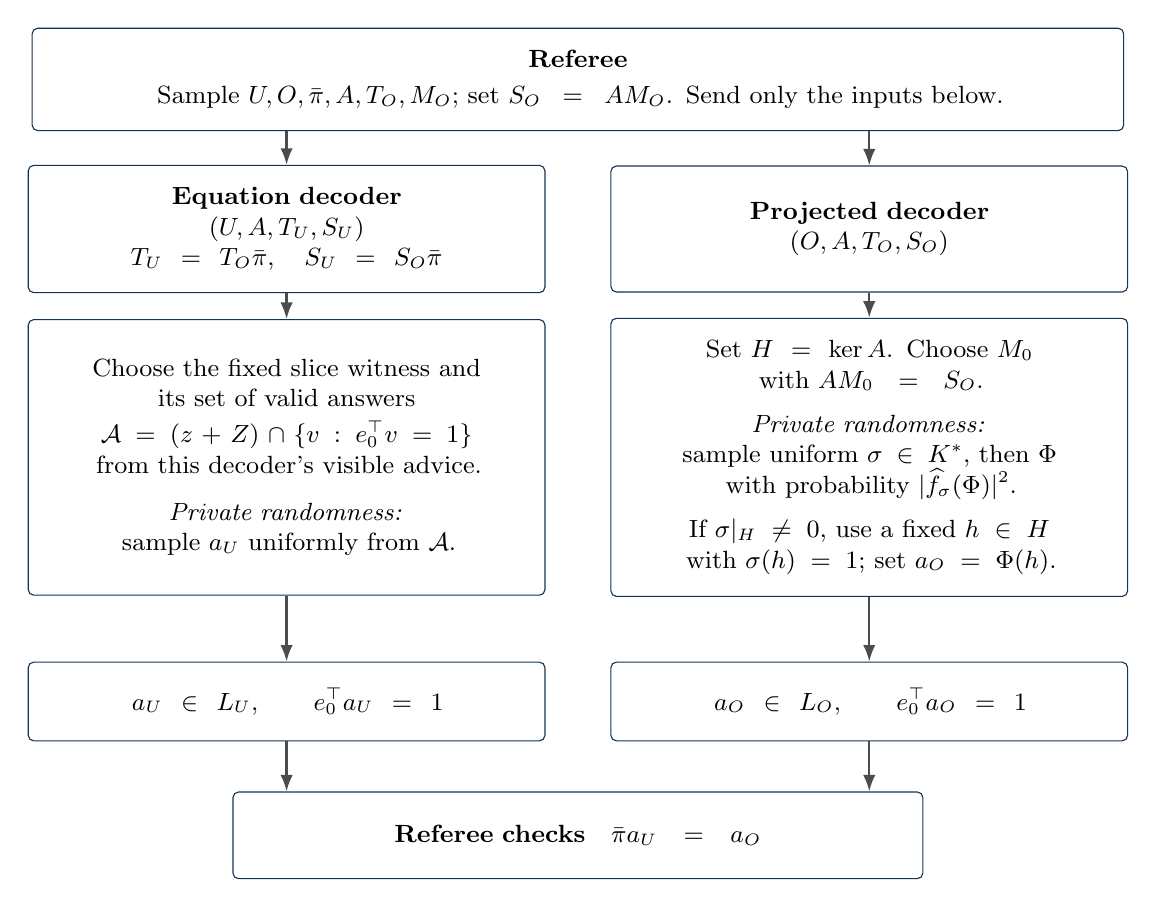
\begin{tikzpicture}[
  x=1cm,y=1cm,
  every node/.style={font=\small},
  box/.style={draw=linkblue!80!black,rounded corners=2pt,
    text width=6.0cm,align=center,inner sep=8pt},
  input/.style={box,minimum height=16mm},
  rule/.style={box,minimum height=35mm},
  output/.style={box,minimum height=10mm},
  flow/.style={-{Latex[length=2.1mm]},thick,draw=black!70}
]
\node[box,text width=13.3cm,minimum height=12mm] (sample) at (3.7,0)
  {\textbf{Referee}\\[2pt]
   Sample $U,O,\bar\pi,A,T_O,M_O$; set $S_O=AM_O$.
   Send only the inputs below.};

\node[input] (uinput) at (0,-1.9)
  {\textbf{Equation decoder}\\
   $(U,A,T_U,S_U)$\\
   $T_U=T_O\bar\pi,\quad S_U=S_O\bar\pi$};
\node[input] (oinput) at (7.4,-1.9)
  {\textbf{Projected decoder}\\
   $(O,A,T_O,S_O)$};
\draw[flow] (sample.south -| uinput.north) -- (uinput.north);
\draw[flow] (sample.south -| oinput.north) -- (oinput.north);

\node[rule] (urule) at (0,-4.8)
  {Choose the fixed slice witness and\\its set of valid answers\\[2pt]
   $\mathcal A=(z+Z)\cap\{v:e_0^\top v=1\}$\\
   from this decoder's visible advice.\\[6pt]
   \textit{Private randomness:}\\
   sample $a_U$ uniformly from $\mathcal A$.};
\node[rule] (orule) at (7.4,-4.8)
  {Set $H=\ker A$. Choose $M_0$\\with $AM_0=S_O$.\\[5pt]
   \textit{Private randomness:}\\
   sample uniform $\sigma\in K^*$, then $\Phi$\\
   with probability $|\widehat f_\sigma(\Phi)|^2$.\\[5pt]
   If $\sigma|_H\ne0$, use a fixed $h\in H$\\
   with $\sigma(h)=1$; set $a_O=\Phi(h)$.};
\draw[flow] (uinput) -- (urule);
\draw[flow] (oinput) -- (orule);

\node[output] (uoutput) at (0,-7.9)
  {$a_U\in L_U,\qquad e_0^\top a_U=1$};
\node[output] (ooutput) at (7.4,-7.9)
  {$a_O\in L_O,\qquad e_0^\top a_O=1$};
\draw[flow] (urule) -- (uoutput);
\draw[flow] (orule) -- (ooutput);

\node[box,text width=8.2cm,minimum height=11mm] (verify) at (3.7,-9.6)
  {\textbf{Referee checks}\quad $\bar\pi a_U=a_O$};
\draw[flow] (uoutput.south) -- (verify.north -| uoutput.south);
\draw[flow] (ooutput.south) -- (verify.north -| ooutput.south);
\end{tikzpicture}
\caption{The two decoders use independent random tapes. Neither receives the
sampled $M_O$ or the projection $\bar\pi$; the right decoder chooses its own
representative $M_0$ from the visible advice. Every displayed advice map
includes its affine intercept, through the homogeneous coordinate. The
transferred slice is used only to analyze these private rules: the right
decoder does not use the left witness or answer set. If the left advice is
not good, or if $\sigma|_H=0$ on the right, that decoder returns an arbitrary
valid answer.}
\label{fig:advice}
\end{figure}

\FloatBarrier

\begin{lemma}[A transferred slice gives agreement]
\label{lem:fourier-coset-decoding}
Fix joint data satisfying Lemma~\ref{lem:projected-witness}.  Conditional
on these data, the two rules just defined, using independent randomness,
agree under $\bar\pi$ with probability at least
\begin{equation}
 2^{-\ell r_{\rm s}}(\alpha/8)^2\,2^{-r_{\rm s}}.
 \label{eq:conditional-decoding}
\end{equation}
\end{lemma}

\begin{proof}
Put $Z'=\bar\pi Z$, so $\dim Z'\le r_{\rm s}$.  The projected column
specifications in the row fiber fix the restriction $N|_{Z'}$ to a linear
map $b:Z'\to H$.  The resulting affine slice is nonempty; choose one
$N_*$ in it.  For every $\sigma\in K^*$ define
\[
 C_\sigma=\E\bigl[f_\sigma(N)(-1)^{\sigma(Nz')}
                       \mid N|_{Z'}=b\bigr].
\]
The character expansion of Equation~\eqref{eq:transferred-witness} gives
\[
 \E_\sigma\bigl[(-1)^{\sigma(M_0z'+u)}C_\sigma\bigr]
 \ge\alpha/4,
 \qquad\text{so}\qquad
 \E_\sigma|C_\sigma|\ge\alpha/4.
\]
Exactly a fraction $2^{-\dim H}$ of the characters have trivial
restriction to $H$.  Since $\dim H\ge\ell-r_{\rm s}$ and
$|C_\sigma|\le1$, Equation~\eqref{eq:matrix-parameters} implies
\begin{equation}
 \E_\sigma\bigl[\mathbf 1_{\{\sigma|_H\ne0\}}|C_\sigma|\bigr]
 \ge\alpha/8.
 \label{eq:nontrivial-correlation}
\end{equation}

The annihilator in $X^*$ of matrices vanishing on $Z'$ is $H^*\otimes Z'$.
For $\theta_\sigma=(\sigma|_H)\otimes z'$, Fourier expansion on the
affine slice therefore gives
\[
 C_\sigma
 =\sum_{\Phi\in\theta_\sigma+H^*\otimes Z'}
       \widehat f_\sigma(\Phi)
       (-1)^{\langle\Phi+\theta_\sigma,N_*\rangle}.
\]
This sum has $2^{\dim H\dim Z'}\le2^{\ell r_{\rm s}}$ terms.
Cauchy--Schwarz, first on each sum and then in the average over $\sigma$,
shows from Equation~\eqref{eq:nontrivial-correlation} that
\begin{align*}
 &\E_\sigma\left[
   \mathbf 1_{\{\sigma|_H\ne0\}}
   \sum_{\Phi\in\theta_\sigma+H^*\otimes Z'}
             |\widehat f_\sigma(\Phi)|^2\right]\\
 &\hspace{15mm}\ge
 2^{-\ell r_{\rm s}}
 \E_\sigma\bigl[\mathbf 1_{\{\sigma|_H\ne0\}}C_\sigma^2\bigr]
 \ge 2^{-\ell r_{\rm s}}(\alpha/8)^2.
\end{align*}
This is a lower bound on the probability that the $O$-decoder samples a
nontrivial restriction and a frequency in the indicated coset.

Every such frequency has the form
$\Phi=(\sigma|_H)\otimes z'+\Psi$ with $\Psi\in H^*\otimes Z'$.
For the decoder's choice of $h$ it satisfies
\[
 \Phi(h)=z'+\Psi(h)\in z'+Z'.
\]
As already proved, a frequency of positive mass gives first bit one.
Equation~\eqref{eq:projected-answer-set} therefore places the returned
vector in $\bar\pi\mathcal A$.  Independently, the $U$-decoder samples
uniformly from $\mathcal A$ and chooses a preimage with probability at
least $1/|\mathcal A|\ge2^{-r_{\rm s}}$.  Multiplying the bounds proves
Equation~\eqref{eq:conditional-decoding}.
\end{proof}

\begin{proof}[Proof of Proposition~\ref{prop:matrix-decoding}]
Use the two decoders above.  Lemma~\ref{lem:projected-witness} supplies a
set of joint data of probability at least $\gamma_1$, and
Lemma~\ref{lem:fourier-coset-decoding} gives the stated conditional
agreement on that set.  Thus one may take
\[
 \gamma=\gamma_1\,2^{-\ell r_{\rm s}}(\alpha/8)^2\,2^{-r_{\rm s}}>0.
\]
The largeness requirements for $k$ come only from
Theorem~\ref{thm:shortcode}, the concentration bound in
Lemma~\ref{lem:good-row-advice}, and the total variation estimate in
Lemma~\ref{lem:projected-tv}.  They are uniform in the parity instance
and table family.  Witness choices and Fourier sampling need not be efficient:
they define strategies in a finite game for the soundness argument.
Finally, averaging over the provers' independent random tapes also gives
deterministic strategies with at least the same agreement probability.
\end{proof}

\section{Clean coordinates and the soundness gap}
\label{sec:clean}

Proposition~\ref{prop:matrix-decoding} converts high acceptance of the
matrix test into agreement between two local strategies supplied with
correlated linear advice.  We now bound the value of this advice
experiment on a NO parity instance.  The use of vanishing advice is part
of the smooth outer-game framework of
\cite[Sections~3.3--3.4]{KMS17}.  We give the full local reconstruction
argument for the present occurrence-indexed questions.  The key is to
identify singleton coordinates on which both advice slopes vanish.
After fixing the data outside those coordinates, their question pairs
have the ordinary independent equation--variable law.  Each side can
then reconstruct its original advice input from its own remaining
questions and the fixed data.  This defines strategies for an ordinary
parallel repetition, whose value bounds the original agreement.

\subsection{Classical projection-game repetition}

We use the following form of the parallel repetition theorem of
Dinur and Steurer.  The value here is the ordinary classical value:
each prover answers using only its own question.  A projection
constraint maps each answer on one side to its required answer on the
other side.

\begin{theorem}[Projection-game repetition]
\label{thm:repetition}
Let $G$ be a finite bipartite projection game, with an arbitrary
probability distribution on its constraint occurrences.  Question sets
and answer alphabets may be arbitrary finite sets, and parallel
constraint occurrences are allowed.  The game $G^{\otimes n}$ samples
$n$ independent occurrences, sends each prover its tuple of questions,
and accepts if all $n$ projection constraints hold.  For every integer
$n\ge1$ and every $0<g<1$,
\begin{equation}
 \val(G)\le 1-g
 \quad\Longrightarrow\quad
 \val(G^{\otimes n})\le (1-g^2/16)^n.
 \label{eq:projection-repetition}
\end{equation}
The bound is independent of the question-set and alphabet sizes.
\end{theorem}

This is Corollary~1.2 of \cite{DS14}.  Their Section~2.1 permits
nonnegative edge weights and
parallel edges, and Section~2.2 defines the independent product used
here.  Thus the theorem applies to any finite weighted question
distribution in our constructions.  Interchanging the provers, if
necessary, matches the direction of the projection.  Private
randomization and shared randomness independent of the questions do not
increase classical value: sample complete deterministic answer tables
using that randomness before the questions arrive, and average their
success probabilities.

\subsection{Vanishing advice on clean coordinates}

Let $\mathcal E$ be the parity instance from Section~\ref{sec:game},
with three distinct variable IDs in each equation occurrence.  Recall
its ordinary equation--variable game $G_{\mathcal E}$: the first
prover receives an equation and answers with a satisfying triple;
the second receives a uniformly selected variable from that equation
and answers with a bit.  On a NO instance,
Equation~\eqref{eq:base-game-gap} gives
$\val(G_{\mathcal E})\le14/15$.

Recall the advice experiment of Section~\ref{sec:matrix}, taking $k$
along integer cubes larger than one and setting $\beta=k^{-2/3}$.
An ordered tuple $U$ consists of $k$ independent equation samples.
Independently in each block, with probability $\beta$ we keep a uniformly
chosen variable position, and otherwise keep the entire equation.
This produces $O$ and the answer projection $\bar\pi:L_U\to L_O$
of Equation~\eqref{eq:outer-projection}.  Independently choose
\[
 A:K\to\F_2^{r_{\rm s}},\qquad
 T_O:L_O\to W,\qquad M_O:L_O\to K
\]
uniformly, and put $S_O=AM_O$.  The two inputs, respectively, are
\begin{equation}
 (U,A,T_O\bar\pi,S_O\bar\pi)
 \quad\text{and}\quad
 (O,A,T_O,S_O).
 \label{eq:clean-advice-inputs}
\end{equation}
The matrix $M_O$ beyond $S_O$ is not part of either input.  Each prover
must return an actual answer, equivalently a vector whose first
coordinate is one in its respective answer space.

\begin{lemma}[Clean-coordinate bound]
\label{lem:clean}
If $\OPT(\mathcal E)\le 4/5$, every pair of local randomized strategies
in the advice experiment satisfies
\begin{equation}
 \Pr\bigl[\bar\pi(a_U)=a_O\bigr]
 \le \left(1-\frac{\beta\,2^{-\dim W-r_{\rm s}}}{3600}\right)^k
 \le
 \exp\!\left(
 -\frac{2^{-\dim W-r_{\rm s}}}{3600}\,k^{1/3}
 \right).
 \label{eq:clean-agreement-bound}
\end{equation}
In particular, the upper bound tends to zero uniformly over the parity
instance as $k$ tends to infinity along cubes, with the advice spaces
fixed.
\end{lemma}

\begin{proof}
Fix an arbitrary pair of local randomized strategies in the advice
experiment.  We first condition on $A$ and combine the two visible
advice maps into
\[
 D_O=(T_O,S_O):L_O\longrightarrow E_A,
 \qquad E_A=W\oplus\im A.
\]
Conditional on the questions and projection choices, the intercept
$c_O$ and all block slope columns of $D_O$ are independent uniform
elements of $E_A$.  Indeed, the columns of $T_O$ and $M_O$ are
independent and uniform, and applying $A$ to a uniform column gives a
uniform element of $\im A$.  This coefficient law depends only on
whether a block is an equation or a singleton, and not on any equation
ID, variable ID, or selected position.  In particular, $c_O$ is
independent of all block data.

Call coordinate $i$ \emph{clean} if it is projected to a singleton
and its one advice slope $d_i\in E_A$ is zero.  Conditional on $A$,
the clean indicators are independent, with common probability
\begin{equation}
 p_A=\frac{\beta}{\abs{E_A}}
     =\beta\,2^{-\dim W-\rank A}.
 \label{eq:clean-probability}
\end{equation}
More precisely, for every equation occurrence $e$ and position
$j\in[3]$,
\begin{equation}
 \Pr[e_i=e,\ i\text{ is a clean singleton at position }j\mid A]
 =\omega_e\,\frac{\beta}{3\abs{E_A}}.
 \label{eq:clean-joint-law}
\end{equation}
Thus, conditional on being clean, a coordinate has precisely the
ordinary equation--variable distribution.

Let $I\subseteq[k]$ be the clean set.  For the analysis, let $R$ consist
of $A$, $I$, the original intercept $c_O$, and the following data for
every $i\notin I$: its equation occurrence, whether the block was
retained or projected, the selected position in the latter case, and
its advice slope columns.  No witness, decoder output, agreement event,
or response randomness is included in $R$.

For each value $R=r$ of positive probability, regard the clean set
$I$ recorded in $r$ as fixed.  When $I$ is nonempty, we will use $r$
as constant data when defining two strategies for
$G_{\mathcal E}^{\otimes\abs{I}}$.
Each strategy will reconstruct one original advice input from its own
product-game questions, apply the corresponding original response rule,
and retain the answers in the clean slots.

Conditional on $R=r$, the pairs
\[
 (e_i,v_{e_i,j_i}),\qquad i\in I,
\]
are independent question pairs of $G_{\mathcal E}$.  Indeed, conditional
on $A$, the coordinate data are independent, and
Equation~\eqref{eq:clean-joint-law} shows that conditioning on the clean
mask preserves the ordinary law in each clean coordinate.  The outside
coordinate data and the independent intercept impose no further
condition on these pairs.

We now verify the two reconstructions, including the affine intercept
shared across the blocks.  An equation with right-hand side $b_e$ has actual
bits $x,y,b_e t_0+x+y$.  Pulling back a singleton slope $d_i$ thus
produces the two slopes
\begin{equation}
 (d_i,0),\quad (0,d_i),\quad (d_i,d_i)
 \label{eq:clean-padded-slopes}
\end{equation}
at positions one, two, and three, respectively.  The intercept of
$D_U=D_O\bar\pi$ is
\begin{equation}
 c_U=c_O+
 \sum_{\substack{i\text{ projected to a singleton}\\j_i=3}}
 b_{e_i}d_i.
 \label{eq:clean-intercept}
\end{equation}
For a clean coordinate, every slope in
Equation~\eqref{eq:clean-padded-slopes} is zero and its contribution to
Equation~\eqref{eq:clean-intercept} is zero.  All remaining terms in
that equation are determined by $r$.

The equation side receives its occurrences $e_i$ for $i\in I$.
Together with $r$, they specify all of $U$.  Its two advice slopes in
each clean block are zero, while $r$ determines every other slope and
the full intercept.  These coefficients reconstruct both padded advice
maps without using any clean selected position or variable question.
The variable side receives the variable question for each $i\in I$.
Together with $r$, these specify all of $O$.  Its clean singleton
slopes are zero, and $r$ supplies every other slope and the original
intercept.  These coefficients reconstruct its two advice maps without
using any clean equation.  Repeated IDs across different blocks cause no
additional restriction: questions were sampled independently with
replacement, and answers use the local copies specified in
Section~\ref{sec:game}.

These reconstructions define the promised product-game strategies:
each side applies its original response rule to the reconstructed
input and retains its answers in the slots $I$, in their original
order.  Their equation answers are satisfying triples because the
original answers are valid.  For every realization of the clean
questions and response randomness, full agreement in the advice
experiment implies acceptance in every clean slot.  If $I=\varnothing$,
the conditional success probability is at most one.  Otherwise,
\[
 \Pr[\bar\pi a_U=a_O\mid R=r]
 \le \val(G_{\mathcal E}^{\otimes\abs{I}})
 \le \left(1-\frac{1}{3600}\right)^{\abs{I}}.
\]
The first inequality uses the strategies just constructed and the
conditional product law.  The second uses
Theorem~\ref{thm:repetition} and Equation~\eqref{eq:base-game-gap}.
The original response rules are evaluated only at their original
local inputs; $r$ indexes the auxiliary product-game strategies.
Thus the final bound holds for every $r$, including $I=\varnothing$
when its right-hand side is interpreted as one.

Finally, conditional on $A$, the size of $I$ has distribution
$\operatorname{Binomial}(k,p_A)$.  Averaging the preceding inequality
first over $R$ conditional on $A$, and then over $A$, gives
\begin{align*}
 \Pr\bigl[\bar\pi(a_U)=a_O\bigr]
 &\le \E_A\left(1-\frac{p_A}{3600}\right)^k\\
 &\le\left(1-\frac{\beta\,2^{-\dim W-r_{\rm s}}}{3600}\right)^k\\
 &\le \exp\!\left(
 -\frac{k\beta\,2^{-\dim W-r_{\rm s}}}{3600}
 \right),
\end{align*}
since $\rank A\le r_{\rm s}$.  Substituting
$k\beta=k^{1/3}$ proves Equation~\eqref{eq:clean-agreement-bound}.
\end{proof}

\subsection{The matrix-game gap}

We can now compare the upper bound for every advice strategy with the
strategies extracted from a highly accepting matrix labeling.

\begin{proposition}[A fixed gap with adjustable completeness]
\label{prop:matrix-gap}
Fix $p_*>0$ and choose the latent and shortcode data in the order of
Equation~\eqref{eq:matrix-parameters}.  For every sufficiently large
cube $k$, the matrix game $\mathcal G$ constructed from a weighted
parity instance $\mathcal E$ with distinct positions satisfies
\[
 \begin{aligned}
 \OPT(\mathcal E)\ge1-\xi
 &\quad\Longrightarrow\quad
 \val(\mathcal G)\ge1-k\xi-p_*/2,\\
 \OPT(\mathcal E)\le4/5
 &\quad\Longrightarrow\quad
 \val(\mathcal G)\le99/100.
 \end{aligned}
\]
The lower threshold on $k$ depends only on the fixed latent and
shortcode data, not on $\mathcal E$ or $\xi$.
\end{proposition}

\begin{proof}
Completeness is Lemma~\ref{lem:outer-completeness}.  For soundness,
fix a labeling of $\mathcal G$.  Its restored table functions satisfy
the folding and sharing identities of Section~\ref{sec:game}.
Proposition~\ref{prop:matrix-decoding} supplies a constant $\gamma>0$
and, for every sufficiently large cube $k$, gives local advice
strategies with agreement at least $\gamma$ whenever those functions
have matrix-test acceptance at least $0.99$.  For all sufficiently large
cubes $k$, the upper
bound in Equation~\eqref{eq:clean-agreement-bound} is smaller than
$\gamma$.
Lemma~\ref{lem:clean} contradicts the existence of those strategies
whenever $\OPT(\mathcal E)\le4/5$.  All thresholds are uniform over
the parity instance.
\end{proof}

The order matters: $p_*$ can be made arbitrarily small before the
gadget parameters are fixed, and $\xi$ can be made arbitrarily small
after $k$ is fixed.  Thus the same NO gap is compatible with any
prescribed small completeness error.

\section{Completion of the reduction}
\label{sec:finish}

The matrix game has a fixed soundness gap and an arbitrarily small
completeness error.  We now obtain the form required by
Theorem~\ref{thm:ugc}: unweighted, simple bipartite games with arbitrary
prescribed errors.  Rounding the occurrence weights and subdividing
each occurrence will preserve a fixed gap.  One application of
alphabet-independent repetition then completes the proof.

\subsection{Removing weights and repeated edges}

We use the following elementary construction for weighted permutation
constraints.  At this intermediate stage, a constraint occurrence may
be a loop, and several occurrences may join the same vertices.

\begin{lemma}[Rounding and subdivision]
\label{lem:unweighted-subdivision}
Let $H$ be a finite permutation-constraint game with $h\ge1$ positive
rational occurrence weights summing to one.  For every positive
rational $\tau$, put $Q=\lceil h/\tau\rceil$.  There is a
deterministic construction of an unweighted simple bipartite game $B$
with $4Q$ edges and the same alphabet such that
\begin{equation}
 \left|\val(B)-\left(1-\frac{1-\val(H)}4\right)\right|
 \le\frac{\tau}{4}.
 \label{eq:rounded-subdivision-value}
\end{equation}
If the constraints of $H$ are translations on a finite binary vector
space, so are those of $B$.  For fixed $\tau$, when $H$ is listed by its
vertices, occurrences, permutation tables, and binary rational weights,
the construction takes polynomial time in its encoding length.
\end{lemma}

\begin{proof}
Write the occurrence weights as $w_1,\ldots,w_h$.  Start with
$n_e=\lfloor Qw_e\rfloor$, and add one to the
$Q-\sum_e\lfloor Qw_e\rfloor$ entries having largest fractional parts,
breaking ties in a fixed order.  Then
\[
 n_e\ge0,\qquad \sum_e n_e=Q,\qquad
 |w_e-n_e/Q|\le1/Q.
\]
The weight differences sum to zero.  Consequently, for every labeling,
the change in the weight of its satisfied-occurrence set is at most
\[
 \frac12\sum_{e=1}^h|w_e-n_e/Q|
 \le\frac{h}{2Q}\le\tau.
\]
Replace each occurrence $e$ by $n_e$ copies, omitting it if $n_e=0$.
The resulting unweighted multigraph $H'$ has $Q$ occurrences and
$|\val(H')-\val(H)|\le\tau$.

Orient each occurrence $e$ of $H'$ from $u$ to $v$, writing its
constraint as $a_v=\rho_e(a_u)$.  Replace it by the path
\[
 u\;--\;p_e\;--\;q_e\;--\;r_e\;--\;v,
\]
using three fresh interior vertices for \emph{every occurrence}.
Place all original vertices and all $q_e$ on the left, and all
$p_e,r_e$ on the right.  In the direction from $u$ to $v$, put identity
permutations on the first three edges and $\rho_e$ on the last.
When expressing an edge in left-to-right orientation, invert its
permutation if needed.  Give all $4Q$ edges equal weight.

Fix labels at the original vertices.  A satisfied occurrence extends
to four satisfied edges.  A violated occurrence cannot extend to four,
but propagating labels along the first three edges satisfies exactly
three.  Since the interiors are disjoint, these extensions can be
chosen independently.  Maximizing over the original labels gives the
exact identity
\begin{equation}
 \val(B)=1-\frac{1-\val(H')}{4}.
 \label{eq:bipartization-value}
\end{equation}
This proves Equation~\eqref{eq:rounded-subdivision-value}.

A loop becomes a four-cycle with three distinct new vertices.
Parallel occurrences have disjoint interiors.  Thus each left--right
vertex pair carries at most one edge, so $B$ is simple.  An inverse
binary translation is the same translation, and an identity is
translation by zero; the claimed constraint form is preserved.

Finally, $Q\le h/\tau+1$ is polynomially bounded for fixed $\tau$.
Integer division and exact comparison of rational remainders compute
the $n_e$ in polynomial time and bit complexity.  Listing their $Q$
copies and the $3Q$ new vertices is therefore polynomial as well.
\end{proof}

\subsection{The final reduction}

\begin{proof}[Proof of Theorem~\ref{thm:ugc}]
Fix $\eps,\delta\in(0,1/2)$.  Choose positive rational
$\eps_0\le\eps$ and $\delta_0\le\delta$.  We will take
$\tau\le1/200$ when applying the rounding and subdivision lemma.
For any matrix game $H$ satisfying the NO bound
$\val(H)\le99/100$, the resulting game $B$ then satisfies
\begin{equation}
 \val(B)\le1-\frac{1/100-\tau}{4}\le1-\frac1{800}.
 \label{eq:post-subdivision-gap}
\end{equation}
This gap does not depend on the alphabet.  We can therefore use
alphabet-independent repetition to choose its exponent before the
latent construction fixes that alphabet.  Choose an integer $t\ge1$
such that
\begin{equation}
 \left(1-\frac1{10240000}\right)^t\le\delta_0.
 \label{eq:final-repetition-gap}
\end{equation}
For example, $t\ge\lceil10240000\log(1/\delta_0)\rceil$ suffices.
By Theorem~\ref{thm:repetition}, this exponent reduces every projection
game of value at most $1-1/800$ to value at most $\delta_0$.

Choose positive rational parameters
\begin{equation}
 p_*\le\frac{\eps_0}{t},\qquad
 \tau\le\min\left\{\frac1{200},\frac{\eps_0}{t}\right\}.
 \label{eq:final-errors}
\end{equation}
Choose the latent rank threshold $r_*$ from Lemma~\ref{lem:latent},
put $\eta=2^{-r_*}/16$, and choose the corresponding shortcode
parameters $\alpha,r_{\rm s}$, using a positive rational lower bound
for $\alpha$.  Then choose a sufficiently large $\ell$, as specified
in Equation~\eqref{eq:matrix-parameters}, and fix the corresponding
latent data $(\mathcal V,K,C,\mu)$ and a splitting
$\mathcal V=K\oplus W$, with $K=\F_2^\ell$.

Once the rational budgets are fixed, these choices are effective.
For rational $p_*$, the effective assertion of Lemma~\ref{lem:latent}
supplies all the finite latent data, including a computable rational
noise law, by a terminating deterministic construction.  The effective bounds stated after
Theorem~\ref{thm:shortcode} supply the rational choice of $\alpha$ and
the dimension thresholds, including $m_0(\eta,\ell)$ after $\ell$ has
been fixed.

Next choose a cube $k\ge8$ large enough for
Proposition~\ref{prop:matrix-gap}.
Such a cube can be found by checking the estimates used in its proof.
Write $m=1+2k$ and $\beta=k^{-2/3}$; since $k$ is a cube, $\beta$ is
rational.  Require $m\ge m_0(\eta,\ell)$ and
\[
 \frac{\alpha^2}{32}\,2^{(\ell-r_{\rm s})(m-r_{\rm s})}
 >(2r_{\rm s}+1)(\ell+m).
\]
The latter is a sufficient rational condition for the union bound in
Lemma~\ref{lem:good-row-advice} to be less than one.  For witness
transfer in Lemma~\ref{lem:projected-witness}, require
\[
 \frac14\left[
 \left(1+\frac{|\mathcal V|-1}{3}\beta^2\right)^k-1\right]
 <\frac{\gamma_1^2}{(1+\alpha/4)^2},
\]
where $\gamma_1$ is from
Equation~\eqref{eq:projected-witness-mass}.  The left-hand side is the
square of the total-variation bound.  For the final contradiction,
require
\[
 \left(1-\frac{\beta\,2^{-\dim W-r_{\rm s}}}{3600}\right)^k
 <\gamma,
\]
with $\gamma$ from Proposition~\ref{prop:matrix-decoding}.  All these
conditions are rational and hold for sufficiently large cubes $k$.
Enumerating cubes until they hold therefore finds a suitable $k$;
the search cost depends only on the two prescribed errors and is
incurred before the input formula is used.

Finally, with $k$ fixed, choose a positive rational
\begin{equation}
 \xi<\min\left\{\frac1{100},\frac{\eps_0}{2kt}\right\}.
 \label{eq:final-parity-error}
\end{equation}
Every choice depends only on the two prescribed errors.  In
particular, $r_*$ is fixed before $\ell$, the advice dimensions before
$k$, and $k$ before the parity error $\xi$.

Given a 3SAT formula, apply Theorem~\ref{thm:parity} and
Lemma~\ref{lem:distinct-parity}, and construct the matrix game $H$
of Section~\ref{sec:game}.  Proposition~\ref{prop:matrix-gap} gives
\[
 \begin{array}{ll}
 \text{YES:}&\val(H)\ge1-d,
       \quad d=k\xi+p_*/2\le\eps_0/t,\\[2pt]
 \text{NO:}&\val(H)\le99/100.
 \end{array}
\]
Apply Lemma~\ref{lem:unweighted-subdivision} with $\tau$ to obtain
the unweighted simple bipartite game $B$.  It satisfies
\[
 \begin{array}{ll}
 \text{YES:}&\val(B)\ge1-(d+\tau)/4,\\[2pt]
 \text{NO:}&\val(B)\le1-1/800,
 \end{array}
\]
where the NO bound is Equation~\eqref{eq:post-subdivision-gap}.
The final output is $G=B^{\otimes t}$.  Its NO value is at most
$\delta_0\le\delta$, by Equations~\eqref{eq:projection-repetition}
and \eqref{eq:final-repetition-gap}.  On a YES input, use a labeling
of $B$ coordinatewise.  A union bound gives
\[
 \val(G)\ge1-\frac{t(d+\tau)}4
 \ge1-\eps_0/2\ge1-\eps.
\]

The output has the claimed graph and constraint form.  Its two vertex
sets are the $t$-fold products of the two sides of $B$.  A pair of
product vertices determines at most one edge in each coordinate,
since $B$ is simple, and hence at most one product edge.  Independent
uniform edge sampling is uniform on these product edges.  The
constraints of $H$ are translations on $K$, by
Section~\ref{sec:game}; rounding and subdivision preserve them.
The product of translations with offsets $c_1,\ldots,c_t$ is
translation by $(c_1,\ldots,c_t)$ on $K^t=\F_2^{\ell t}$.  This is
the alphabet $\F_2^s$ in the theorem, with $s=\ell t\ge1$ fixed by
the prescribed errors.

\paragraph{Polynomial encoding.}
Suppose the preprocessed parity instance has $N_{\mathcal E}$ positive
equation occurrences.  There are $N_{\mathcal E}^k$ equation tuples.
The number of tables, noise outcomes, and perturbation vectors for each
tuple is fixed after the parameter choices above, so the number $h$ of
listed matrix-test occurrences is a fixed constant times
$N_{\mathcal E}^k$.  Omit
zero-probability outcomes and retain repeated occurrences separately.
Each weight is a product of $k$ parity weights, a fixed rational
noise probability, and fixed uniform-sampling factors.  It has
polynomial binary length.

Exact table keys and folded representatives are computed by linear
algebra in fixed dimensions, keeping the original variable and
occurrence IDs.  At most $2h$ endpoints appear.  Even comparing every
pair of keys to identify equal vertices takes polynomial time; number
the resulting distinct vertices consecutively.
Largest-remainder rounding uses $Q=\lceil h/\tau\rceil=O(h)$ copies;
subdivision creates $3Q$ new vertices and $4Q$ edges.  The final
product has $(4Q)^t$ edges and polynomially many vertices, because
$t$ is fixed.  Full permutation tables on the fixed alphabet
$\F_2^{\ell t}$ have constant size, and endpoint indices have
$O(t\log(h+1))$ bits.  These observations give a deterministic
polynomial-time explicit construction throughout and complete the
proof.
\end{proof}

\section{Approximation consequences}\label{sec:consequences}

Theorem~\ref{thm:ugc} turns established conditional hardness results
into NP-hardness results. The underlying conditional reductions and
approximation thresholds are due to the cited authors. We give the
additional arguments needed for the exact instance models stated below.
We also record two results from companion
manuscripts. For a maximization problem, ratio
\(r\) means returning value at least \(r\) times the optimum; for a
minimization problem, factor \(c\) means returning value at most \(c\)
times the optimum.
All factors and tolerances below are fixed independently of input size.
In each reduction using Theorem~\ref{thm:ugc}, they determine the
Unique Games errors before its alphabet is chosen. If
\(\mathrm P\ne\mathrm{NP}\), the resulting hardness statements exclude
deterministic polynomial-time approximations at the indicated strict
thresholds.

\subsection{Constraint satisfaction and Vertex Cover}

For \textsc{Max-Cut}, which maximizes the number of edges crossing a
bipartition, Khot, Kindler, Mossel, and O'Donnell's reduction gives
NP-hardness of approximation at every fixed ratio in
\((\alpha_{\mathrm{GW}},1)\), where the Goemans--Williamson constant is
\(\alpha_{\mathrm{GW}}\simeq0.87856\)~\cite[Theorem~1]{KKMO07}.
This matches the semidefinite approximation threshold of Goemans and
Williamson~\cite{GW95}. The reduction uses the Majority Is Stablest
theorem of Mossel, O'Donnell, and Oleszkiewicz~\cite{MOO10}.
For \textsc{Vertex Cover}, which minimizes the number of vertices
meeting every edge, Khot and Regev's reduction gives NP-hardness at
every fixed factor in \((1,2)\)~\cite{KhotRegev2008}.

A constraint satisfaction problem (CSP) is specified here by a finite
nonempty domain \(D\) and a finite family \(\Lambda\) of Boolean
predicates on \(D\), of bounded arity. A weighted \(\Lambda\)-instance
has a finite variable set and a finite collection of predicates from
\(\Lambda\) applied to tuples of variables, with nonnegative rational
weights summing to one. An assignment maps the variables to \(D\);
its value is the total satisfied weight, and \(\operatorname{OPT}\)
is the maximum of this value over all assignments.
Raghavendra's theorem characterizes the optimal approximation
for every fixed language of this form, up to arbitrarily small positive
error, by a basic semidefinite relaxation
\cite[Theorem~1.1 and Corollary~1.3]{Raghavendra08}.
The Vertex Cover result uses its own reduction. Write
\(\operatorname{SDP}_{R}\) for the value of Raghavendra's relaxation,
as defined in~\cite[Section~4.5]{RaghavendraThesis09}.

The fixed-instance form of Raghavendra's theorem and the ordering
theorem below use a strengthened bipartite formulation of Unique Games.
In its YES case, one labeling satisfies every edge incident to at least
a \(1-\zeta\) fraction of left vertices; in its NO case, every labeling
satisfies at most a \(\nu\) fraction of edges. These are uniform
fractions of the left vertices and edges, respectively.
Lemma~\ref{lem:simple-strong-left} gives this promise on an explicit
nonempty simple graph whose common positive left degree can meet any
fixed lower bound and be divisible by any fixed positive integer. It follows
Khot and Regev's normalization and sequence construction
\cite[Lemmas~3.3, 3.4, and~3.6]{KhotRegev2008}, with an additional
restriction that makes the graph simple. Its error parameters and
degree are fixed before the alphabet is chosen, so
Theorem~\ref{thm:ugc} supplies the required premise.

\begin{corollary}[Raghavendra's consequence]\label{cor:raghavendra-consequence}
Let \(J\) be a fixed \(\Lambda\)-instance with
\(A=\operatorname{OPT}(J)<B=\operatorname{SDP}_{R}(J)\).
For every fixed \(0<\eta<(B-A)/2\), it is NP-hard to distinguish
\(\Lambda\)-instances \(I\) satisfying
\[
 \operatorname{OPT}(I)\ge B-\eta
 \qquad\text{from those satisfying}\qquad
 \operatorname{OPT}(I)\le A+\eta.
\]
\end{corollary}
\begin{proof}
For the thesis's common-arity convention
\cite[Definitions~7.2.1--7.2.2]{RaghavendraThesis09}, identify \(D\)
with a fixed \([q]\), and pad every predicate with ignored trailing
arguments to a common positive arity, filling the added positions with
a fixed variable of \(J\), which exists because \(A<B\). This leaves
each applied payoff and its dependence set unchanged, hence preserves
\(\operatorname{OPT}\) and the relaxation of
\cite[Section~4.5]{RaghavendraThesis09}.
In that relaxation, each local distribution is over assignments to
the variables on which its applied payoff actually depends.
When emitting an occurrence, discard only the added trailing positions,
retaining the original predicate from \(\Lambda\) and its weight.

Apply Raghavendra's fixed-instance theorem
\cite[Theorem~7.9]{RaghavendraThesis09} with tolerance \(\eta/2\);
see also \cite[Theorem~1.1 and Lemma~2.3]{Raghavendra08}.
The fixed witness and tolerance determine its strengthened Unique Games
errors, so the formulation above and Theorem~\ref{thm:ugc} supply its
premise, with a fixed alphabet \([M]\). Its verifier instances have
optimum greater than \(B-\eta/2\) in the YES case and at most
\(A+\eta/2\) in the NO case.

We pass from the verifier's probability weights to the stated rational
weights. For this fixed invocation, the construction in
\cite[Sections~7.3.1 and~7.5]{RaghavendraThesis09} gives a local
probability law \(\theta\) on a finite set \(\mathcal S\), after the
alphabet \([M]\) is fixed. A record \(s\in\mathcal S\) specifies an
applied predicate of \(J\), its \(a(s)\) ordered oracle-query strings
in \(D^M\), and the positions filled by their replies. This law may
depend on \(J,\eta,M\), but no varying input parameter enters it.
Rational probability vectors are dense in this finite simplex, so fix
\(\widehat\theta\in\mathbb Q_{\ge0}^{\mathcal S}\) with
\[
 \sum_{s\in\mathcal S}\widehat\theta(s)=1,
 \qquad
 \delta:=\frac12\sum_{s\in\mathcal S}
       |\widehat\theta(s)-\theta(s)|<\frac{\eta}{2}.
\]
This rational table is fixed finite data of the reduction; its
description length may depend on \(J,\eta,M\).

Let \(L_\Phi\) and \(V_\Phi\) be the left and right sides of the
nonempty simple game supplied above, and let \(h\ge1\) be its common
left degree.
List the variables \(V_\Phi\times D^M\) used in Section~7.5 of the
cited thesis. Its outer verifier chooses a uniform left vertex \(u\)
and, independently for each
oracle query, chooses a uniform neighbor of \(u\) and relabels the
query string by that edge's permutation. For each \(s\in\mathcal S\),
\(u\in L_\Phi\), and ordered neighbor tuple in \(N(u)^{a(s)}\), emit
the \(\Lambda\)-predicate prescribed by \(s\) on the resulting query
variables. Fill all positions of any syntactic variable omitted from
the test with the first listed output variable; the applied predicate
is independent of such variables, so this leaves its value unchanged.
Give the occurrence
weight
\[
 \frac{\widehat\theta(s)}{|L_\Phi|h^{a(s)}}.
\]
These weights are nonnegative rationals summing to one. Keeping equal
occurrences separate gives
\(|L_\Phi|\sum_{s\in\mathcal S}h^{a(s)}\) occurrences and
\(|V_\Phi||D|^M\) variables. The local set and every \(a(s)\) are
fixed, while the graph has polynomial size; hence this is a polynomial
occurrence list. The explicit neighbor lists and edge permutations let
us write it in polynomial time. Each weight has polynomial binary
length: it can be represented with a fixed denominator multiplied by
\(|L_\Phi|h^{a(s)}\).

For an assignment \(\sigma\), let \(g_\sigma(s)\in[0,1]\) be its
conditional acceptance probability over these outer choices. The
original and rationalized instances use the same variable set, and
\[
 \bigl|\operatorname{val}_{\widehat\theta}(\sigma)
       -\operatorname{val}_{\theta}(\sigma)\bigr|
 =\left|\sum_{s\in\mathcal S}
       \bigl(\widehat\theta(s)-\theta(s)\bigr)g_\sigma(s)\right|
 \le\delta<\frac{\eta}{2}.
\]
Taking maxima gives the same bound for their optima. The imported gap
therefore yields optimum at least \(B-\eta\) in the YES case and at most
\(A+\eta\) in the NO case, as required.
\end{proof}

\subsection{Ordering constraints}

An ordering CSP uses a global order of the input variables, rather than
an assignment from a fixed finite domain. Fix an integer \(k\ge2\) and
a nonempty proper subset \(\Pi\subset S_k\), where \(S_k\) is the set
of permutations of \(\{1,\ldots,k\}\). In the finite
probability-weighted model of Guruswami, H\aa stad, Manokaran,
Raghavendra, and Charikar~\cite[Definition~8.2]{GuruswamiEtAl2011OrderingCSP},
we use an explicitly listed finite variable set \(V\) and a finite list of
constraint occurrences. Their nonnegative rational weights are encoded
by binary numerators and denominators and sum to one. Every occurrence is an
ordered \(k\)-tuple \((v_1,\ldots,v_k)\) of distinct variables,
satisfied by a linear order \(\prec\) when
\[
 v_{\pi(1)}\prec\cdots\prec v_{\pi(k)}
 \quad\text{for some }\pi\in\Pi.
\]
Write \(\OPT_\Pi(I)\) for the maximum satisfied weight. A uniform
random order satisfies expected weight \(\rho_\Pi=|\Pi|/k!\).
Since \(\OPT_\Pi(I)\le1\), it is a \(\rho_\Pi\)-approximation.
For fixed \(k\), conditional expectation derandomizes this guarantee.
After any prefix of the order has been exposed, a constraint has at
most \(k!\) possible relative orders consistent with that prefix.
Its conditional success probability is therefore computable exactly;
choosing each next variable to preserve the expected value takes a
polynomial number of exact rational operations of polynomial bit length.
The size of \(V\) is part
of the input, so this is not a CSP over the fixed finite domain used
in the preceding corollary.

\begin{corollary}[Ordering-CSP consequence]\label{cor:ordering-csp}
Fix \(k\ge2\) and \(\varnothing\ne\Pi\subsetneq S_k\), and put
\(\rho_\Pi=|\Pi|/k!\). For every fixed
\(0<\varepsilon<(1-\rho_\Pi)/2\), it is NP-hard to distinguish finite
weighted \(\Pi\)-ordering-CSP instances \(I\) satisfying
\[
 \OPT_\Pi(I)\ge1-\varepsilon
 \qquad\text{from those satisfying}\qquad
 \OPT_\Pi(I)\le\rho_\Pi+\varepsilon.
\]
Consequently, approximation at every fixed ratio
\(r\in(\rho_\Pi,1]\) is NP-hard. Together with the random-ordering
guarantee, this gives the optimal threshold \(\rho_\Pi\).
\end{corollary}
\begin{proof}
Proposition~\ref{prop:finite-ordering-transfer} constructs the stated
finite instance from a simple strong-left Unique Games instance. It
uses the local gap and analytic estimates of
Guruswami et al.~\cite{GuruswamiEtAl2011OrderingCSP} and fixes the
required game errors and degree conditions before the alphabet is
chosen. Lemma~\ref{lem:simple-strong-left} supplies that game from
Theorem~\ref{thm:ugc}; composing the reductions proves the displayed
gap for the original predicate \(\Pi\).

For a fixed \(r\in(\rho_\Pi,1]\), choose the positive error still
smaller so that \(\varepsilon<(r-\rho_\Pi)/(1+r)\). Then
\(r(1-\varepsilon)>\rho_\Pi+\varepsilon\), so an
\(r\)-approximation would distinguish the two cases.
\end{proof}

For \textsc{Maximum Acyclic Subgraph} in the finite weighted
directed-graph model, take \(k=2\) and \(\Pi=\{12\}\) in one-line
notation. A constraint \((u,v)\) asks that the edge point forward;
forward edges form an acyclic subgraph, and every acyclic subgraph has
a topological order. Its threshold is therefore \(1/2\).
For \textsc{Betweenness}, the constraint \((a,b,c)\) asks that \(b\)
lie between \(a\) and \(c\), so \(\Pi=\{123,321\}\subset S_3\) and
the threshold is \(2/3!=1/3\)
\cite[Theorem~1.1 and Section~1.2]{GuruswamiEtAl2011OrderingCSP}.
These finite weighted consequences have near-perfect completeness
with fixed positive error.

\subsection{Cut, deletion, and clustering consequences}

For the cut problems of Chawla, Krauthgamer, Kumar, Rabani, and
Sivakumar~\cite[Section~1]{CKKRS2006}, let \(G=(V,E)\) be a finite
undirected graph with positive rational edge costs \(c_e\), and let
\(\mathcal D=\{\{s_i,t_i\}:1\le i\le k\}\) contain \(k\ge1\)
distinct demand pairs with \(s_i\ne t_i\). For \(M\subseteq E\), write
\(c(M)=\sum_{e\in M}c_e\), and let \(q_{\mathcal D}(M)\) count
the demand pairs disconnected in \(G-M\).
Weighted \textsc{Multicut} minimizes \(c(M)\) subject to
\(q_{\mathcal D}(M)=k\). Their nonuniform \textsc{Sparsest Cut}
search problem minimizes \(c(M)/q_{\mathcal D}(M)\) over cutsets
\(M\) with \(q_{\mathcal D}(M)>0\). Only the selected pairs carry
unit demand; they need not be all vertex pairs.

For weighted Min-\(2\mathrm{CNF}^{\equiv}\) Deletion, the input
consists of clauses \((\ell\equiv\ell')\) with positive rational
weights, where \(\ell,\ell'\) are Boolean literals, and an assignment
pays the total weight of false clauses. The allowed clauses therefore
express equality or disequality of variables.

In the arbitrary weighted-graph form of \textsc{Correlation Clustering},
each present edge has a \(+\) or \(-\) label and a nonnegative rational
weight. A partition into any number of clusters pays for \(+\) edges
whose endpoints lie in different clusters and \(-\) edges whose
endpoints lie in the same cluster. Missing edges carry no penalty.
This is the minimum-disagreements objective of
\cite[Section~2.1]{DemaineEtAl2006Clustering}.

\begin{corollary}[Cut, deletion, and clustering hardness]
\label{cor:cut-clustering}
For every fixed real constant \(C>1\), it is NP-hard to approximate
each of the four minimization problems above within factor \(C\).
For \textsc{Sparsest Cut}, this is hardness of the search task under
polynomial-time Cook reductions: the algorithm must output a cutset,
not only an estimate of the optimum. Consequently, unless
\(\mathrm P=\mathrm{NP}\), none of these problems admits a deterministic
polynomial-time approximation with any fixed constant factor.
\end{corollary}
\begin{proof}
Corollary~1.3 of \cite{CKKRS2006} gives the first three conclusions
under its ordinary edge-value Unique Games hypothesis.
For a requested factor \(C\), use its hardness statement at any fixed
larger factor \(L\): a \(C\)-approximation would also be an
\(L\)-approximation.
To supply that hypothesis, orient the bipartite constraints of
Theorem~\ref{thm:ugc} left-to-right, renumber its fixed alphabet as
\([d]\) with \(d=2^s\ge2\), and give its edges equal weights summing
to one. Padding the smaller vertex side with isolated questions if
needed preserves both value and polynomial size. The search-version
qualification for \textsc{Sparsest Cut} is in Section~1.3 of the
cited source.

For \textsc{Correlation Clustering}, the hard \textsc{Multicut}
instances in~\cite[Section~2.1]{CKKRS2006} have distinct antipodal
demand pairs inside \(d\)-cubes, while the edges of the Multicut graph
are cube edges or join different cubes. Here \(d\ge2\), unchanged by
Lemma~1.5 of
that source, so the demand pairs are nonedges. The transformation of
Demaine, Emanuel, Fiat, and Immorlica
\cite[Theorem~4.7 and Corollary~4.8]{DemaineEtAl2006Clustering}
therefore creates no opposite-signed parallel edges. It preserves the
optimum and converts every clustering into a multicut of no greater
cost, so the same fixed-factor hardness transfers.
\end{proof}

The separate manuscript
\cite[Theorem~1.1]{OpenAIUniformSparsest2026} proves
NP-hardness at every fixed factor \(C>1\) for the bipartition objective with
nonnegative rational capacities and exactly unit demand between every
pair of distinct vertices. This uniform-demand theorem does not depend on
Theorem~\ref{thm:ugc} and is not supplied by the nonuniform reduction
above.

\paragraph{Kernel clustering.}
A separate companion application concerns the following maximization
problem. For \emph{identity-target kernel clustering}, fix an integer \(k\ge3\).
An input is an explicitly represented rational symmetric matrix
\(A=(a_{pq})_{p,q=1}^N\succeq0\) with \(A\mathbf1=0\), where
\(\mathbf1\) is the all-ones vector.
An assignment \(\sigma:\{1,\ldots,N\}\to\{1,\ldots,k\}\) has value
\[
 \val_A(\sigma)=\sum_{p,q=1}^N
 a_{pq}\mathbf1_{\{\sigma(p)=\sigma(q)\}},
 \qquad
 \OPT_k(A)=\max_\sigma\val_A(\sigma).
\]
The sum includes ordered pairs and the diagonal; empty clusters are
allowed, and there is no normalization by cluster size. A loss factor
\(\alpha\ge1\) means returning value at least \(\OPT_k(A)/\alpha\).
The Gaussian propeller companion uses Theorem~\ref{thm:ugc} to prove
NP-hardness of achieving every fixed loss factor
\[
 1\le\alpha<\alpha_k,
 \qquad \alpha_k=\frac{8\pi}{9}\left(1-\frac1k\right),
\]
for each fixed \(k\ge3\)
\cite[Theorem~6.1]{OpenAIGaussianPropeller2026}.
This is strict hardness below the propeller rounding factor
\(\alpha_k\).

\appendix
\section{Finite formulations of the consequences}
\label{app:finite-consequences}

Some of the reductions in Section~\ref{sec:consequences} use a bipartite
Unique Games instance in which a nearly satisfying labeling satisfies
all constraints incident to most left vertices.  We first obtain a simple
graph with this property and with a prescribed lower bound on its common
left degree.  We then use it to give the finite rational formulation of
the ordering consequence.  The local ordering construction follows
Guruswami, H\aa stad, Manokaran, Raghavendra, and
Charikar~\cite{GuruswamiEtAl2011OrderingCSP} and uses the
low-influence results cited below.  The composition specifies the graph,
the independent neighbor choices, and the conversion to constraints on distinct
variables.

\subsection{A simple strong-left form of Unique Games}

Orient the constraints of a bipartite game from its left side to its
right side.  A left vertex is \emph{strongly satisfied} by a labeling
when every edge incident to it is satisfied.

\begin{lemma}[Simple strong-left games]\label{lem:simple-strong-left}
Fix \(0<\zeta,\nu<1\) and integers \(d,H\ge1\).  There are integers
\(h,R\ge1\), with \(h\ge H\) and \(d\mid h\), and a deterministic
polynomial-time reduction from \(\mathrm{3SAT}\) to nonempty explicit
unweighted simple bipartite Unique Games instances
\(\Phi_\varphi=(A,B,E)\) over \([R]\) with the following properties.
Every left vertex has degree \(h\).  If \(\varphi\) is satisfiable, one
labeling strongly satisfies at least a \(1-\zeta\) fraction of \(A\).
If \(\varphi\) is unsatisfiable, then \(\val(\Phi_\varphi)<\nu\).
The degree \(h\) and the two errors used in
Theorem~\ref{thm:ugc} may be chosen from \(\zeta,\nu,d,H\) before that
theorem supplies the alphabet \(R\).
\end{lemma}

\begin{proof}
We adapt the normalization and sequence construction of Khot and Regev
\cite[Lemmas~3.3, 3.4, and~3.6]{KhotRegev2008}.  The extra copies of
right vertices used below ensure that the final graph is simple.

Choose a multiple \(h\) of \(d\) with
\[
 h\ge\max\{H,2\},\qquad \frac1h<\frac{\nu}{4}.
\]
For \((T)_h=T(T-1)\cdots(T-h+1)\), choose a fixed integer \(T\ge h\)
such that
\[
 p_{\mathrm{graph}}:=\frac{(T)_h}{T^h}>\frac34.
\]
Such a choice exists because \(1-(T)_h/T^h\le\binom h2/T\).
Choose positive rationals \(\beta,\gamma,u\) and a positive integer
\(L_2\) so that
\[
 \beta<\frac{\nu}{4},\qquad
 h^2\gamma<\frac{\nu}{4},\qquad
 (h+1)u<\frac{\zeta}{2},\qquad
 \frac1{L_2}<\min\left\{\frac{\beta\gamma}{2},
                            \frac{\zeta}{2h}\right\}.
\]
Finally choose positive rational \(\gamma_0,\zeta_0<1/2\) with
\[
 2\gamma_0<\frac{\beta\gamma}{2},
 \qquad \sqrt{2\zeta_0}<u.
\]
All these choices precede the invocation of
Theorem~\ref{thm:ugc} with completeness error \(\zeta_0\) and soundness
error \(\gamma_0\).

Write its output as \(\Phi_0=(X_0,Y,E_0)\), orienting each permutation
left-to-right and renumbering the fixed alphabet as \([R]\).
Put \(M_0=|E_0|>0\), give each edge weight \(1/M_0\), and let \(w_x\)
be the total incident weight at \(x\).  Simplicity gives one permutation
at each pair of positive weight.  Create
\[
 n_x=\lfloor 2|X_0|w_x\rfloor
\]
copies of \(x\), each with local edge weights \(w_{xy}/w_x\).
Only vertices with \(w_x>0\) have copies.  If \(X_1\) is the copy set,
then
\[
 |X_0|\le |X_1|=\sum_x n_x\le2|X_0|,
\]
and the incident weight at each copy is one.

Here and below a local satisfied weight uses the labels at that left
vertex and at the shared right vertices.  Given any labeling of the
copy game, keep the right labels and give all copies of each \(x\) a
label that maximizes their common local objective.  The corresponding
labeling \(L\) of \(\Phi_0\) satisfies
\[
 \sum_{x'\in X_1} w_{\mathrm{sat}}(x')
 \le
 \sum_{x:n_x>0}\frac{n_x}{w_x}w_{\mathrm{sat},L}(x)
 \le 2|X_0|\,w_{\mathrm{sat},L}(\Phi_0).
\]
Consequently the copy game's normalized value is at most
\(2\gamma_0\) on a NO input.  On a YES input, lift a labeling of
\(\Phi_0\) with unsatisfied weight at most \(\zeta_0\).  The same
calculation for unsatisfied weight gives mean local loss at most
\(2\zeta_0<u^2\).  Markov's inequality leaves more than a \(1-u\)
fraction of \(X_1\) with local satisfied weight at least \(1-u\).

To remove the weights, put \(\alpha=L_2|Y|\).  At each \(x\in X_1\),
write \(\widetilde w_{xy}\) for its normalized local weights.
Choose one neighbor \(y_0\) of positive local weight, round
\(\alpha\widetilde w_{xy}\) down for every \(y\ne y_0\), and assign the remaining
occurrences to \(y_0\).  All occurrences at a pair retain that pair's
permutation.  This gives an unweighted multigraph
\(\Phi_{\mathrm{occ}}\) of left degree \(\alpha\).  For any subset of
the neighbors, the difference between
its old weight and its new occurrence fraction has magnitude at most
\(|Y|/\alpha=1/L_2\): sum the rounding losses over the subset if it
omits \(y_0\), and over its complement otherwise.  This applies to the
satisfied subset for every labeling.  Hence
\begin{equation}
 \val(\Phi_{\mathrm{occ}})\le 2\gamma_0+\frac1{L_2}<\beta\gamma
 \quad\text{on a NO input}.
\label{eq:strong-left-base-soundness}
\end{equation}
On a YES input, the labeling above has satisfied occurrence fraction
at least \(1-a\), where \(a=u+1/L_2\), at more than a \(1-u\) fraction
of \(X_1\).

Index the \(\alpha\) occurrences at \(x\) by \(j\), with right endpoint
\(y_j\) and permutation \(\pi_j\).  Replace each \(y\in Y\) by
\((y,t)\), \(t\in[T]\), and replace occurrence \(j\) by all \(T\)
occurrences from \(x\) to \((y_j,t)\) with permutation \(\pi_j\).
Call the resulting left-\(\alpha T\)-regular multigraph
\(\Phi_{\mathrm{tag}}\).  For any labeling of \(\Phi_{\mathrm{tag}}\),
keep its left labels and, independently for each original \(y\), give
\(y\) the label of a uniformly chosen copy \((y,t)\).  The expected
edge value in \(\Phi_{\mathrm{occ}}\), counting its occurrences, is
exactly the given edge value in \(\Phi_{\mathrm{tag}}\).  Thus
\begin{equation}
 \val(\Phi_{\mathrm{tag}})\le\val(\Phi_{\mathrm{occ}})<\beta\gamma
 \quad\text{on a NO input}.
\label{eq:strong-left-tag-value}
\end{equation}
The tag-independent lift of the YES labeling preserves every local
satisfied fraction.

Consider the full sequence graph whose left vertices are
\[
 \bigl(x,(j_1,t_1),\ldots,(j_h,t_h)\bigr),
 \qquad j_i\in[\alpha],\quad t_i\in[T],
\]
with position \(i\) joined to \((y_{j_i},t_i)\) by \(\pi_{j_i}\).
This is the sequence construction of Khot and Regev; its left vertex
identifier includes the entire ordered occurrence sequence.  We record
the soundness estimate in a form that permits the left label to depend
on that entire sequence.
Each \(x\) contributes exactly \((\alpha T)^h\) full sequence vertices,
all of degree \(h\).  Thus the uniform edge value is the average satisfied
fraction over a uniform \(x\), an ordered \(h\)-tuple of independent
uniform occurrences at \(x\), and a uniform position in that tuple.

Fix arbitrary right labels in \(\Phi_{\mathrm{tag}}\).  Each occurrence
at \(x\) determines the unique left label that satisfies it.  Let \(p_x(\ell)\)
be the fraction determining label \(\ell\).  The \(p_x(\ell)\) sum to
one, and choosing the best left label at each \(x\) gives
\[
 \mathbb E_x\max_\ell p_x(\ell)\le\val(\Phi_{\mathrm{tag}})<\beta\gamma.
\]
Fewer than a \(\beta\) fraction of \(x\) therefore have
\(\max_\ell p_x(\ell)\ge\gamma\).  At every other \(x\), the probability
that two labels determined by \(h\) independent occurrences agree is
at most
\[
 \binom h2\sum_\ell p_x(\ell)^2
 \le \binom h2\max_\ell p_x(\ell)<h^2\gamma.
\]
If no two determined labels agree, any label of the sequence vertex
satisfies at most one of its \(h\) edges.  On the remaining sequences
its satisfied fraction is at most one.  Averaging first over sequences
and then over \(x\), and using \(1/h+h^2\gamma<1\), bounds the full
sequence graph's value by
\begin{equation}
 s:=\beta+\frac1h+(1-\beta)h^2\gamma<\frac{3\nu}{4}.
\label{eq:strong-left-full-value}
\end{equation}
The estimate holds for every choice of the right labels and every
sequence-dependent choice of left labels.

Retain only sequence vertices for which \(t_1,\ldots,t_h\) are
pairwise distinct.  For each \(x\) and each base sequence
\((j_1,\ldots,j_h)\), exactly \((T)_h\) tag sequences remain.
Each \(x\) thus contributes \(\alpha^h(T)_h\) retained vertices, a
fraction \(p_{\mathrm{graph}}\) of its full set.  The \(h\) right
neighbors of each retained vertex are distinct because their tags are
distinct.  Different occurrence sequences remain different left
vertices, so this retained graph is simple and has common left degree
\(h\).

Give each sequence vertex based at \(x\) the old label of \(x\), and
keep the tag-independent right labels.  For this lifted YES labeling,
satisfaction at position \(i\) depends only on \(j_i\).  Conditioning
the tags to be distinct leaves the base occurrence sequence independent
and uniform.  If the satisfied fraction at \(x\) in
\(\Phi_{\mathrm{occ}}\) is \(f_x\), exactly an \(f_x^h\) fraction of
its retained sequence vertices are strongly satisfied.
Since every \(x\) contributes equally, the strongly satisfied fraction
is at least
\[
 (1-u)(1-a)^h
 \ge 1-u-ha
 =1-(h+1)u-\frac h{L_2}>1-\zeta.
\]
Here \(0<a<1\) follows from the parameter choices.

For NO, extend any labeling of the retained graph to the full graph by
giving discarded left vertices arbitrary labels and keeping all right
labels.  All left degrees are \(h\), so its full edge value is at least
\(p_{\mathrm{graph}}\) times its retained edge value.  By
\eqref{eq:strong-left-full-value}, the latter is at most
\[
 \frac{s}{p_{\mathrm{graph}}}<\frac{3\nu/4}{3/4}=\nu.
\]
This extension permits arbitrary dependence of the retained left
labels on their tags.

All the operations are finite and deterministic.  If \(N\) bounds the
explicit size of \(\Phi_0\), then \(|X_1|=O(N)\) and
\(\alpha=L_2|Y|=O(N)\).  The retained graph has
\(|X_1|\alpha^h(T)_h=O(N^{h+1})\) left vertices and \(h\) edges per
left vertex.  Its identifiers and the rational arithmetic used for
rounding have polynomial bit length, and its permutation tables use
the fixed alphabet inherited from \(\Phi_0\).  This proves the claimed
polynomial bound and completes the reduction.
\end{proof}

\subsection{The finite ordering transfer}

The ordering theorem of Guruswami et al.\ uses a multiscale local
instance and a low-influence rounding estimate.  Their general
outer composition is described as analogous to the two-query
construction in their Section~7.  The following proposition gives
the composition for the rational occurrence-list model of
Section~\ref{sec:consequences}.  It separates the constants chosen
for the ordering gap from the subsequently chosen Unique Games
alphabet.

\begin{proposition}[Finite ordering transfer]
\label{prop:finite-ordering-transfer}
Fix \(k\ge2\) and \(\varnothing\ne\Pi\subsetneq S_k\), put
\(\rho_\Pi=|\Pi|/k!\), and fix
\(0<\delta<(1-\rho_\Pi)/2\).  There are integers
\(q,H\ge1\) and positive rationals \(\zeta,\nu<1\), depending only
on \(k,\Pi,\delta\), with the following property for every fixed
integer \(R\ge1\).

Let \(\Phi=(A,B,E)\) be a nonempty explicit unweighted simple
bipartite Unique Games instance over \([R]\), oriented from \(A\) to
\(B\), whose common left degree \(h\) satisfies \(h\ge H\) and
\(q\mid h\).  There is a deterministic transformation, polynomial in
the explicit size of \(\Phi\) for fixed \(R\), producing an explicit
list of \(\Pi\)-ordering constraints on distinct variables within
each constraint, with nonnegative rational weights, each encoded by
a binary numerator and a positive binary denominator, summing to one.
If some labeling strongly satisfies at least
\((1-\zeta)|A|\) left vertices, then \(\OPT_\Pi(I)\ge1-\delta\).
If \(\val(\Phi)\le\nu\), then
\(\OPT_\Pi(I)\le\rho_\Pi+\delta\).
The constants \(q,H,\zeta,\nu\) are independent of both \(R\) and
\(h\).
\end{proposition}

The output variables will be \((b,z)\in B\times[m]^R\), for a fixed
local symbol set \([m]\) chosen below. At each \(a\in A\), restrict a
global order to \(N(a)\times[m]^R\) and divide that local sorted list
into \(q\) equal consecutive blocks. Averaging block membership over
neighbors, with their edge permutations acting on \(z\), gives one
simplex-valued function of \(z\), whose components have mean \(1/q\)
under uniform \(z\). For fixed \(a\), conditional on the local query
strings, independent neighbor choices make the block ranks independent
with probabilities given by this function. The local estimate bounds
their expected coarse payoff under small influences; the collision
estimate allows correlated strings and bounds the chance of a shared
block, where coarsening can change the induced order. A large influence
in an averaged rank interval instead yields a game label, and many such
vertices contradict low edge value. We then condition on distinct
neighbors to obtain valid constraints and refine the coarse completeness
map to a strict order.

For \(P=\mathbf1_\Pi\), choose \(\pi_0\in\Pi\) and set
\[
 P_0(\sigma)=P(\pi_0\circ\sigma),\qquad \sigma\in S_k.
\]
Then \(P_0(\mathrm{id})=1\), and its average is \(\rho_\Pi\).
For a vector of integer ranks \(r=(r_1,\ldots,r_k)\), let
\(\operatorname{Ref}(r)\) be the permutations compatible with their
weak order: they list positions in increasing rank and may order
positions of equal rank arbitrarily.  Define
\begin{equation}
 \overline{P_0}(r)=
 \frac1{|\operatorname{Ref}(r)|}
 \sum_{\sigma\in\operatorname{Ref}(r)}P_0(\sigma).
\label{eq:ordering-tie-payoff}
\end{equation}
This is the uniform tie extension used in
\cite[Section~8.2]{GuruswamiEtAl2011OrderingCSP}.  It lies in
\([0,1]\) and agrees with \(P_0\) when the ranks are distinct.

The normalization preserves the predicate after one permutation of
tuple positions.  Given a raw tuple \(w=(w_1,\ldots,w_k)\), define
the emitted tuple \(v\) by
\begin{equation}
 v_{\pi_0(j)}=w_j\qquad(j\in[k]).
\label{eq:ordering-slot-permutation}
\end{equation}
If a strict order induces \(\sigma\) on \(w\), it induces
\(\pi_0\circ\sigma\) on \(v\).  More generally, relabeling positions
gives the bijection
\[
 \operatorname{Ref}\bigl(f(v_1),\ldots,f(v_k)\bigr)
 =
 \{\pi_0\circ\sigma:
       \sigma\in\operatorname{Ref}(f(w_1),\ldots,f(w_k))\}
\]
for every rank map \(f\).  Uniform averages over these sets therefore
give equal \(P\)- and \(P_0\)-payoffs, including ties.  The permutation
of positions in \eqref{eq:ordering-slot-permutation} preserves
distinctness and weights.

For a finite local instance \(J=(U,\mathcal C,\omega)\), write
\(t_c=(u_{c,1},\ldots,u_{c,k})\) for the tuple of occurrence
\(c\in\mathcal C\) and \(\omega_c\) for its probability weight.
Its \(q\)-ordering value is
\[
 \operatorname{opt}_q(J)=
 \max_{g:U\to[q]}
 \sum_{c\in\mathcal C}\omega_c\,
 \overline{P_0}\bigl(g(u_{c,1}),\ldots,g(u_{c,k})\bigr).
\]

\begin{lemma}[Rational local ordering data]\label{lem:ordering-local-data}
For every integer \(q\ge1\) and rational \(\eta>0\), there are a
finite local instance \(J=(U,\mathcal C,\omega)\), with
\(|U|=m\ge2\), and probability laws \(\mu_c\) on \([m]^k\) with the
following properties.  Every tuple \(c\) has \(k\) distinct variables;
the weights \(\omega_c\) and all atoms of \(\mu_c\) are rational.
Every one-position marginal of \(\mu_c\) is uniform on \([m]\), and
there is a fixed \(0<\alpha\le1/2\) such that
\(\mu_c(x)>\alpha\) for every \(c,x\).  Moreover
\begin{equation}
 \operatorname{opt}_q(J)\le\rho_\Pi+\eta,\qquad
 v_{\mathrm{loc}}:=
 \sum_c\omega_c\mathbb E_{X\sim\mu_c}\overline{P_0}(X)
 \ge1-\eta.
\label{eq:ordering-local-gap}
\end{equation}
The local laws have common feasible Gram data for the relaxation in
\cite[Section~8.3]{GuruswamiEtAl2011OrderingCSP}: there are a unit
vector \(I\) and vectors \(b_{u,j}\), \(u\in U,j\in[m]\), with
\[
 \sum_j b_{u,j}=I,\quad
 \langle b_{u,i},b_{u,j}\rangle=0\ (i\ne j),\quad
 \|b_{u,j}\|^2=\frac1m,
\]
and, for every two positions \(r,s\) of \(c\),
\begin{equation}
 \langle b_{u_{c,r},i},b_{u_{c,s},j}\rangle
 =\Pr_{X\sim\mu_c}[X_r=i,\ X_s=j].
\label{eq:ordering-local-moments}
\end{equation}
All these data are fixed by \(k,\Pi,q,\eta\).
\end{lemma}

\begin{proof}
The explicit increasing-tuple construction in
\cite[Theorem~11.1, Definition~11.2, and the proof of
Theorem~2.5]{GuruswamiEtAl2011OrderingCSP}, applied to \(P_0\),
gives a finite instance \(J^*\) with
\(\operatorname{opt}_q(J^*)\le\rho_\Pi+\eta\) and a linear order
satisfying every constraint.  Its distribution uses only uniform
choices from finite sets, so its weights are rational.  Its tuple
positions lie in successive disjoint intervals and are therefore
distinct.

Use the finite-copy smoothing from the proof of
\cite[Lemma~8.9]{GuruswamiEtAl2011OrderingCSP}, specialized to this
complete order.  Take \(L\) disjoint copies of \(J^*\), each of weight
\(1/L\), and place their complete orders consecutively in an order
\(\sigma:U\to[m]\), where \(m=L|U^*|\).  The resulting instance \(J\)
still has \(\operatorname{opt}_q(J)\le\rho_\Pi+\eta\), since the value
of any \(q\)-assignment is the average of its values on the copies.
Choose \(L\) and a positive rational \(s_0<1\) so that
\(1/L+s_0<\eta\).  Define a random assignment \(X:U\to[m]\) as
follows: with probability \(1-s_0\), choose a uniform cyclic shift
of the ranks of \(\sigma\); with probability \(s_0\), assign the
variables independently and uniformly from \([m]\).

Each variable is uniform in either part of the mixture.  A cyclic
cut can split at most one of the \(L\) consecutive copies, so every
shift has payoff at least \(1-1/L\).  The mixture's payoff is
therefore at least
\((1-s_0)(1-1/L)>1-\eta\).  Let \(\mu_c\) be its restriction to the
variables of \(c\).  If \(n_c(x)\) is the number of the \(m\) cyclic
shifts with restriction \(x\), then
\[
 \mu_c(x)=(1-s_0)\frac{n_c(x)}m+\frac{s_0}{m^k}.
\]
These atoms are rational and exceed
\(\alpha:=s_0/(2m^k)\).  The denominator \(m^k\) is valid because
the variables in \(c\) are distinct.

Finally regard the finite mixture as a probability space and take
\(I=\mathbf1\) and \(b_{u,j}=\mathbf1_{\{X(u)=j\}}\) in its
\(L^2\) space.  Uniform marginals, disjoint events for different
labels of one variable, and restrictions to each \(c\) give all the
displayed Gram identities.  This constructs the required feasible
data for this particular local instance.
\end{proof}

For scalar functions on the uniform product \([m]^R\), use
\[
 \operatorname{Inf}_\ell(F)
 =\mathbb E\!\left[\operatorname{Var}_{z_\ell}
       (F\mid z_{-\ell})\right].
\]
The noise operator \(T_\theta\), \(0\le\theta\le1\), independently
keeps each coordinate with probability \(\theta\) and otherwise
resamples it uniformly, then averages the function.  In an orthonormal
product expansion these are
\begin{equation}
 T_\theta F=\sum_\sigma\theta^{|\sigma|}\widehat F(\sigma)\chi_\sigma,
 \qquad
 \operatorname{Inf}_\ell(F)
 =\sum_{\sigma:\sigma_\ell\ne0}\widehat F(\sigma)^2.
\label{eq:ordering-noise-influence}
\end{equation}
In particular, further smoothing decreases every influence.

\begin{lemma}[Uniform collision estimate]\label{lem:ordering-collision}
For every \(0<\kappa<1/2\), there is \(\mu_0(\kappa)>0\).  For
each \(m\ge2\), there is a nonnegative function
\(r_c^{m,\kappa}(t)\to0\) as \(t\downarrow0\) with the following
property, uniformly over all \(R\ge1\).  Let
\(F,G:[m]^R\to[0,1]\) have the same mean
\(0<\mu\le\mu_0(\kappa)\) and satisfy
\[
 \operatorname{Inf}_\ell(T_{1-\kappa}F)\le t,\qquad
 \operatorname{Inf}_\ell(T_{1-\kappa}G)\le t
 \quad(\ell\in[R]).
\]
For every coupling \((Z,Z')\) whose two marginals are uniform on
\([m]^R\),
\begin{equation}
 \mathbb E\bigl[
   (T_{1-2\kappa}F)(Z)(T_{1-2\kappa}G)(Z')\bigr]
 \le \mu^{1+\kappa/2}+r_c^{m,\kappa}(t).
\label{eq:ordering-collision}
\end{equation}
The function \(r_c^{m,\kappa}\) is independent of \(R,\mu,F,G\)
and the coupling.
\end{lemma}

\begin{proof}
This is the dimension-uniform form of
\cite[Lemmas~3.4 and~3.5]{GuruswamiEtAl2011OrderingCSP} needed here.
For \(H=T_{1-\kappa}F\), the Fourier formula gives
\[
 \|T_{1-2\kappa}F\|_2^2
 \le \operatorname{Stab}_{1-\kappa}(H),
\]
where \(\operatorname{Stab}_\theta(H)
=\sum_\sigma\theta^{|\sigma|}\widehat H(\sigma)^2\).
Indeed,
\((1-\kappa)^3-(1-2\kappa)^2
=\kappa(1-\kappa-\kappa^2)>0\).
Each full coordinate influence bound for \(H\) implies the corresponding
low-degree influence bound in Theorem~4.4 of Mossel, O'Donnell, and
Oleszkiewicz~\cite{MOO10}.  Apply that theorem with product dimension
\(R\), one-coordinate atom bound \(1/m\), and correlation \(1-\kappa\).
For all sufficiently small \(t\), it gives
\[
 \operatorname{Stab}_{1-\kappa}(H)
 \le \Gamma_{1-\kappa}(\mu)
 +C\frac{\log(2m)}{\kappa}
       \frac{\log\log(1/t)}{\log(1/t)}.
\]
The cutoff and this error are independent of \(R\) and \(\mu\).
Here \(\Gamma_\theta(\mu)\) is the Gaussian halfspace noise stability
of a set of Gaussian measure \(\mu\).

For fixed \(\kappa\), Theorem~B.5 of the same source gives
\(\Gamma_{1-\kappa}(\mu)=\mu^{2/(2-\kappa)+o(1)}\) as
\(\mu\downarrow0\).  Since
\[
 \frac{2}{2-\kappa}-\left(1+\frac{\kappa}{2}\right)
 =\frac{\kappa^2}{2(2-\kappa)}>0,
\]
there is a cutoff \(\mu_0(\kappa)>0\), independent of \(m,R\), below
which \(\Gamma_{1-\kappa}(\mu)\le\mu^{1+\kappa/2}\).
This proves the corresponding squared \(L^2\) bound for both \(F\)
and \(G\), with an error \(r_c^{m,\kappa}(t)\to0\) independent of
the stated variables.  Choose a cutoff \(t_0<e^{-e}\) within the
range of the displayed bound, use its nonnegative error for
\(0<t<t_0\), and set \(r_c^{m,\kappa}(t)=1\) for \(t\ge t_0\).
The latter range follows trivially from the product being at most one.
Cauchy--Schwarz under any coupling with the
specified marginals proves \eqref{eq:ordering-collision}.
\end{proof}

Write
\(\mathcal S_q=\{p\in[0,1]^q:\sum_jp_j=1\}\) and define the
multilinear extension of \(\overline{P_0}\) on \([q]^k\) by
\begin{equation}
 P_0^{\mathrm{ml}}(p_1,\ldots,p_k)
 =\sum_{r\in[q]^k}\overline{P_0}(r)
       \prod_{i=1}^k p_i^{r_i},
 \qquad p_i\in\mathcal S_q.
\label{eq:ordering-multilinear}
\end{equation}

\begin{lemma}[A simplex-valued local estimate]\label{lem:ordering-rounding}
Let \(J,\mu_c,\alpha\) be the data of
Lemma~\ref{lem:ordering-local-data}, and fix \(0<\lambda<1\).
For an integer \(R\ge1\), choose \(c\) with probability \(\omega_c\).
Conditional on this one choice of \(c\), choose the \(R\) coordinate
tuples independently from \(\mu_c\), producing strings
\(Z_1,\ldots,Z_k\in[m]^R\).
Then obtain \(\widetilde Z_i\) by independently resampling every
position and coordinate uniformly with probability \(\lambda\).
For a single function \(F=(F^1,\ldots,F^q):[m]^R\to\mathcal S_q\),
used for every \(c\) and every position, suppose that
\(0<t<1/(kq)\) and
\[
 \operatorname{Inf}_\ell(T_{1-\lambda}F^j)\le t
 \quad(\ell\in[R],\ j\in[q]).
\]
Then
\begin{equation}
 \mathbb E_{c,Z,\widetilde Z}
 P_0^{\mathrm{ml}}\bigl(F(\widetilde Z_1),\ldots,
                         F(\widetilde Z_k)\bigr)
 \le \operatorname{opt}_q(J)+r_s(kqt),
\label{eq:ordering-rounding}
\end{equation}
where \(r_s(u)\to0\) as \(u\downarrow0\), independently of \(R\).
The function \(r_s\) depends only on the fixed local data,
\(k,q,\lambda\).
\end{lemma}

\begin{proof}
This is the simplex-valued estimate of
\cite[Lemma~10.5]{GuruswamiEtAl2011OrderingCSP}, with its sufficient
scalar influence bounds and their dependence made explicit.  Put
\(H=T_{1-\lambda}F\).  Independence of the noise between positions
and multilinearity turn the left side of
\eqref{eq:ordering-rounding} into
\begin{equation}
 \mathbb E_c\mathbb E_{Z\sim\mu_c^{\otimes R}}
 P_0^{\mathrm{ml}}\bigl(H(Z_1),\ldots,H(Z_k)\bigr).
\label{eq:ordering-noise-factorization}
\end{equation}

For each coordinate, the integral ensemble consists of the indicators
\(\mathbf1_{\{X_i=j\}}\) under \(\mu_c\); its atoms have probability
greater than \(\alpha\).  The common Gram data
\eqref{eq:ordering-local-moments} supply one Gaussian ensemble for all
variables of \(J\) with the same first and second moments on every
constraint, as in \cite[Lemma~10.4]{GuruswamiEtAl2011OrderingCSP}.
Explicitly, for a standard Gaussian vector \(g\) in the span of the
Gram vectors, the variables
\[
 G_{u,j}=\langle I,b_{u,j}\rangle+
   \langle b_{u,j}-\langle I,b_{u,j}\rangle I,g\rangle
\]
have those moments.  Use independent copies of this ensemble in the
\(R\) coordinates.  Each \(H^j\) is evaluated on these ensembles
through its multilinear product expansion; equivalently, express an
orthonormal basis on \([m]\) as linear combinations of the symbol
indicators and use the same polynomial for the integral and Gaussian
ensembles.

For a fixed \(c\), let \(\mathcal T_\theta^c\) retain each whole
coordinate tuple with probability \(\theta\) and otherwise resample it
from \(\mu_c\).  Uniform one-position marginals give, componentwise,
\[
 \mathcal T_{1-\lambda}^c[F^j(Z_i)]
 =(T_{1-\lambda}F^j)(Z_i)=H^j(Z_i).
\]
Thus these are the smoothed components required by the invariance
theorem on the product of the tuple ensembles.  The same marginals
give the exact influence identity below; the superscript indicates the
product measure used to compute influence:
\begin{equation}
 \operatorname{Inf}^{\mu_c^{\otimes R}}_\ell
       \bigl(H^j(Z_i)\bigr)
 =
 \operatorname{Inf}^{[m]^R}_\ell(H^j).
\label{eq:ordering-vector-influence}
\end{equation}
Indeed, conditioning on every coordinate tuple except the \(\ell\)th
leaves the \(\ell\)th symbol at position \(i\) uniform, and the other
symbols at that position have the uniform product law.  For a vector,
influence is the sum of its component influences
\cite[Definition~2.6]{IsakssonMossel2009}.  Thus the vector
\((H^j(Z_i))_{i\in[k],j\in[q]}\) has each coordinate influence at
most \(kqt\); each component has variance at most one.

For the remaining tail hypothesis, let \((F^j(Z_i))_S\),
\(S\subseteq[R]\), be the Hoeffding components on the tuple product
\(\mu_c^{\otimes R}\), and let the superscript \(>d\) retain the terms
with \(|S|>d\). The tuple-noise identity above multiplies component
\(S\) by \((1-\lambda)^{|S|}\). Since the unsmoothed \(F^j\) takes
values in \([0,1]\), for every real \(d>0\),
\[
\begin{aligned}
 \operatorname{Var}\bigl((H^j(Z_i))^{>d}\bigr)
 &=\sum_{|S|>d}(1-\lambda)^{2|S|}
       \bigl\|(F^j(Z_i))_S\bigr\|_2^2\\
 &\le (1-\lambda)^{2d}\operatorname{Var}(F^j(Z_i))
 \le (1-\lambda)^{2d}.
\end{aligned}
\]
All norms and variances here use \(\mu_c^{\otimes R}\). This supplies
the tail bound in \cite[Theorem~3.6]{IsakssonMossel2009}.
These are sufficient hypotheses for the vector-valued
invariance estimate stated in
\cite[Theorem~10.1]{GuruswamiEtAl2011OrderingCSP}.

Let \(\mathsf p:\mathbb R^q\to\mathcal S_q\) be Euclidean projection.
It is nonexpansive.  The function
\[
 \Psi(x_1,\ldots,x_k)=
 P_0^{\mathrm{ml}}(\mathsf p(x_1),\ldots,\mathsf p(x_k))
\]
is Lipschitz with constant at most \(\sqrt{kq}\): on the simplex,
telescoping the positions bounds the payoff difference by
\(\sum_i\|x_i-y_i\|_1\), and projection and Cauchy--Schwarz give the
claim.  Apply the cited invariance estimate to this function, separately
for each \(c\), with vector dimension \(kq\) and influence threshold
\(kqt\).  Its displayed error is at most
\[
 r_s(kqt),\qquad
 r_s(u)=C_{kq}\sqrt{kq}\,
             u^{\lambda/(18\log(1/\alpha))}.
\]
In particular the error is independent of \(R\).

On the integral ensemble, \(H(Z_i)\in\mathcal S_q\), so \(\Psi\)
equals the payoff in \eqref{eq:ordering-noise-factorization}.
On the common Gaussian ensemble, project \(H(G_u)\) to
\(\mathcal S_q\) for every \(u\in U\), and independently draw one
\(q\)-label for each \(u\) with those probabilities.  This is one
random assignment of \(J\).  The variables in every local tuple are
distinct, so its conditional expected payoff at that tuple is the
multilinear payoff \(\Psi\).  Every realized assignment has value at
most \(\operatorname{opt}_q(J)\).  Averaging the invariance comparisons
over \(c\) proves \eqref{eq:ordering-rounding}.
\end{proof}

\begin{proof}[Proof of Proposition~\ref{prop:finite-ordering-transfer}]
We first derive estimates that hold for every \(R\), then choose their
numerical parameters independently of \(R\).  Fix for now
\(0<\kappa<1/2\), \(q\) with \(1/q\le\mu_0(\kappa)\), and local data
from Lemma~\ref{lem:ordering-local-data}.  Use the local experiment of
Lemma~\ref{lem:ordering-rounding} with the actual resampling probability
\(\lambda=2\kappa\).  Also fix auxiliary constants
\(0<t<1/(kq)\) and \(\chi>0\).

For an input graph \(\Phi\), let \(\pi_{a\to b}\) denote the permutation
on edge \(ab\).  Its action on strings is fixed by
\[
 (\pi_{a\to b}z)_{\pi_{a\to b}(\ell)}=z_\ell
 \qquad(\ell\in[R]).
\]
The output variable set will be
\(\mathcal V=B\times[m]^R\).  Consider the following independent
neighbor experiment: choose \(a\) uniformly from \(A\), choose
\(b_1,\ldots,b_k\) independently and uniformly from \(N(a)\), and
independently perform the local experiment, obtaining
\(\widetilde Z_1,\ldots,\widetilde Z_k\).  Its raw output positions are
\begin{equation}
 w_i=(b_i,\pi_{a\to b_i}\widetilde Z_i)\in\mathcal V.
\label{eq:ordering-iid-queries}
\end{equation}
For any rank map \(f:\mathcal V\to\mathbb Z\), define
\[
 V(f)=\mathbb E\,
   \overline{P_0}\bigl(f(w_1),\ldots,f(w_k)\bigr),
 \qquad V_a(f)=\mathbb E[
   \overline{P_0}(f(w_1),\ldots,f(w_k))\mid a].
\]
The bounded payoff \eqref{eq:ordering-tie-payoff} is used even if the
experiment repeats an output ID.  We will obtain a lower bound for one
coarse rank map and an upper bound for every injective order, then
transfer both bounds to distinct-variable constraints.

Suppose a labeling \(L\) strongly satisfies at least \(1-\zeta\) of
the left vertices.  Define the coarse rank map
\(f(b,z)=z_{L(b)}\).  At every strongly satisfied \(a\) and every
neighbor \(b\),
\[
 f(b,\pi_{a\to b}z)=z_{\pi_{a\to b}^{-1}(L(b))}=z_{L(a)}.
\]
Thus all \(k\) positions read the same label coordinate, for every
choice of neighbors.  With probability \((1-2\kappa)^k\) none of
these \(k\) symbols is resampled; conditional on that event their
tuple has law \(\mu_c\).  Nonnegativity of the payoff gives
\begin{equation}
 V(f)\ge (1-\zeta)(1-2\kappa)^k v_{\mathrm{loc}}.
\label{eq:ordering-iid-completeness}
\end{equation}

For soundness fix an injective order \(O:\mathcal V\to[|\mathcal V|]\).
At a fixed \(a\), its local set \(N(a)\times[m]^R\) has exactly
\(M=hm^R\) distinct IDs.  Sort this set by \(O\) and divide the sorted
list into \(q\) consecutive blocks \(C_{a,1},\ldots,C_{a,q}\) of
size \(M/q\).  These sizes are integers because \(q\mid h\).
Each block is the intersection of the local set with an interval of
global ranks.  Define
\begin{equation}
 F_a^j(z)=\frac1h\sum_{b\in N(a)}
  \mathbf1_{\{(b,\pi_{a\to b}z)\in C_{a,j}\}},
 \qquad F_a=(F_a^1,\ldots,F_a^q).
\label{eq:ordering-block-functions}
\end{equation}
For every \(z\), \(F_a(z)\in\mathcal S_q\).  Each edge permutation
is a bijection on strings, so
\begin{equation}
 \mathbb E_z F_a^j(z)=\frac{|C_{a,j}|}{hm^R}=\frac1q.
\label{eq:ordering-block-mass}
\end{equation}

For any interval \(I\) of integer ranks put
\[
 F_a^I(z)=\frac1h\sum_{b\in N(a)}
   \mathbf1_{\{O(b,\pi_{a\to b}z)\in I\}}.
\]
Call \(a\) \emph{pseudorandom at threshold \(t\)} if
\(\operatorname{Inf}_\ell(T_{1-\kappa}F_a^I)\le t\) for every
\(I\) and every \(\ell\in[R]\).  At such an \(a\), this bound holds
for each block function \(F_a^j\).

Let \(j_a(w)\) be the block index of a local ID \(w\).  Conditional
on the local query strings, independence of the neighbor choices
gives the exact identity
\begin{equation}
 \mathbb E_{b_1,\ldots,b_k}
 \overline{P_0}\bigl(j_a(w_1),\ldots,j_a(w_k)\bigr)
 =
 P_0^{\mathrm{ml}}\bigl(F_a(\widetilde Z_1),\ldots,
                         F_a(\widetilde Z_k)\bigr).
\label{eq:ordering-neighbor-factorization}
\end{equation}
The identity includes outcomes with equal neighbors.  Further
smoothing decreases the block influences, so
\(\operatorname{Inf}_\ell(T_{1-2\kappa}F_a^j)\le t\).
Lemma~\ref{lem:ordering-rounding}, applied to the single function
\(F_a\), bounds the expected coarse payoff in
\eqref{eq:ordering-neighbor-factorization} by
\(\operatorname{opt}_q(J)+r_s(kqt)\).

When the \(k\) coarse ranks are distinct, their induced permutation
is the one induced by the fine ranks \(O(w_i)\).  Otherwise the two
payoffs differ by at most one.  This also covers a repeated output ID,
which necessarily produces a coarse tie.  For two positions \(i\ne i'\),
independence of their noise and neighbor choices gives their coarse
tie probability as
\[
 \sum_{j=1}^q
 \mathbb E_c\mathbb E_{Z\sim\mu_c^{\otimes R}}
 \bigl[
  (T_{1-2\kappa}F_a^j)(Z_i)
  (T_{1-2\kappa}F_a^j)(Z_{i'})
 \bigr].
\]
Conditional on \(c\), both strings have uniform product marginals.
Their correlation is permitted by
Lemma~\ref{lem:ordering-collision}.  Use that lemma with the fixed
mean \(1/q\) from \eqref{eq:ordering-block-mass}, and write
\(r_c=r_c^{m,\kappa}\).  The last display is at most
\(q^{-\kappa/2}+q r_c(t)\).  A union bound over pairs therefore gives,
at every pseudorandom \(a\),
\begin{equation}
 V_a(O)\le
 S_{\mathrm{loc}}:=\operatorname{opt}_q(J)
 +\binom{k}{2}\bigl(q^{-\kappa/2}+q r_c(t)\bigr)
 +r_s(kqt).
\label{eq:ordering-pseudorandom-bound}
\end{equation}

We next turn an excess over this bound into a labeling of \(\Phi\).
For each \(b\in B\), restrict \(O\) to
\(\{b\}\times[m]^R\) and compress its ranks to obtain a strict order
\(o_b\) of \([m]^R\).  Let
\[
 \mathcal L_b=\left\{\ell\in[R]:
   \operatorname{Inf}_\ell
    \bigl(T_{1-\kappa}\mathbf1_{\{o_b(z)\in I\}}\bigr)>t/2
   \text{ for some rank interval }I\right\}.
\]
The few-influential-coordinates lemma
\cite[Definition~4.2 and Lemma~4.3]{GuruswamiEtAl2011OrderingCSP}
gives
\begin{equation}
 |\mathcal L_b|\le\frac{400}{\kappa(t/2)^3}
 =\frac{3200}{\kappa t^3}.
\label{eq:ordering-right-candidates}
\end{equation}
This bound is uniform in \(R\).

If \(a\) is not pseudorandom, choose one witnessing interval \(I_a\)
and coordinate \(\ell_a\) with
\(\operatorname{Inf}_{\ell_a}(T_{1-\kappa}F_a^{I_a})>t\).
Noise commutes with coordinate permutations and averaging, and
influence is a convex squared norm.  Hence
\begin{equation}
 \operatorname{Inf}_{\ell_a}(T_{1-\kappa}F_a^{I_a})
 \le\frac1h\sum_{b\in N(a)}
 \operatorname{Inf}_{\pi_{a\to b}(\ell_a)}
 \left(T_{1-\kappa}
       \mathbf1_{\{O(b,z)\in I_a\}}\right).
\label{eq:ordering-influence-average}
\end{equation}
Each term is at most one.  An average greater than \(t\) forces more
than a \(t/2\) fraction of the terms to exceed \(t/2\).
The restriction of a global-rank interval to one right code is an
interval of its relative order, so these neighbors satisfy
\(\pi_{a\to b}(\ell_a)\in\mathcal L_b\).

Give each such \(a\) label \(\ell_a\), and label every other left
vertex arbitrarily.  Independently at each right vertex with
\(\mathcal L_b\ne\varnothing\), choose one uniform label from
\(\mathcal L_b\); use any label when the set is empty.  By
\eqref{eq:ordering-right-candidates}, the expected satisfied fraction
among the edges at each nonpseudorandom \(a\) is greater than
\[
 \frac t2\,\frac{\kappa t^3}{3200}
 =\frac{\kappa t^4}{6400}.
\]
One random right labeling is used for all left vertices.  Linearity
of expectation and the common left degree identify the resulting
average with the ordinary uniform edge fraction.

If \(V(O)>S_{\mathrm{loc}}+\chi\), more than a \(\chi\) fraction of
left vertices are nonpseudorandom: if that fraction is \(g\), the bound
\(0\le V_a(O)\le1\) and \eqref{eq:ordering-pseudorandom-bound} give
\(V(O)\le(1-g)S_{\mathrm{loc}}+g\le S_{\mathrm{loc}}+g\).  The
preceding decoder would then give a labeling of edge value greater than
\(\chi\kappa t^4/6400\).
Consequently
\begin{equation}
 \val(\Phi)\le\nu<\frac{\chi\kappa t^4}{6400}
 \quad\Longrightarrow\quad
 V(O)\le S_{\mathrm{loc}}+\chi\quad\text{for every injective }O.
\label{eq:ordering-iid-soundness}
\end{equation}

It remains to turn the independent experiment into strict ordering
constraints.  Let \(D\) be the event that \(b_1,\ldots,b_k\) are
distinct.  For \(h\ge k\),
\begin{equation}
 p_D:=\Pr(D)=\frac{(h)_k}{h^k},\qquad
 \delta_h:=1-p_D\le\frac{\binom{k}{2}}h.
\label{eq:ordering-distinct-probability}
\end{equation}
The probability is the same at every \(a\), and \(D\) is independent
of the local experiment.  Conditional on \(D\), \(a\) remains uniform
and its ordered distinct neighbor tuple is uniform among its
\((h)_k\) possibilities.  All output IDs are then distinct because
their first coordinates \(b_i\) differ.  Let \(I_0\) denote this finite
weighted distribution of strict \(P_0\) constraints, and write
\(\OPT_{P_0}(I_0)\) for its maximum strict payoff.

Let \(V_D(f)\) denote the expected tie-extended payoff after this
conditioning, and use \(V_{\neg D}(f)\) for conditioning on its
complement.  For any rank map \(f\), coarse or injective,
\begin{equation}
 V(f)=p_DV_D(f)+(1-p_D)V_{\neg D}(f),
 \qquad |V_D(f)-V(f)|\le\delta_h,
\label{eq:ordering-conditioning}
\end{equation}
because all payoffs lie in \([0,1]\).  Apply this first to the coarse
map in \eqref{eq:ordering-iid-completeness}.  Within each finite fiber
of that map, choose one uniform random permutation of the distinct
IDs, independently between fibers, and concatenate the fibers in
rank order.  On every conditioned tuple, restriction of these
permutations to its IDs is uniform within each tied rank class.
Thus the expected strict \(P_0\)-payoff of this one random global
order equals \(V_D(f)\).  Some global order attains at least that
value.  For soundness, an injective \(O\) has distinct ranks on every
conditioned tuple, so its tie-extended payoff there is its strict
\(P_0\)-payoff.  Equations \eqref{eq:ordering-iid-completeness},
\eqref{eq:ordering-iid-soundness}, and \eqref{eq:ordering-conditioning}
therefore give the strict bounds
\begin{equation}
\begin{aligned}
 \mathrm{YES}:\quad&
 \OPT_{P_0}(I_0)\ge(1-\zeta)(1-2\kappa)^k v_{\mathrm{loc}}-\delta_h,\\
 \mathrm{NO}:\quad&
 \OPT_{P_0}(I_0)\le S_{\mathrm{loc}}+\chi+\delta_h
 \quad\text{if }\nu<\chi\kappa t^4/6400.
\end{aligned}
\label{eq:ordering-conditioned-gap}
\end{equation}
These bounds are for the conditioned \(P_0\) tuples.  Applying
\eqref{eq:ordering-slot-permutation} makes every occurrence use the
original predicate \(\Pi\) with exactly the same values.  Call this
emitted instance \(I\).

We now make the choices for the prescribed \(\delta\).  Choose a
positive rational \(\eta\) with \(10\eta<\delta\), and a rational
\(0<\kappa<1/2\) with \(2\kappa k<\eta\).  Put \(K=\binom{k}{2}\).
Choose an integer \(q\) so large that
\[
 \frac1q\le\mu_0(\kappa),\qquad Kq^{-\kappa/2}<\eta.
\]
Choose the data \(J,m,\alpha\) from
Lemma~\ref{lem:ordering-local-data} at error \(\eta\).  The two
analytic error functions now have fixed parameters and are uniform
in \(R\).  Choose a positive rational \(t<1/(kq)\) so small that
\[
 Kq r_c(t)<\eta,\qquad r_s(kqt)<\eta.
\]
Set \(\chi=\eta\).  Choose positive rationals \(\zeta,\nu<1\) with
\[
 \zeta<\eta,\qquad
 \nu<\frac{\eta\kappa t^4}{6400},
\]
and choose an integer \(H\ge\max\{k,q\}\) with \(K/H<\eta\).
These choices depend only on \(k,\Pi,\delta\).  In particular, they
precede both the choice of \(h\) in
Lemma~\ref{lem:simple-strong-left} and the alphabet supplied by
Theorem~\ref{thm:ugc}.

For every \(h\ge H\), \(\delta_h<\eta\).  The local gap
\eqref{eq:ordering-local-gap}, Bernoulli's inequality, and
\eqref{eq:ordering-conditioned-gap} give
\[
 \mathrm{YES}:\quad
 \OPT_\Pi(I)\ge1-\zeta-2\kappa k-\eta-\delta_h
 >1-4\eta>1-\delta,
\]
whereas \eqref{eq:ordering-pseudorandom-bound} gives
\[
 \mathrm{NO}:\quad
 \OPT_\Pi(I)\le S_{\mathrm{loc}}+\chi+\delta_h
 <\rho_\Pi+6\eta<\rho_\Pi+\delta.
\]
This proves the numerical claims simultaneously for every \(R\).

Finally we specify the encoded transformation.  Once \(R\) is fixed,
the choice of \(c\), the product \(\mu_c^{\otimes R}\), and the
independent rational \(2\kappa\)-noise form one fixed finite rational
law \(\theta_R\) on local outcomes \(\xi\).  These are the actual
local outcomes above; the Gaussian variables used for the analytic
comparison are not part of the output.  Renumber \(B\) by
\([|B|]\) and explicitly list \(\mathcal V=B\times[m]^R\).
For each \(a\in A\), each ordered
distinct neighbor tuple, and each \(\xi\in\operatorname{supp}\theta_R\),
list the tuple in \eqref{eq:ordering-iid-queries}, permuted by
\eqref{eq:ordering-slot-permutation}, with weight
\begin{equation}
 \frac{\theta_R(\xi)}{|A|(h)_k}.
\label{eq:ordering-rational-weight}
\end{equation}
The weights sum to one and are nonnegative rationals.  Every listed
tuple has distinct IDs; the same tuple may occur in several entries.
There are \(|B|m^R\) variables and at most
\(|A|(h)_k|\operatorname{supp}\theta_R|\) entries.  For fixed
\(k,m,R,\theta_R\), these counts are polynomial in the explicit graph
size, even when \(h\) varies.  A fixed common denominator for
\(\theta_R\) shows that each weight has
\(O(\log|A|+k\log h)\) bits plus a fixed constant.  The IDs have
\(O(\log|B|)\) bits plus a fixed constant.  Exact enumeration of
these entries is therefore deterministic and polynomial for fixed
\(R\), as asserted.
\end{proof}

The same occurrence-list encoding also justifies the deterministic
random-order guarantee in Section~\ref{sec:consequences}.  Build an
order by exposing one next variable at a time.  If exactly \(s\)
variables of a constraint have been exposed, its conditional success
probability is the number of permutations in \(\Pi\) whose first
\(s\) positions are the roles of those variables in the exposed order, divided by
\((k-s)!\).  It can be computed by inspecting the fixed set \(S_k\).
For each choice of the next variable, sum these probabilities against
the listed rational weights and choose a next variable whose conditional
expectation is at least the average over the choices.
This preserves the initial expectation \(|\Pi|/k!\).  All comparisons
are exact and polynomial in the input bit length: the product of the
weight denominators has bit length at most their total encoded length,
and the factorial denominators have constant size for fixed \(k\).
The variable list is explicit, so the number of prefix steps and
candidate choices is polynomial as well.

\bibliographystyle{plain}
\bibliography{references}
\end{document}
